\documentclass{article}
\usepackage[margin=1in]{geometry}

\usepackage[
    colorlinks=true,
    allcolors=blue
]{hyperref}
\usepackage{amsmath}
\usepackage{graphicx}
\usepackage{subcaption}
\usepackage{float}
\usepackage{enumitem}
\usepackage{pgffor}
\usepackage{cleveref}
\usepackage{placeins}
\usepackage{afterpage}
\usepackage[nottoc,numbib]{tocbibind}

\title{Extraction of Single and Double Differential Cross-Sections on Argon for CC1$\mu$2p0$\pi$ Event Topologies in the SBND}

\author{Emilio Peláez Cisneros}

\newcommand{\vm}{\vec{p}_\mu}
\newcommand{\vlp}{\vec{p}_L}
\newcommand{\vrp}{\vec{p}_R}
\newcommand{\vtp}{\vec{p}_{\text{sum}}}
\newcommand{\vdp}{\vec{\delta P_T}}

%\setlength{\parindent}{0pt}

% For newer files

% \def\XSecSystList{
%     GENIEReWeight_SBND_v1_multisigma_MaCCQE/GenieMaCCQE,
%     GENIEReWeight_SBND_v1_multisigma_MaNCEL/GenieMaNCEL
%         % GENIEReWeight_SBND_v1_multisigma_EtaNCEL/GenieEtaNCEL,
%         % GENIEReWeight_SBND_v1_multisigma_MaCCRES/GenieMaCCRES,
%         % GENIEReWeight_SBND_v1_multisigma_MvCCRES/GenieMvCCRES,
%         % GENIEReWeight_SBND_v1_multisigma_MaNCRES/GenieMaNCRES,
%         % GENIEReWeight_SBND_v1_multisigma_MvNCRES/GenieMvNCRES,
%     % GENIEReWeight_SBND_v1_multisigma_NonRESBGvpCC1pi/GenieNonResBGvpCC1pi,
%     % GENIEReWeight_SBND_v1_multisigma_NonRESBGvpCC2pi/GenieNonResBGvpCC2pi,
%     % GENIEReWeight_SBND_v1_multisigma_NonRESBGvpNC1pi/GenieNonResBGvpNC1pi,
%     % GENIEReWeight_SBND_v1_multisigma_NonRESBGvpNC2pi/GenieNonResBGvpNC2pi,
%     % GENIEReWeight_SBND_v1_multisigma_NonRESBGvnCC1pi/GenieNonResBGvnCC1pi,
%     % GENIEReWeight_SBND_v1_multisigma_NonRESBGvnCC2pi/GenieNonResBGvnCC2pi,
%     % GENIEReWeight_SBND_v1_multisigma_NonRESBGvnNC1pi/GenieNonResBGvnNC1pi,
%     % GENIEReWeight_SBND_v1_multisigma_NonRESBGvnNC2pi/GenieNonResBGvnNC2pi,
%     % GENIEReWeight_SBND_v1_multisigma_NonRESBGvbarpCC1pi/GenieNonResBGvbarpCC1pi,
%     % GENIEReWeight_SBND_v1_multisigma_NonRESBGvbarpCC2pi/GenieNonResBGvbarpCC2pi,
%     % GENIEReWeight_SBND_v1_multisigma_NonRESBGvbarpNC1pi/GenieNonResBGvbarpNC1pi,
%     % GENIEReWeight_SBND_v1_multisigma_NonRESBGvbarpNC2pi/GenieNonResBGvbarpNC2pi,
%     % GENIEReWeight_SBND_v1_multisigma_NonRESBGvbarnCC1pi/GenieNonResBGvbarnCC1pi,
%     % GENIEReWeight_SBND_v1_multisigma_NonRESBGvbarnCC2pi/GenieNonResBGvbarnCC2pi,
%     % GENIEReWeight_SBND_v1_multisigma_NonRESBGvbarnNC1pi/GenieNonResBGvbarnNC1pi,
%     % GENIEReWeight_SBND_v1_multisigma_NonRESBGvbarnNC2pi/GenieNonResBGvbarnNC2pi,
%     % GENIEReWeight_SBND_v1_multisigma_RDecBR1gamma/GenieRDecBR1gamma,
%     % GENIEReWeight_SBND_v1_multisigma_RDecBR1eta/GenieRDecBR1eta,
%     % GENIEReWeight_SBND_v1_multisigma_Theta_Delta2Npi/GenieTheta_Delta2Npi,
%     % GENIEReWeight_SBND_v1_multisigma_AhtBY/GenieAhtBY,
%     % GENIEReWeight_SBND_v1_multisigma_BhtBY/GenieBhtBY,
%     % GENIEReWeight_SBND_v1_multisigma_CV1uBY/GenieCV1uBY,
%     % GENIEReWeight_SBND_v1_multisigma_CV2uBY/GenieCV2uBY,
%     % GENIEReWeight_SBND_v1_multisigma_FormZone/GenieFormZone,
%     % GENIEReWeight_SBND_v1_multisigma_MFP_pi/GenieMFPpi,
%     % GENIEReWeight_SBND_v1_multisigma_FrCEx_pi/GenieFrCExpi,
%     % GENIEReWeight_SBND_v1_multisigma_FrInel_pi/GenieFrInelpi,
%     % GENIEReWeight_SBND_v1_multisigma_FrAbs_pi/GenieFrAbspi,
%     % GENIEReWeight_SBND_v1_multisigma_FrPiProd_pi/GenieFrPiProdpi,
%     % GENIEReWeight_SBND_v1_multisigma_MFP_N/GenieMFPN,
%     % GENIEReWeight_SBND_v1_multisigma_FrCEx_N/GenieFrCExN,
%     % GENIEReWeight_SBND_v1_multisigma_FrInel_N/GenieFrInelN,
%     % GENIEReWeight_SBND_v1_multisigma_FrAbs_N/GenieFrAbsN,
%     % GENIEReWeight_SBND_v1_multisigma_FrPiProd_N/GenieFrPiProdN,
%     % GENIEReWeight_SBND_v1_multisigma_CCQEPauliSupViaKF/GenieCCQEPauliSupViaKF,
%     % GENIEReWeight_SBND_v1_multisigma_CCQEMomDistroFGtoSF/GenieCCQEMomDistroFGtoSF,
%         % GENIEReWeight_SBND_v1_multisim_MaCCQE/GenieMultisimMaCCQE, 
%         % GENIEReWeight_SBND_v1_multisim_MaNCEL/GenieMultisimMaNCEL,
%         % GENIEReWeight_SBND_v1_multisim_EtaNCEL/GenieMultisimEtaNCEL,
%         % GENIEReWeight_SBND_v1_multisim_MaCCRES/GenieMultisimMaCCRES,
%         % GENIEReWeight_SBND_v1_multisim_MvCCRES/GenieMultisimMvCCRES,
%         % GENIEReWeight_SBND_v1_multisim_MaNCRES/GenieMultisimMaNCRES,
%         % GENIEReWeight_SBND_v1_multisim_MvNCRES/GenieMultisimMvNCRES
%     % GENIEReWeight_SBND_v1_multisim_NonRESBGvpCC1pi/GenieMultisimNonResBGvpCC1pi,
%     % GENIEReWeight_SBND_v1_multisim_NonRESBGvpCC2pi/GenieMultisimNonResBGvpCC2pi,
%     % GENIEReWeight_SBND_v1_multisim_NonRESBGvpNC1pi/GenieMultisimNonResBGvpNC1pi,
%     % GENIEReWeight_SBND_v1_multisim_NonRESBGvpNC1pi/GenieMultisimNonResBGvpNC1pi,
%     % GENIEReWeight_SBND_v1_multisim_NonRESBGvnCC1pi/GenieMultisimNonResBGvnCC1pi,
%     % GENIEReWeight_SBND_v1_multisim_NonRESBGvnCC2pi/GenieMultisimNonResBGvnCC2pi,
%     % GENIEReWeight_SBND_v1_multisim_NonRESBGvnNC1pi/GenieMultisimNonResBGvnNC1pi,
%     % GENIEReWeight_SBND_v1_multisim_NonRESBGvnNC2pi/GenieMultisimNonResBGvnNC2pi,
%     % GENIEReWeight_SBND_v1_multisim_NonRESBGvbarpCC1pi/GenieMultisimNonResBGvbarpCC1pi,
%     % GENIEReWeight_SBND_v1_multisim_NonRESBGvbarpCC2pi/GenieMultisimNonResBGvbarpCC2pi,
%     % GENIEReWeight_SBND_v1_multisim_NonRESBGvbarpNC1pi/GenieMultisimNonResBGvbarpNC1pi,
%     % GENIEReWeight_SBND_v1_multisim_NonRESBGvbarpNC2pi/GenieMultisimNonResBGvbarpNC2pi,
%     % GENIEReWeight_SBND_v1_multisim_NonRESBGvbarnCC1pi/GenieMultisimNonResBGvbarnCC1pi,
%     % GENIEReWeight_SBND_v1_multisim_NonRESBGvbarnCC2pi/GenieMultisimNonResBGvbarnCC2pi,
%     % GENIEReWeight_SBND_v1_multisim_NonRESBGvbarnNC1pi/GenieMultisimNonResBGvbarnNC1pi,
%     % GENIEReWeight_SBND_v1_multisim_NonRESBGvbarnNC2pi/GenieMultisimNonResBGvbarnNC2pi,
%     % GENIEReWeight_SBND_v1_multisim_RDecBR1gamma/GenieMultisimRDecBR1gamma,
%     % GENIEReWeight_SBND_v1_multisim_RDecBR1eta/GenieMultisimRDecBR1eta,
%     % GENIEReWeight_SBND_v1_multisim_AhtBY/GenieMultisimAhtBY,
%     % GENIEReWeight_SBND_v1_multisim_BhtBY/GenieMultisimBhtBY,
%     % GENIEReWeight_SBND_v1_multisim_CV1uBY/GenieMultisimCV1uBY,
%     % GENIEReWeight_SBND_v1_multisim_CV2uBY/GenieMultisimCV2uBY,
%     % GENIEReWeight_SBND_v1_multisim_FormZone/GenieMultisimFormZone, 
%     % GENIEReWeight_SBND_v1_multisim_MFP_pi/GenieMultisimMFPpi, 
%     % GENIEReWeight_SBND_v1_multisim_FrCEx_pi/GenieMultisimFrCExpi, 
%     % GENIEReWeight_SBND_v1_multisim_FrInel_pi/GenieMultisimFrInelpi, 
%     % GENIEReWeight_SBND_v1_multisim_FrAbs_pi/GenieMultisimFrAbspi,
%     % GENIEReWeight_SBND_v1_multisim_FrPiProd_pi/GenieMultisimFrPiProdpi,
%     % GENIEReWeight_SBND_v1_multisim_MFP_N/GenieMultisimMFPN,
%     % GENIEReWeight_SBND_v1_multisim_FrCEx_N/GenieMultisimFrCExN,
%     % GENIEReWeight_SBND_v1_multisim_FrInel_N/GenieMultisimFrInelN,
%     % GENIEReWeight_SBND_v1_multisim_FrAbs_N/GenieMultisimFrAbsN,
%     % GENIEReWeight_SBND_v1_multisim_FrPiProd_N/GenieMultisimFrPiProdN,
%     % GENIEReWeight_SBND_v1_multisim_CCQEPauliSupViaKF/GenieMultisimCCQEPauliSupViaKF,
%     % MINERvAE2p2h_ICARUS_v1_E2p2h_A_nu/MinerVAE2p2hAnu,
%     % MINERvAE2p2h_ICARUS_v1_E2p2h_B_nu/MinerVAE2p2hBnu,
%     % MINERvAE2p2h_ICARUS_v1_E2p2h_A_nubar/MinerVAE2p2hAnubar,
%     % MINERvAE2p2h_ICARUS_v1_E2p2h_B_nubar/MinerVAE2p2hBnubar,
%     % % MINERvAq0q3Weighting_SBND_v1_Mnv2p2hGaussEnhancement/MinerVAq0q3GaussEnhancement,
%     % MiscInteractionSysts_SBND_v1_C12ToAr40_2p2hScaling_nu/MiscC12ToAr402p2hScalingnu,
%     % MiscInteractionSysts_SBND_v1_C12ToAr40_2p2hScaling_nubar/MiscC12ToAr402p2hScalingnubar,
%     % % MiscInteractionSysts_SBND_v1_nuenuebar_xsec_ratio/MiscNueNuebarXsecRatio,
%     % % MiscInteractionSysts_SBND_v1_nuenumu_xsec_ratio/MiscNueNumuXsecRatio,
%     % MiscInteractionSysts_SBND_v1_SPPLowQ2Suppression/MiscSPPLowQ2Suppression,
%     % NOvAStyleNonResPionNorm_SBND_v1_NR_nu_n_CC_2Pi/NOvAnunCC2Pi,
%     % NOvAStyleNonResPionNorm_SBND_v1_NR_nu_n_CC_3Pi/NOvAnunCC3Pi,
%     % NOvAStyleNonResPionNorm_SBND_v1_NR_nu_p_CC_2Pi/NOvAnupCC2Pi,
%     % NOvAStyleNonResPionNorm_SBND_v1_NR_nu_p_CC_3Pi/NOvAnupCC3Pi,
%     % % NOvAStyleNonResPionNorm_SBND_v1_NR_nu_np_CC_1Pi,
%     % NOvAStyleNonResPionNorm_SBND_v1_NR_nu_n_NC_1Pi/NOvAnunNC1Pi,
%     % NOvAStyleNonResPionNorm_SBND_v1_NR_nu_n_NC_2Pi/NOvAnunNC2Pi,
%     % NOvAStyleNonResPionNorm_SBND_v1_NR_nu_n_NC_3Pi/NOvAnunNC3Pi,
%     % NOvAStyleNonResPionNorm_SBND_v1_NR_nu_p_NC_1Pi/NOvAnupNC1Pi,
%     % NOvAStyleNonResPionNorm_SBND_v1_NR_nu_p_NC_2Pi/NOvAnupNC2Pi,
%     % NOvAStyleNonResPionNorm_SBND_v1_NR_nu_p_NC_3Pi/NOvAnupNC3Pi,
%     % NOvAStyleNonResPionNorm_SBND_v1_NR_nubar_n_CC_1Pi/NOvAnunbarCC1Pi,
%     % NOvAStyleNonResPionNorm_SBND_v1_NR_nubar_n_CC_2Pi/NOvAnunbarCC2Pi,
%     % NOvAStyleNonResPionNorm_SBND_v1_NR_nubar_n_CC_3Pi/NOvAnunbarCC3Pi,
%     % NOvAStyleNonResPionNorm_SBND_v1_NR_nubar_p_CC_1Pi/NOvAnubarCC1Pi,
%     % NOvAStyleNonResPionNorm_SBND_v1_NR_nubar_p_CC_2Pi/NOvAnubarCC2Pi,
%     % NOvAStyleNonResPionNorm_SBND_v1_NR_nubar_p_CC_3Pi/NOvAnubarCC3Pi,
%     % NOvAStyleNonResPionNorm_SBND_v1_NR_nubar_n_NC_1Pi/NOvAnunbarNC1Pi,
%     % NOvAStyleNonResPionNorm_SBND_v1_NR_nubar_n_NC_2Pi/NOvAnunbarNC2Pi,
%     % NOvAStyleNonResPionNorm_SBND_v1_NR_nubar_n_NC_3Pi/NOvAnunbarNC3Pi,
%     % NOvAStyleNonResPionNorm_SBND_v1_NR_nubar_p_NC_1Pi/NOvAnubarNC1Pi,
%     % NOvAStyleNonResPionNorm_SBND_v1_NR_nubar_p_NC_2Pi/NOvAnubarNC2Pi,
%     % NOvAStyleNonResPionNorm_SBND_v1_NR_nubar_p_NC_3Pi/NOvAnubarNC3Pi
% }

\def\XSecSystList{
    AhtBY_multisigma_Genie/AhtBY,
    BhtBY_multisigma_Genie/BhtBY,
    CV1uBY_multisigma_Genie/CV1uBY,
    CV2uBY_multisigma_Genie/CV2uBY,
    EtaNCEL_multisigma_Genie/EtaNCEL,
    FormZone_multisigma_Genie/FormZone,
    FrAbs_N_multisigma_Genie/FrAbsN,
    FrAbs_pi_multisigma_Genie/FrAbspi,
    FrCEx_N_multisigma_Genie/FrCExN,
    FrCEx_pi_multisigma_Genie/FrCExpi,
    FrInel_N_multisigma_Genie/FrInelN,
    FrInel_pi_multisigma_Genie/FrInelpi,
    FrPiProd_N_multisigma_Genie/FrPiProdN,
    FrPiProd_pi_multisigma_Genie/FrPiProdpi,
    MFP_N_multisigma_Genie/MFPN,
    MFP_pi_multisigma_Genie/MFPpi,
    MaCCQE_multisigma_Genie/MaCCQE,
    MaCCRES_multisigma_Genie/MaCCRES,
    MaNCEL_multisigma_Genie/MaNCEL,
    MaNCRES_multisigma_Genie/MaNCRES,
    MvCCRES_multisigma_Genie/MvCCRES,
    MvNCRES_multisigma_Genie/MvNCRES,
    NonRESBGvbarnCC1pi_multisigma_Genie/NonRESBGvbarnCC1pi,
    NonRESBGvbarnCC2pi_multisigma_Genie/NonRESBGvbarnCC2pi,
    NonRESBGvbarnNC1pi_multisigma_Genie/NonRESBGvbarnNC1pi,
    NonRESBGvbarnNC2pi_multisigma_Genie/NonRESBGvbarnNC2pi,
    NonRESBGvbarpCC1pi_multisigma_Genie/NonRESBGvbarpCC1pi,
    NonRESBGvbarpCC2pi_multisigma_Genie/NonRESBGvbarpCC2pi,
    NonRESBGvbarpNC1pi_multisigma_Genie/NonRESBGvbarpNC1pi,
    NonRESBGvbarpNC2pi_multisigma_Genie/NonRESBGvbarpNC2pi,
    NonRESBGvnCC1pi_multisigma_Genie/NonRESBGvnCC1pi,
    NonRESBGvnCC2pi_multisigma_Genie/NonRESBGvnCC2pi,
    NonRESBGvnNC1pi_multisigma_Genie/NonRESBGvnNC1pi,
    NonRESBGvnNC2pi_multisigma_Genie/NonRESBGvnNC2pi,
    NonRESBGvpCC1pi_multisigma_Genie/NonRESBGvpCC1pi,
    NonRESBGvpCC2pi_multisigma_Genie/NonRESBGvpCC2pi,
    NonRESBGvpNC1pi_multisigma_Genie/NonRESBGvpNC1pi,
    NonRESBGvpNC2pi_multisigma_Genie/NonRESBGvpNC2pi
}

\def\FluxSystList{
    expskin_Flux/Expskin,
    horncurrent_Flux/HornCurrent,
    kminus_Flux/KMinus,
    kplus_Flux/KPlus,
    kzero_Flux/KZero,
    nucleoninexsec_Flux/NucleonIneXSec,
    nucleonqexsec_Flux/NucleonQeXSec,
    nucleontotxsec_Flux/NucleonTotXSec,
    piminus_Flux/PiMinus,
    pioninexsec_Flux/PionIneXSec,
    pionqexsec_Flux/PionQeXSec,
    piontotxsec_Flux/PionTotXSec,
    piplus_Flux/PiPlus
}

\def\VarList{
    MuonCosTheta/$\cos(\theta_{\vm})$,
    LeadingProtonCosTheta/$\cos(\theta_{\vlp})$,
    RecoilProtonCosTheta/$\cos(\theta_{\vrp})$,
    CosOpeningAngleProtons/$\cos(\theta_{\vlp,\vrp})$,
    CosOpeningAngleMuonTotalProton/$\cos(\theta_{\vm, \vtp})$,
    DeltaAlphaT/$\delta\alpha_T$,
    TransverseMomentum/$\delta P_T$,
    MuonMomentum/$|\vm|$,
    LeadingProtonMomentum/$|\vlp|$,
    RecoilProtonMomentum/$|\vrp|$,
    SerialTransverseMomentum_InMuonCosTheta/$\delta P_T$ in $\cos(\theta_{\vm})$,
    SerialDeltaAlphaT_InMuonCosTheta/$\delta \alpha_T$ in $\cos(\theta_{\vm})$,
    SerialCosOpeningAngleProtons_InMuonCosTheta/$\cos(\theta_{\vlp,\vrp})$ in $\cos(\theta_{\vm})$,
    SerialCosOpeningAngleMuonTotalProton_InMuonCosTheta/$\cos(\theta_{\vm, \vtp})$ in $\cos(\theta_{\vm})$
}

\newcommand{\PrintAllSystsPlots}[1]{
    \foreach\SystName/\SystLabel in #1 {
        \foreach\VarName/\VarLabel in \VarList {
            \begin{figure}[H]
                \centering
                \includegraphics[width=3in]{./../Figs/CAFAna/Uncertainties/\SystName/\VarName.png}
                \includegraphics[width=3in]{./../Figs/CAFAna/Uncertainties/\SystName/Cov\VarName.png} \\
                \includegraphics[width=3in]{./../Figs/CAFAna/Uncertainties/\SystName/FracCov\VarName.png}
                \includegraphics[width=3in]{./../Figs/CAFAna/Uncertainties/\SystName/Corr\VarName.png}
                \caption{\SystLabel~variations for~\VarLabel.}
                \label{fig:\SystName-\VarName}
            \end{figure}
        }
    }
}

\newcommand{\PrintAllStatSystsPlots}{
    \foreach\VarName/\VarLabel in \VarList {
        \begin{figure}[H]
            \centering
                \includegraphics[width=2in]{./../Figs/CAFAna/Uncertainties/Statistical/CovReco\VarName.png}
                \includegraphics[width=2in]{./../Figs/CAFAna/Uncertainties/Statistical/FracCovReco\VarName.png}
                \includegraphics[width=2in]{./../Figs/CAFAna/Uncertainties/Statistical/CorrReco\VarName.png}
            \caption{Statistical variations for~\VarLabel.}
            \label{fig:Statistical-\VarName}
        \end{figure}
    }
}

\newcommand{\PrintAllSystsPlotsSimple}[1]{
    \foreach\VarName/\VarLabel in \VarList {
        \begin{figure}[H]
            \centering
                \includegraphics[width=2in]{./../Figs/CAFAna/Uncertainties/#1/Cov\VarName.png}
                \includegraphics[width=2in]{./../Figs/CAFAna/Uncertainties/#1/FracCov\VarName.png}
                \includegraphics[width=2in]{./../Figs/CAFAna/Uncertainties/#1/Corr\VarName.png}
            \caption{#1 variations for~\VarLabel.}
            \label{fig:#1-\VarName}
        \end{figure}
    }
}

\newcommand{\PrintAllSmearing}{
    \foreach\VarName/\VarLabel in \VarList {
        \begin{figure}[H]
            \centering
                \includegraphics[width=2in]{./../Figs/CAFAna/Smear/\VarName.png}
            \caption{Additional smearing matrix for~\VarLabel.}
            \label{fig:smear-\VarName}
        \end{figure}
    }
}

\usepackage{lineno}

\begin{document}

\maketitle

\begin{abstract}
    The precise measurement of cross-sections for a variety of interactions is critical to the success of upcoming
    flagship neutrino experiments. Of special interest are neutrino interactions that leave the nucleus in a 
    2-particle 2-hole state (2p2h). This note will present cross-section measurements for the production of 2p2h
    states on Argon. Using SBND data collected from the \textbf{period} of operation, we select events corresponding 
    to a charged-current $\nu_\mu$ interaction that left the Argon nucleus in a 2p2h state. These interactions produce
    a topology with one muon and two protons in the final state (CC1$\mu$2p0$\pi$). This analysis targets both single 
    differential and double differential cross-section measurements for CC1$\mu$2p0$\pi$ event topologies in a variety of
    kinematic variables. Comparisons are made to a set of theoretical models that explore different cross-section
    modeling configurations. Code for this analysis is available on \href{https://github.com/epelaaez/CC1muAnalysis/tree/main}{GitHub}.
\end{abstract}

\tableofcontents
\newpage

\linenumbers

\section{Introduction and motivation}

Since many current and next generation neutrino oscillation experiments will utilize dense nuclear targets,
such as liquid argon (LAr), it is critical to characterize the impact of nuclear effects on neutrino cross-sections.
One area of interest are neutrino events that eject 2 nucleons from the nucleus, leaving it with 2 holes: known
as 2-particle 2-hole states (2p2h). The general picture is that the neutrino has a charged-current interaction
with a neutron in the nucleus, producing a proton with significant momentum; this proton interacts with
another proton, producing the 2p2h state. While the majority of 2p2h states are caused by Meson Exchange
Currents (MEC)~\cite{10.1063/1.4919465}, some nuclear effects, such as Short-Range Nucleon-Nucleon correlations (SRC)~\cite{Cruz-Torres:2019fum},
can also produce these states. In an accelerator-based liquid argon time projection chamber (LArTPC)
experiment, such as SBND, a charged-current (CC) muon neutrino ($\nu_\mu$) interaction that results in
a 2p2h state would have a final state topology of 1 muon, 2 protons, and no charged or neutral pions.
While there are existing measurements of CC1$\mu$2p0$\pi$ events on argon, the analyses were statistically limited
and no cross-sections were extracted~\cite{PhysRevD.90.012008,MicroBooNE:2018zvh}. There was a previous report with single differential cross-section
measurements from the MicroBooNE detector~\cite{MicroBooNE:2022pvp}, but this document presents the first double differential cross-section 
measurements of CC1$\mu$2p0$\pi$ topologies on argon, using data collected from the \textbf{period} of SBND operations.

\section{Generator analysis}

\subsection{Signal definition}

We choose charged-current muon neutrino interactions that result in one muon, two protons, no charged pions with $P_{\pi} > 70$ MeV/c, no neutral pions or heavier mesons, and any number of neutrons. These interactions are denoted as CC1$\mu$2p0$\pi$. We require the momentum of the muon and protons to be in the following ranges (in MeV/c):
\begin{align}
    100 < P_P < 1200 \qquad 300 < P_\mu < 1000
\end{align}

\subsection{Generators}

The following generators are used to create events, which are then discriminated using the signal definition above: NuWro, GiBUU, NEUT, GENIE G18, GENIE AR23.
Information about these generators is summarized in Table~\ref{table:generator-data}.

\begin{table}[H]
    \begin{center}
        \begin{tabular}{lc}
        \hline
        \textbf{Name} & \textbf{Generator/Configuration} \\ \hline
        G18 & GENIE v3.0.6 G18\_10a\_02\_11a \\
        AR23 & G18 with SuSAv2 MEC model \\
        NuWro & NuWro 19.02.1 \\
        NEUT & NEUT v5.4.0 \\
        GiBUU & GiBUU 2021 \\ \hline
        \end{tabular}
    \end{center}
    \caption{Generator and configuration data.}
    \label{table:generator-data}
\end{table}

The GENIE configurations we used are:
\begin{enumerate}[label=(\roman*)]
    \item GENIE G18~\cite{ANDREOPOULOS201087,andreopoulos2015genieneutrinomontecarlo}: This modern model configuration uses the local Fermi gas (LFG) model~\cite{CARRASCO1992445}, 
    the Nieves CCQE scattering prescription~\cite{PhysRevD.85.113008}, which includes Coulomb corrections for the outgoing 
    muon~\cite{PhysRevC.57.2004}, and random phase approximation (RPA) corrections~\cite{PhysRevC.70.055503}. Additionally, it uses the Nieves
    MEC model~\cite{schwehr2017genieimplementationificvalencia}, the KuzminLyubushkin-Naumov Berger-Sehgal RES~\cite{PhysRevD.76.113004,PhysRevD.104.072009,doi:10.1142/S0217732304016172}, Berger-Sehgal COH~\cite{PhysRevD.79.053003} and 
    Bodek-Yang DIS~\cite{PhysRevLett.82.2467} scattering models with the PYTHIA~\cite{Sjostrand_2006} hadronization part, and the hA2018 FSI model \cite{PhysRevC.23.2173}.
    \item GENIE AR23: Same as the G18 model configuration but using the SuSAv2 MEC model.
\end{enumerate}

The alternative event generators are:
\begin{enumerate}[label=(\roman*)]
    \item NuWro~\cite{GOLAN2012499}: Includes the LFG model~\cite{CARRASCO1992445}, the Llewellyn Smith model for QE events~\cite{LLEWELLYNSMITH1972261},
    the Nieves model for MEC events~\cite{PhysRevC.83.045501}, the AdlerRarita-Schwinger formalism to calculate the $\Delta$
    resonance explicitly~\cite{PhysRevD.77.053001}, the Berger-Sehgal (BS) COH~\cite{PhysRevD.79.053003} scattering model, an intranuclear cascade
    model for FSI~\cite{PhysRevC.83.045501}, and a coupling to PYTHIA~\cite{Sjostrand_2006} for hadronization.
    \item NEUT~\cite{Hayato2021}: Corresponds to the combination of the LFG model~\cite{Bourguille2021,CARRASCO1992445}, the Nieves CCQE scattering prescription~\cite{PhysRevD.85.113008}, the Nieves MEC model
    using a lookup table~\cite{schwehr2017genieimplementationificvalencia}, the Berger Sehgal RES \cite{PhysRevD.76.113004,PhysRevD.77.053001,Auchincloss1990} and BS COH \cite{PhysRevD.79.053003} scattering models, FSI
    with medium corrections for pions~\cite{ANDREOPOULOS201087,andreopoulos2015genieneutrinomontecarlo}, and PYTHIA~\cite{Sjostrand_2006} purposes.
    \item GiBUU~\cite{Mosel_2019}: Uses similar models to GENIE, but they are implemented in a coherent way
    by solving the Boltzmann-Uehling-Uhlenbeck transport equation~\cite{Mosel_2019}. The modeling includes the LFG model~\cite{CARRASCO1992445}, a standard CCQE expression~\cite{PhysRevC.73.065502}, an
    empirical MEC model, and a dedicated spin dependent resonance amplitude calculation following the MAID analysis~\cite{Mosel_2019}. The DIS model is from PYTHIA~\cite{Sjostrand_2006}. GiBUU’s FSI treatment propagates the hadrons through the residual nucleus in a nuclear potential
    consistent with the initial state.
\end{enumerate}

\subsection{Variables definition}

Given the momentum vectors for the leading proton $\vlp$, recoil proton $\vrp$, and muon $\vm$, we 
define several variables. First, we define the momenta and opening angle of each variable, denoted as $|\vec p|$ and $\cos(\theta_{\vec p})$, with the appropriate index for each momentum vector. These variables are plotted in Figure~\ref{fig:momenta-cos-theta}.

\begin{figure}
    \centering
    \subfloat{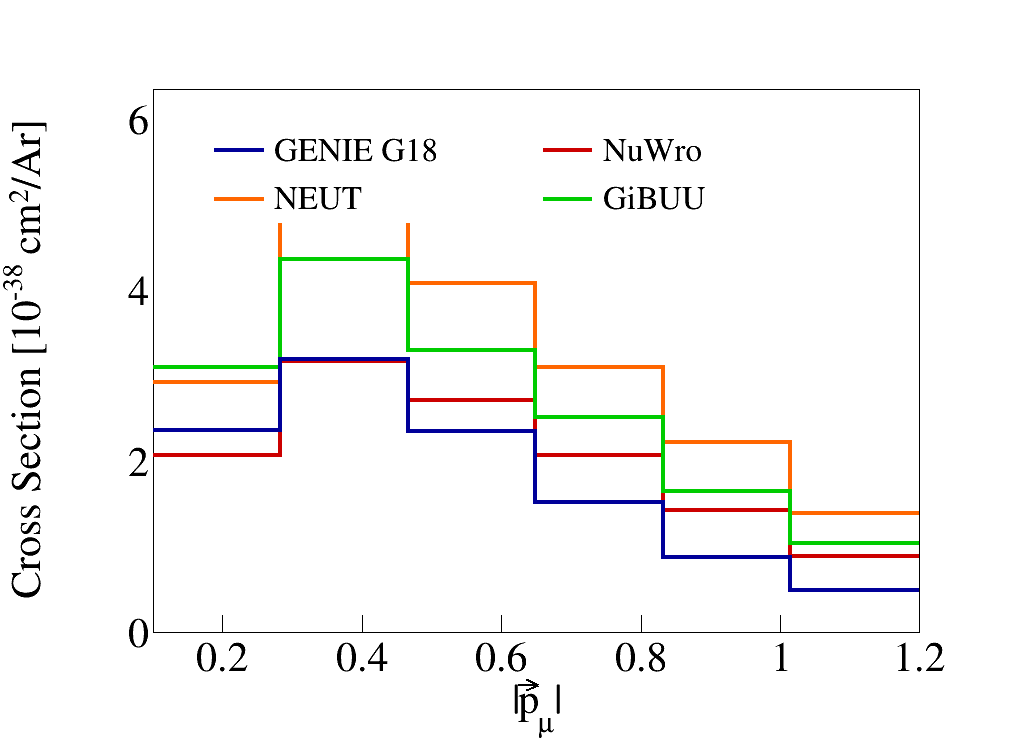
\includegraphics[width=3in]{../Figs/Overlay/PostFSI/Overlay_TrueMuonMomentumPlot.png}}
    \subfloat{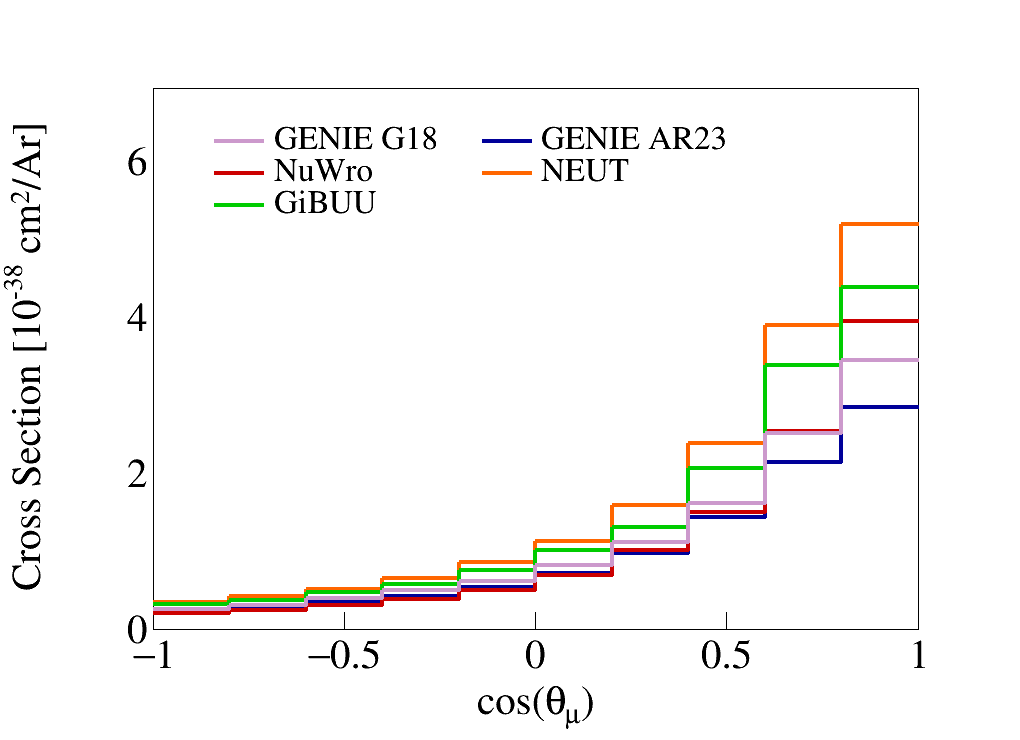
\includegraphics[width=3in]{../Figs/Overlay/PostFSI/Overlay_TrueMuonCosThetaPlot.png}} \\
    \subfloat{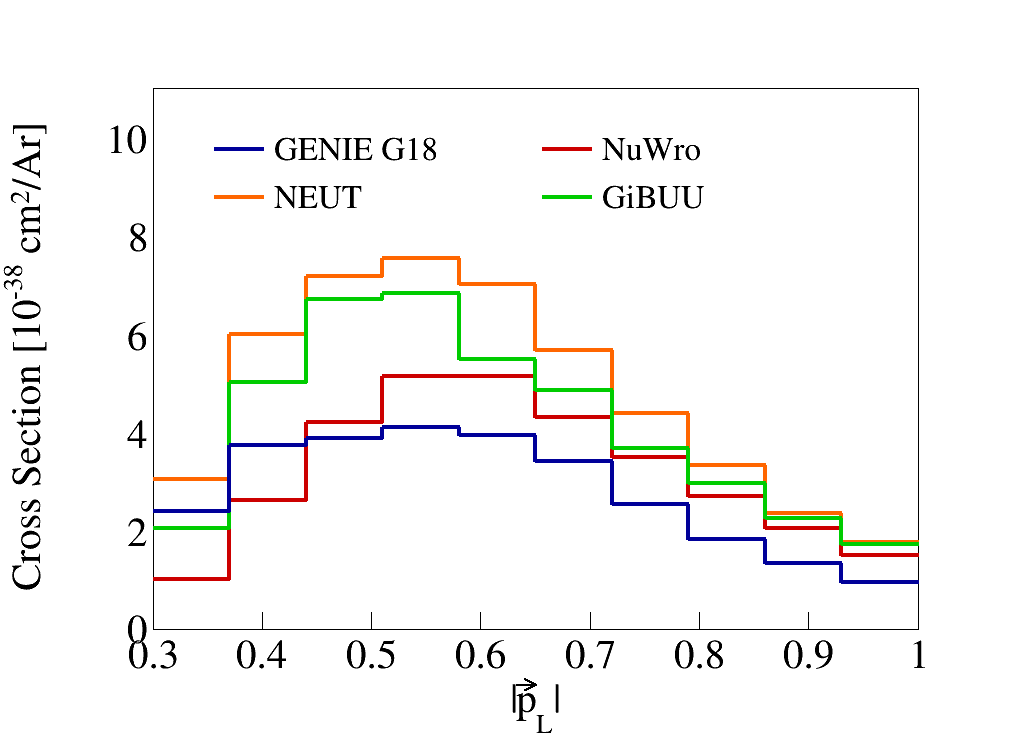
\includegraphics[width=3in]{../Figs/Overlay/PostFSI/Overlay_TrueLeadingProtonMomentumPlot.png}}
    \subfloat{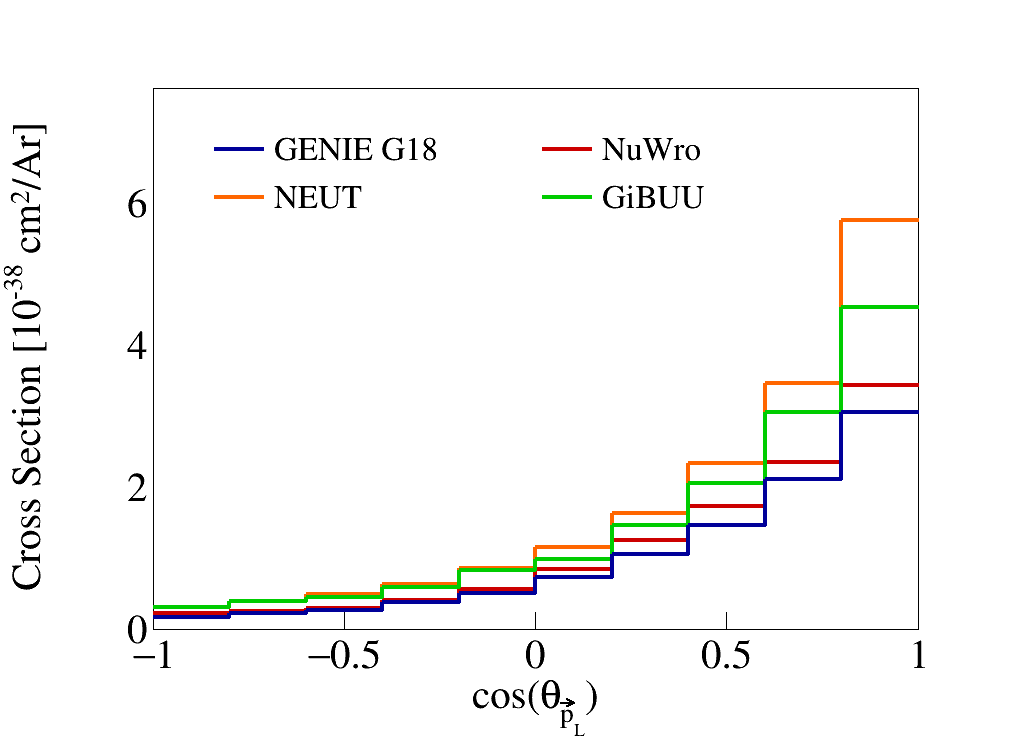
\includegraphics[width=3in]{../Figs/Overlay/PostFSI/Overlay_TrueLeadingProtonCosThetaPlot.png}} \\
    \subfloat{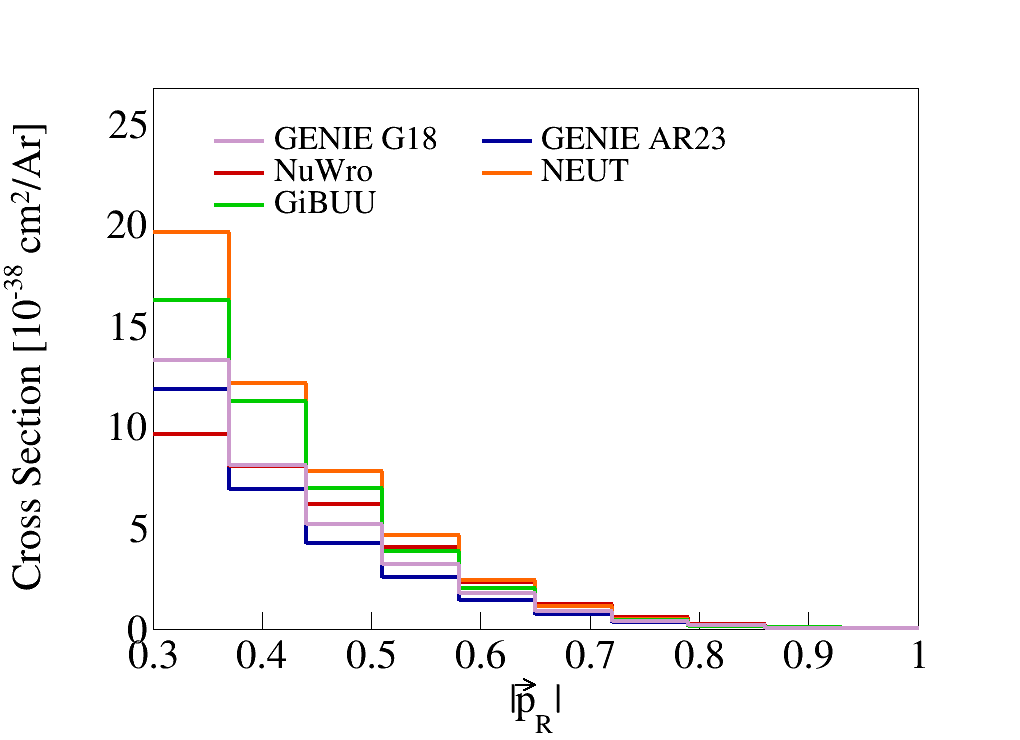
\includegraphics[width=3in]{../Figs/Overlay/PostFSI/Overlay_TrueRecoilProtonMomentumPlot.png}}
    \subfloat{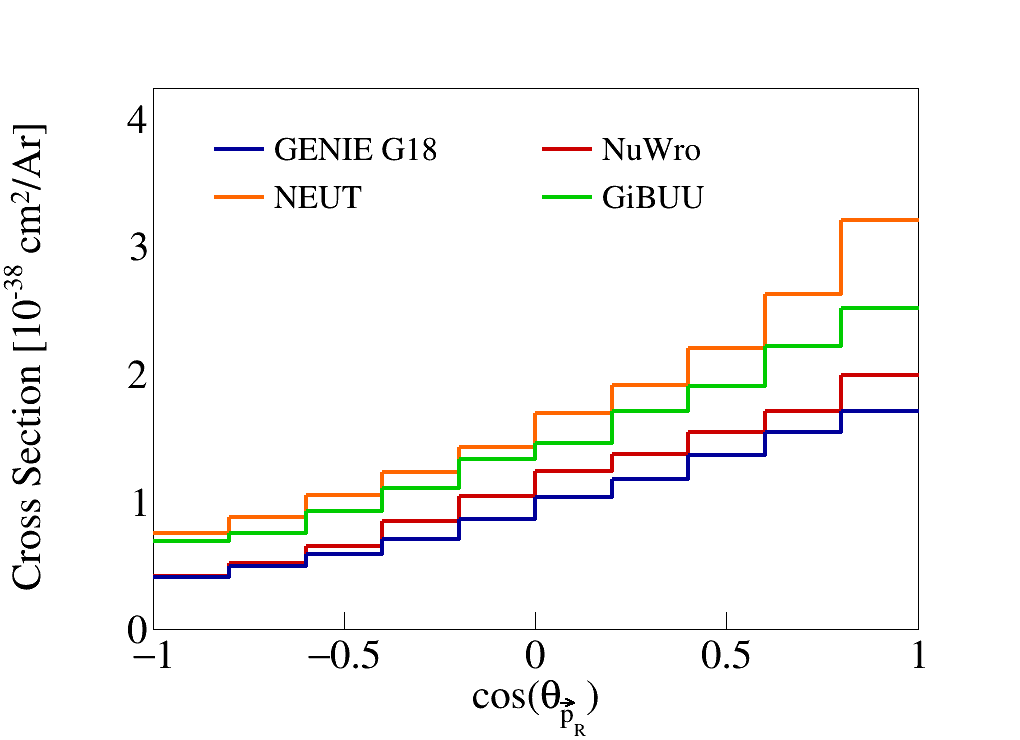
\includegraphics[width=3in]{../Figs/Overlay/PostFSI/Overlay_TrueRecoilProtonCosThetaPlot.png}} \\
    \caption{Cross sections for momentum and opening angles of individual particles.}
    \label{fig:momenta-cos-theta}
\end{figure}

\afterpage{\clearpage}

We also define variables relating the multiple momentum vectors. First, the opening angle between the protons in the lab frame, given by 
\begin{align}
    \cos\left(\theta_{\vlp,\vrp}\right) = \frac{\vlp \cdot \vrp}{|\vlp||\vrp|}.
\end{align}
Then, the opening angle between the total proton momentum ($\vtp = \vlp + \vrp$) and the muon, given by 
\begin{align}
    \cos\left(\theta_{\vm,\vtp}\right) = \frac{\vm \cdot \vtp}{|\vm||\vtp|}.
\end{align}
The momentum transverse to the direction of the neutrino beam, which we denote $\vdp$ and is given by 
\begin{align}
    \vdp = \vec{p}^{\mu}_T + \vec{p}^{L}_T + \vec{p}^{R}_T.
\end{align}
For the transverse momentum, we will be interested in its magnitude $|\vdp|$. 
Finally, the angular orientation of the transverse momentum with respect to the transverse muon 
is defined as 
\begin{align}
    \delta \alpha_T = \cos^{-1}\left(\frac{- \vec{p}^\mu_T \cdot \vdp}{|\vec{p}^\mu_T||\vdp|}\right).
\end{align}
We plot the differential cross sections of these variables for the given generators in Figure~\ref{fig:angles-transverse-momentum}.
We can also see the cross section by event type for all variables and all generators in 
Figures~\labelcref{fig:inte-breakdown-muon-momentum,fig:inte-breakdown-muon-cos-theta,fig:inte-breakdown-lp-momentum,fig:inte-breakdown-lp-cos-theta,fig:inte-breakdown-rp-momentum,fig:inte-breakdown-rp-cos-theta,fig:inte-breakdown-delta-alpha-t,fig:inte-breakdown-dpt,fig:inte-breakdown-cos-opening-angle-protons,fig:inte-breakdown-cos-opening-angle-muon-total-proton}.

\begin{figure}
    \centering
    \subfloat{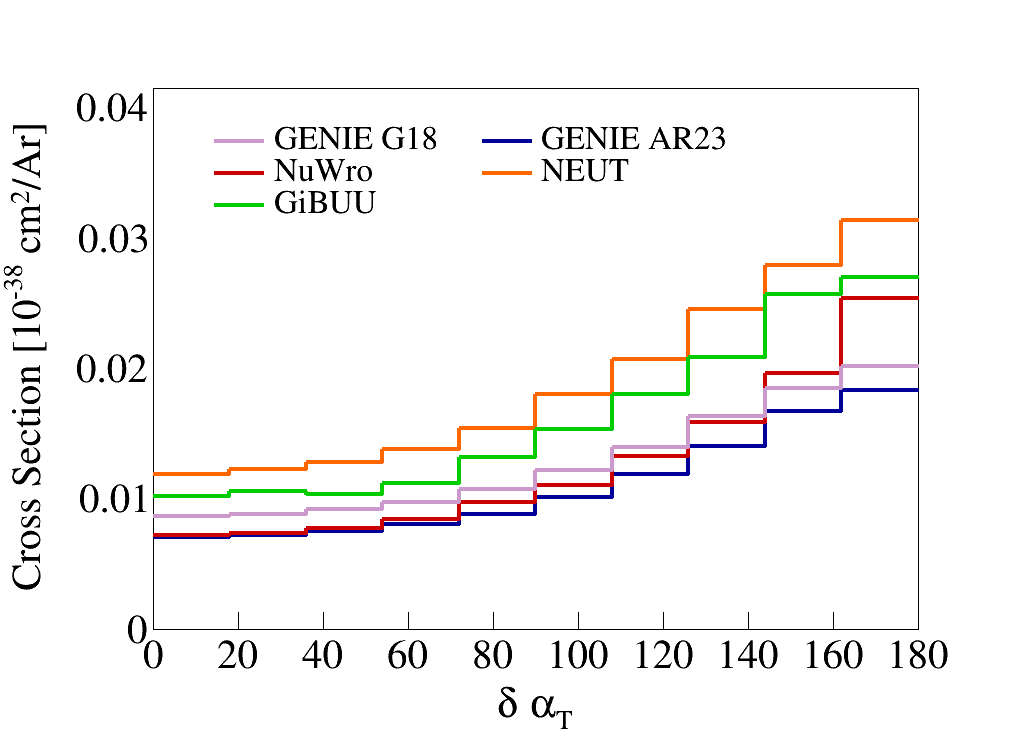
\includegraphics[width=3in]{../Figs/Overlay/PostFSI/Overlay_TrueDeltaAlphaTPlot.png}}
    \subfloat{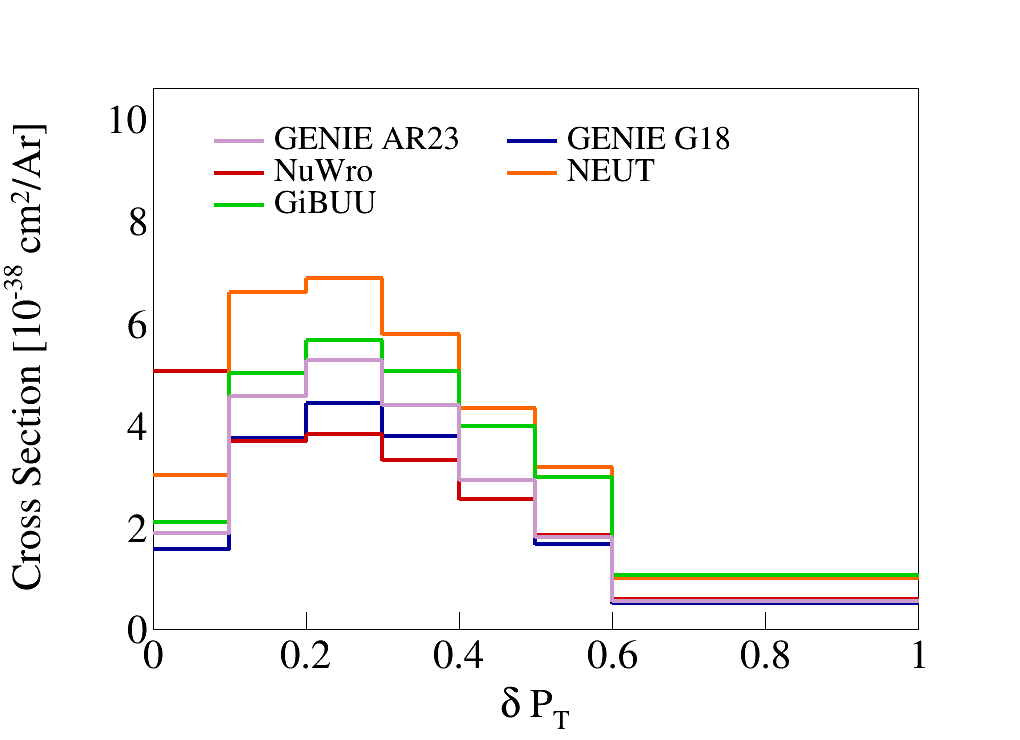
\includegraphics[width=3in]{../Figs/Overlay/PostFSI/Overlay_TrueTransverseMomentumPlot.png}} \\
    \subfloat{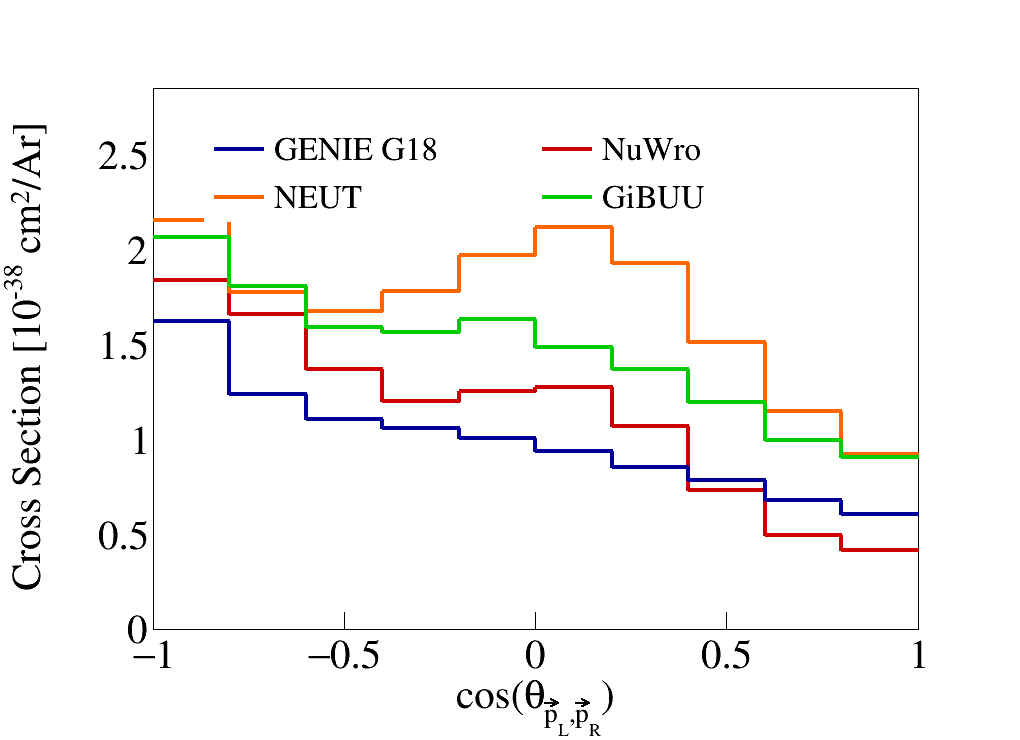
\includegraphics[width=3in]{../Figs/Overlay/PostFSI/Overlay_TrueCosOpeningAngleProtonsPlot.png}}
    \subfloat{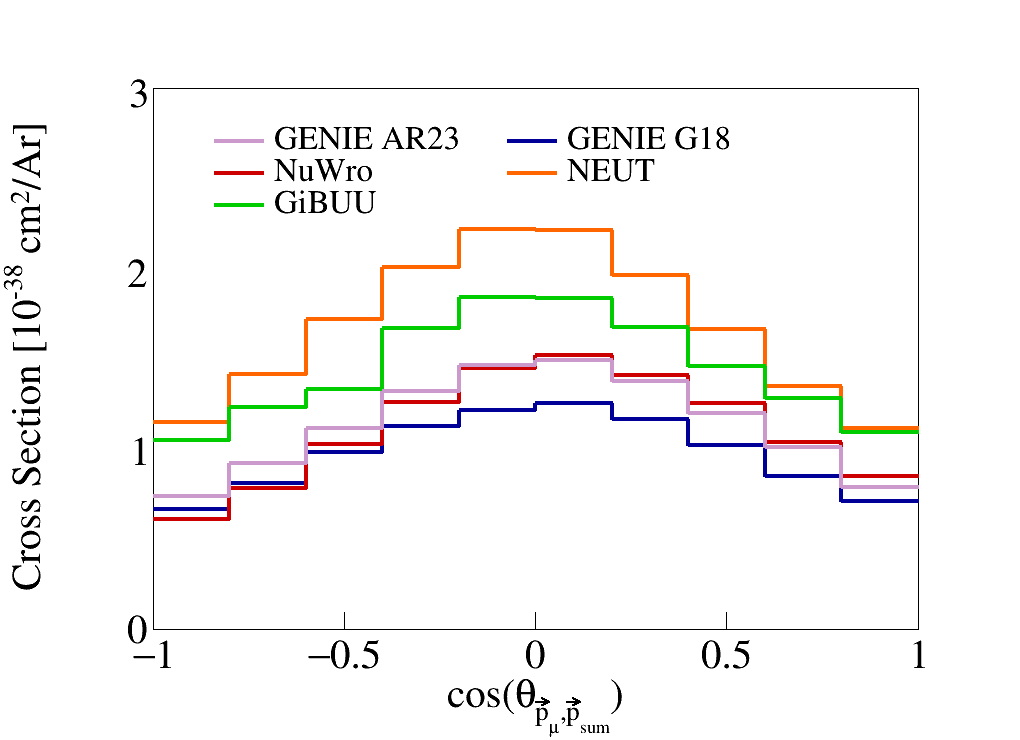
\includegraphics[width=3in]{../Figs/Overlay/PostFSI/Overlay_TrueCosOpeningAngleMuonTotalProtonPlot.png}} 
    \caption{Cross sections for opening angles and transverse momentum.}
    \label{fig:angles-transverse-momentum}
\end{figure}

\begin{figure}
    \centering
    \subfloat{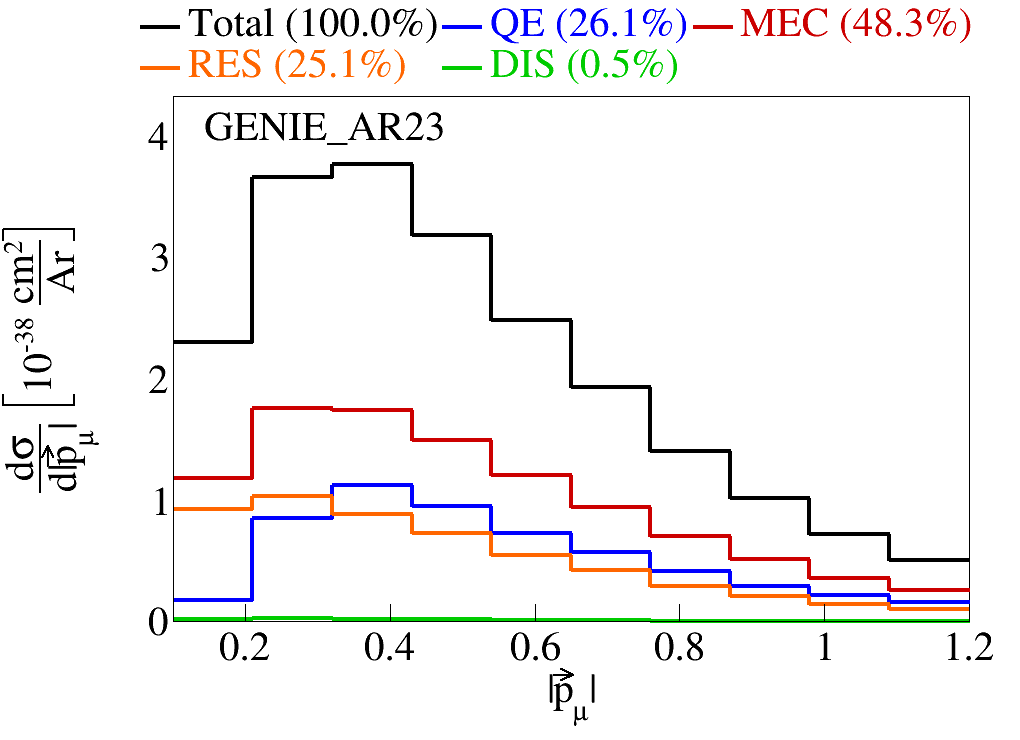
\includegraphics[width=3in]{../Figs/InteBreakDown/PostFSI/InteBreakDown_GENIE_AR23_TrueMuonMomentumPlot.png}}
    \subfloat{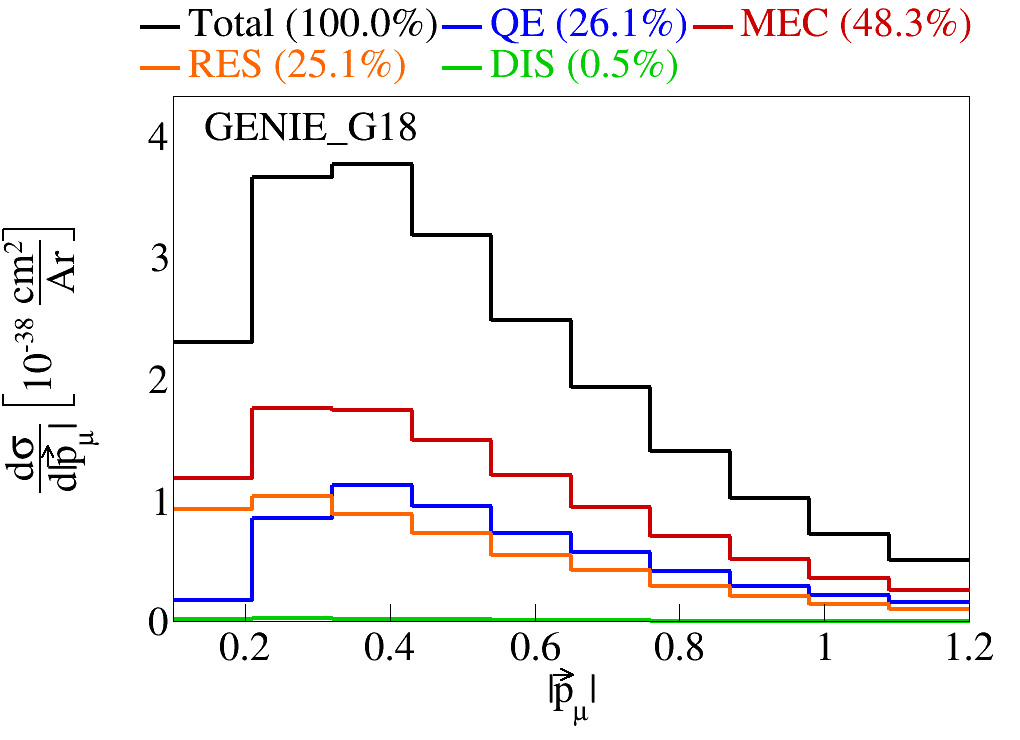
\includegraphics[width=3in]{../Figs/InteBreakDown/PostFSI/InteBreakDown_GENIE_G18_TrueMuonMomentumPlot.png}} \\
    \subfloat{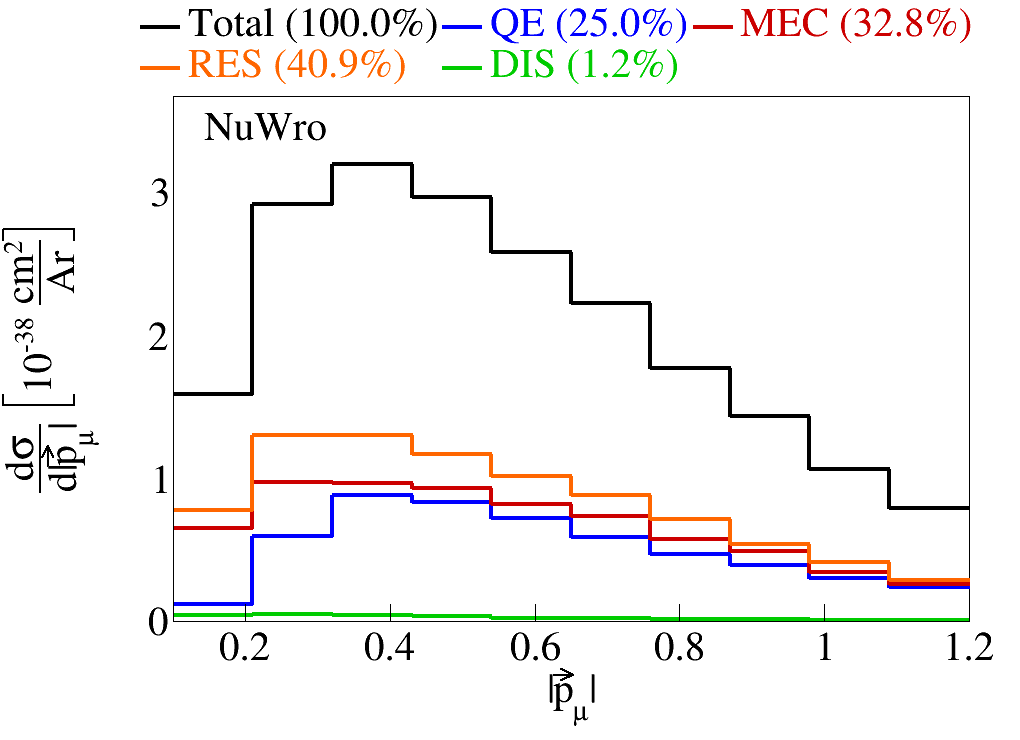
\includegraphics[width=3in]{../Figs/InteBreakDown/PostFSI/InteBreakDown_NuWro_TrueMuonMomentumPlot.png}}
    \subfloat{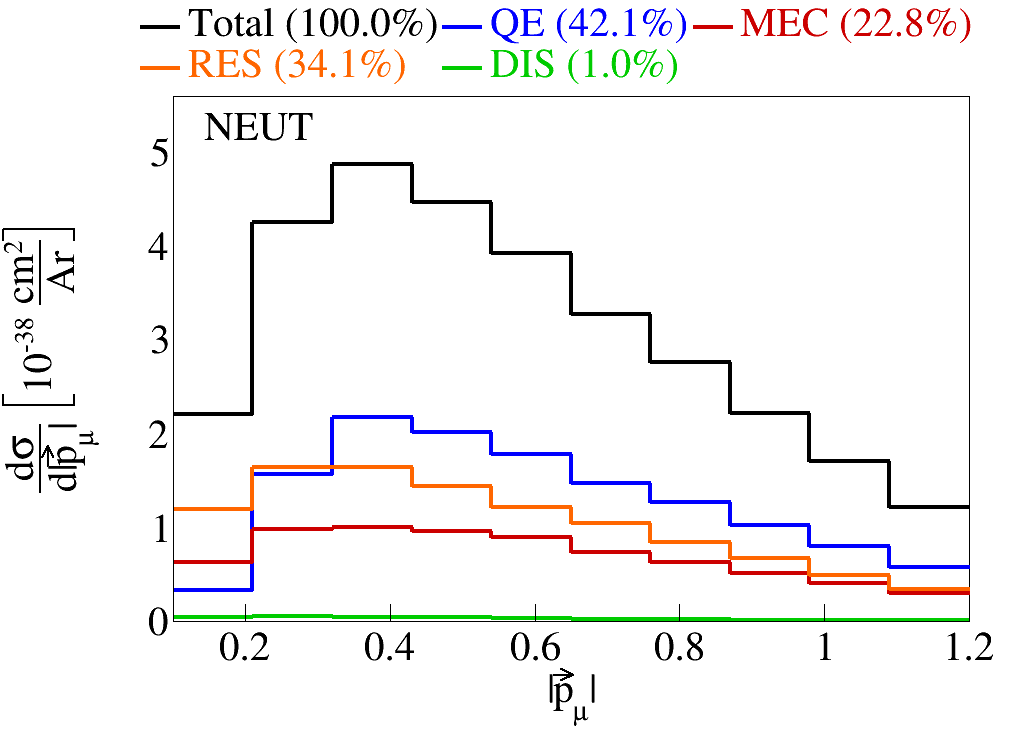
\includegraphics[width=3in]{../Figs/InteBreakDown/PostFSI/InteBreakDown_NEUT_TrueMuonMomentumPlot.png}} \\
    \subfloat{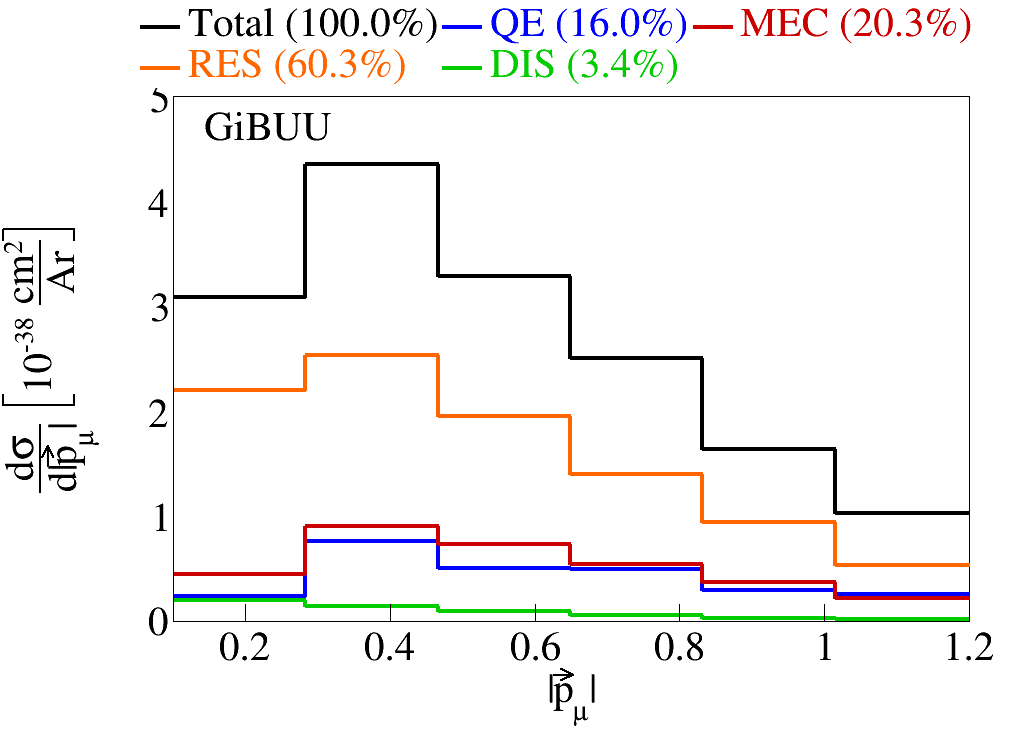
\includegraphics[width=3in]{../Figs/InteBreakDown/PostFSI/InteBreakDown_GiBUU_TrueMuonMomentumPlot.png}}
    \caption{Event interaction breakdown for $|\vm|$.}
    \label{fig:inte-breakdown-muon-momentum}
\end{figure}

\begin{figure}
    \centering
    \subfloat{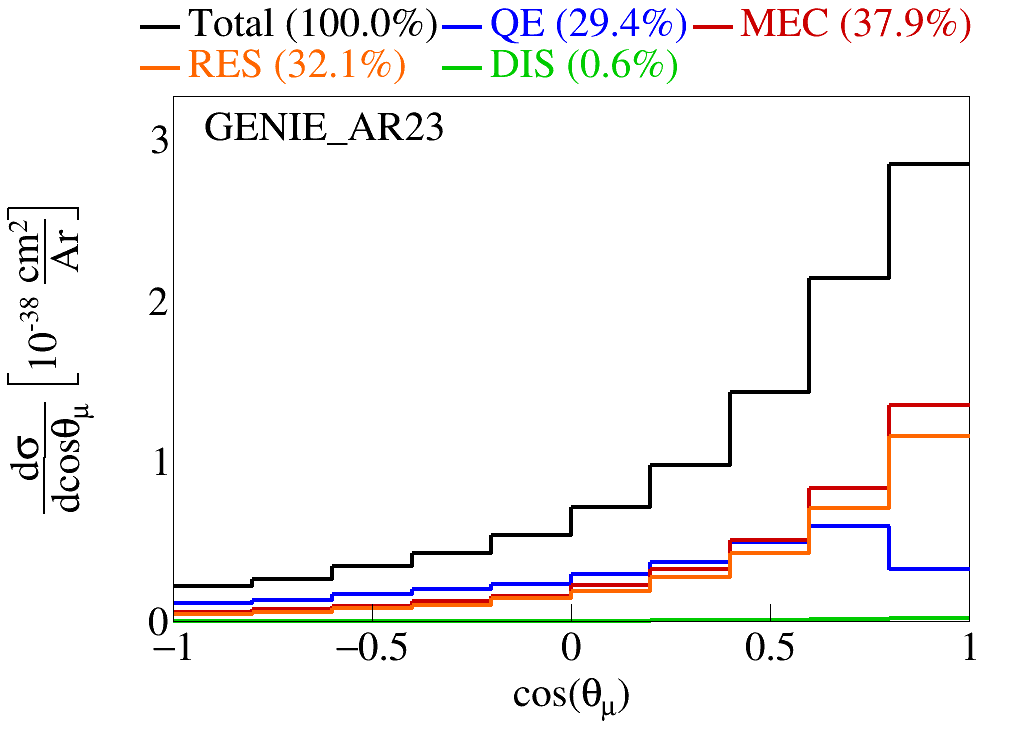
\includegraphics[width=3in]{../Figs/InteBreakDown/PostFSI/InteBreakDown_GENIE_AR23_TrueMuonCosThetaPlot.png}}
    \subfloat{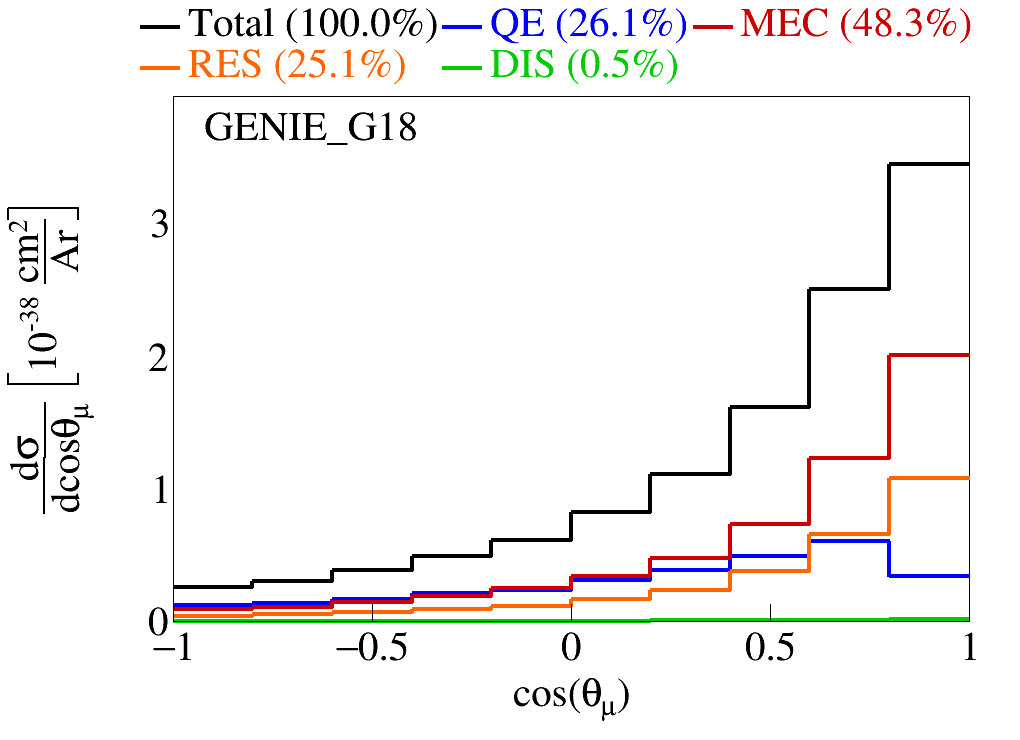
\includegraphics[width=3in]{../Figs/InteBreakDown/PostFSI/InteBreakDown_GENIE_G18_TrueMuonCosThetaPlot.png}} \\
    \subfloat{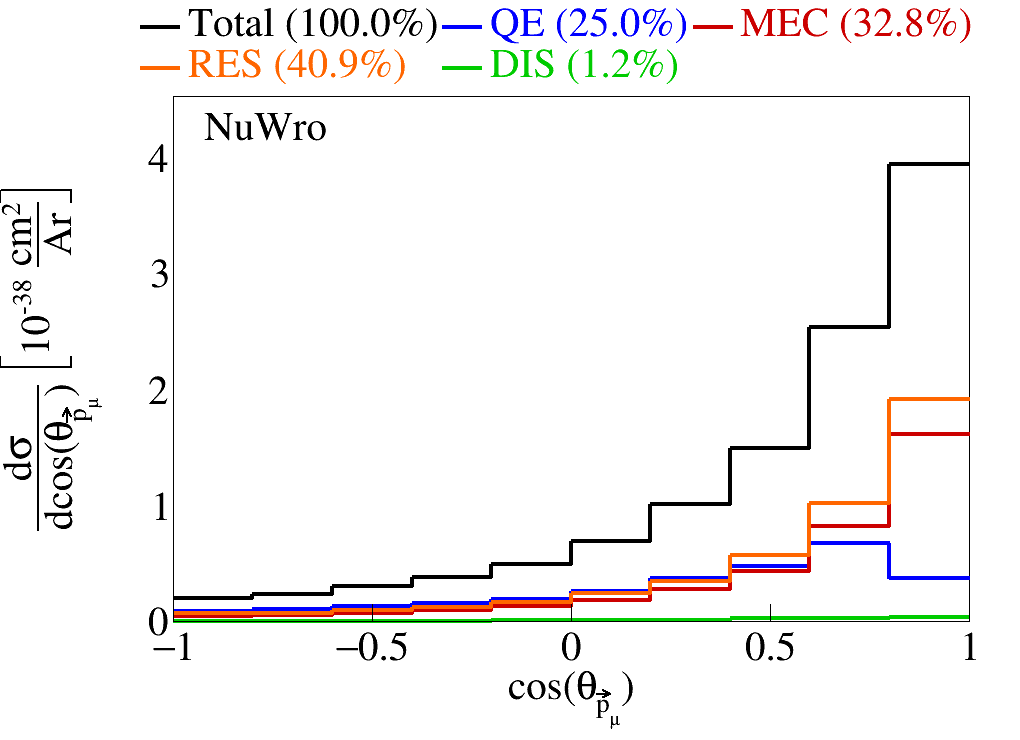
\includegraphics[width=3in]{../Figs/InteBreakDown/PostFSI/InteBreakDown_NuWro_TrueMuonCosThetaPlot.png}}
    \subfloat{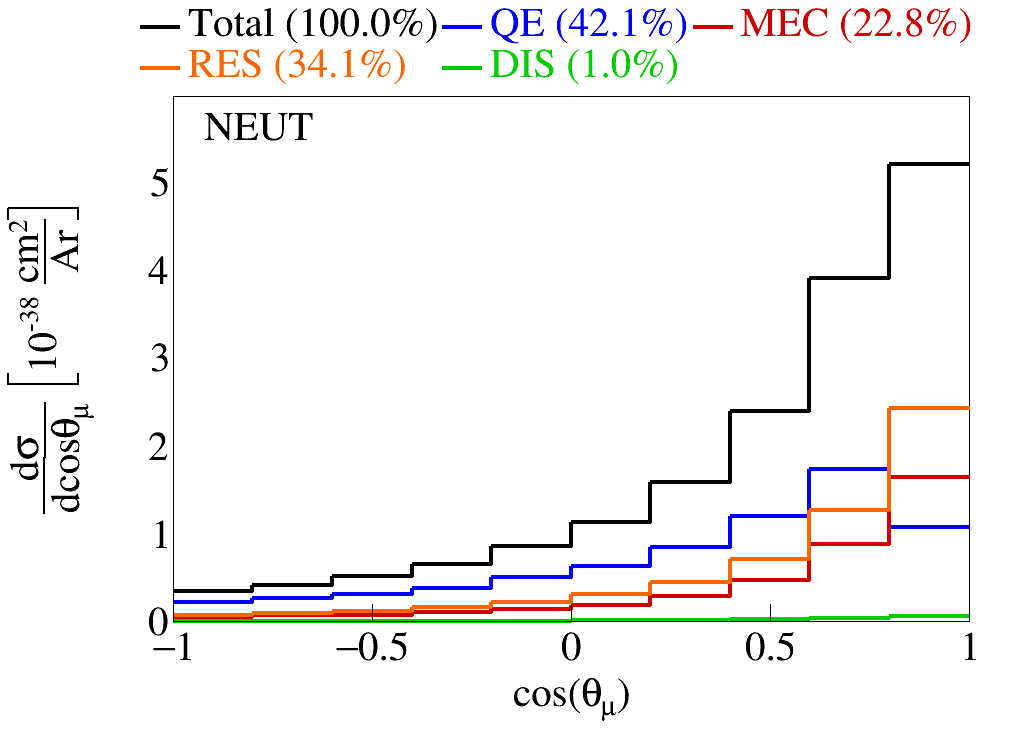
\includegraphics[width=3in]{../Figs/InteBreakDown/PostFSI/InteBreakDown_NEUT_TrueMuonCosThetaPlot.png}} \\
    \subfloat{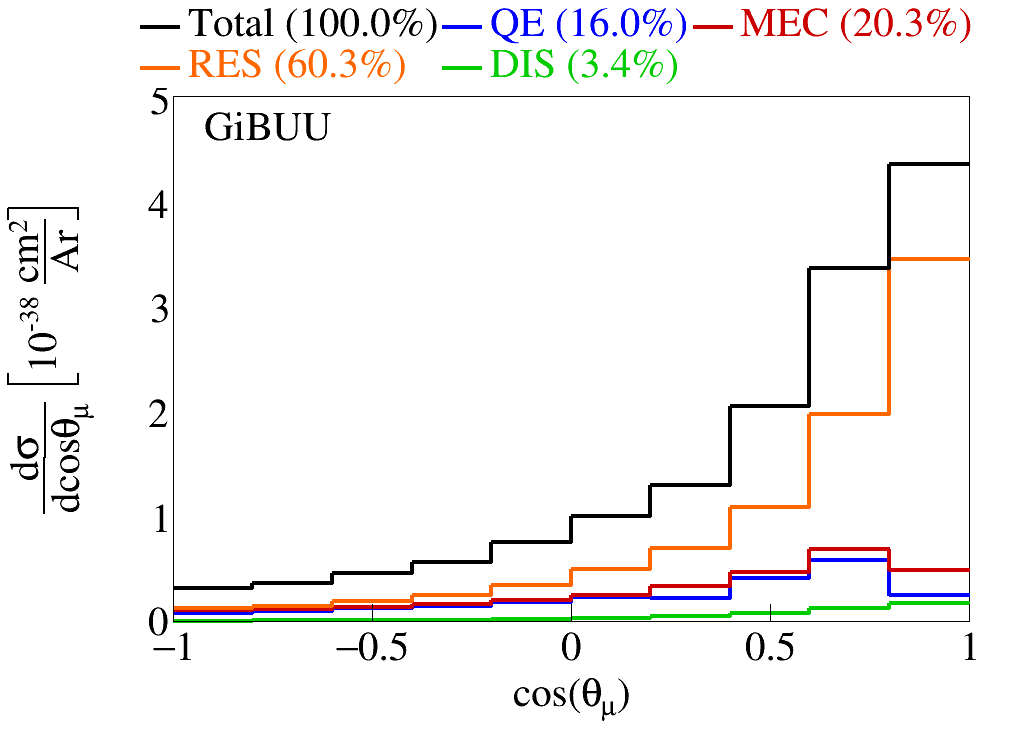
\includegraphics[width=3in]{../Figs/InteBreakDown/PostFSI/InteBreakDown_GiBUU_TrueMuonCosThetaPlot.png}}
    \caption{Event interaction breakdown for $\cos(\theta_{\vm})$.}
    \label{fig:inte-breakdown-muon-cos-theta}
\end{figure}

\begin{figure}
    \centering
    \subfloat{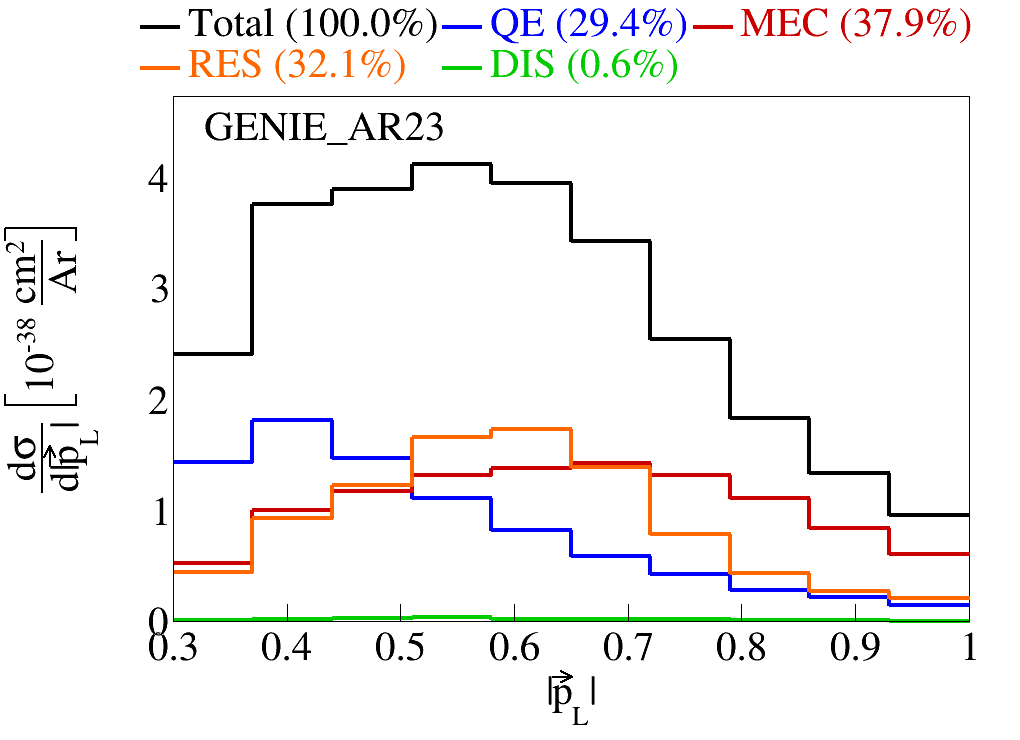
\includegraphics[width=3in]{../Figs/InteBreakDown/PostFSI/InteBreakDown_GENIE_AR23_TrueLeadingProtonMomentumPlot.png}}
    \subfloat{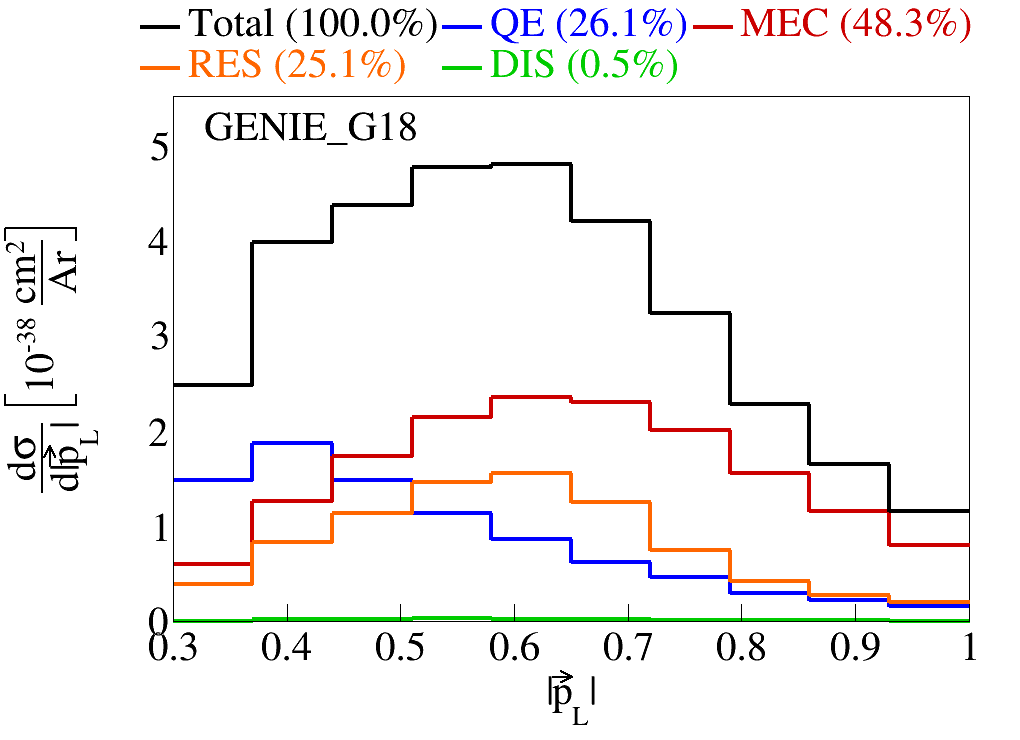
\includegraphics[width=3in]{../Figs/InteBreakDown/PostFSI/InteBreakDown_GENIE_G18_TrueLeadingProtonMomentumPlot.png}} \\
    \subfloat{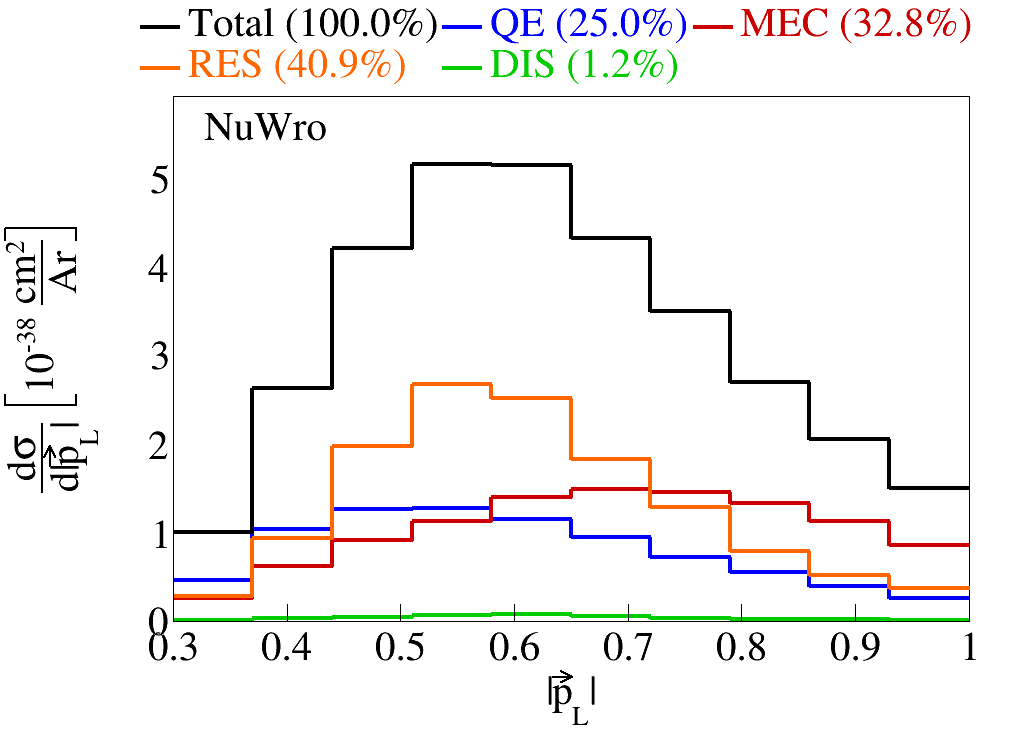
\includegraphics[width=3in]{../Figs/InteBreakDown/PostFSI/InteBreakDown_NuWro_TrueLeadingProtonMomentumPlot.png}}
    \subfloat{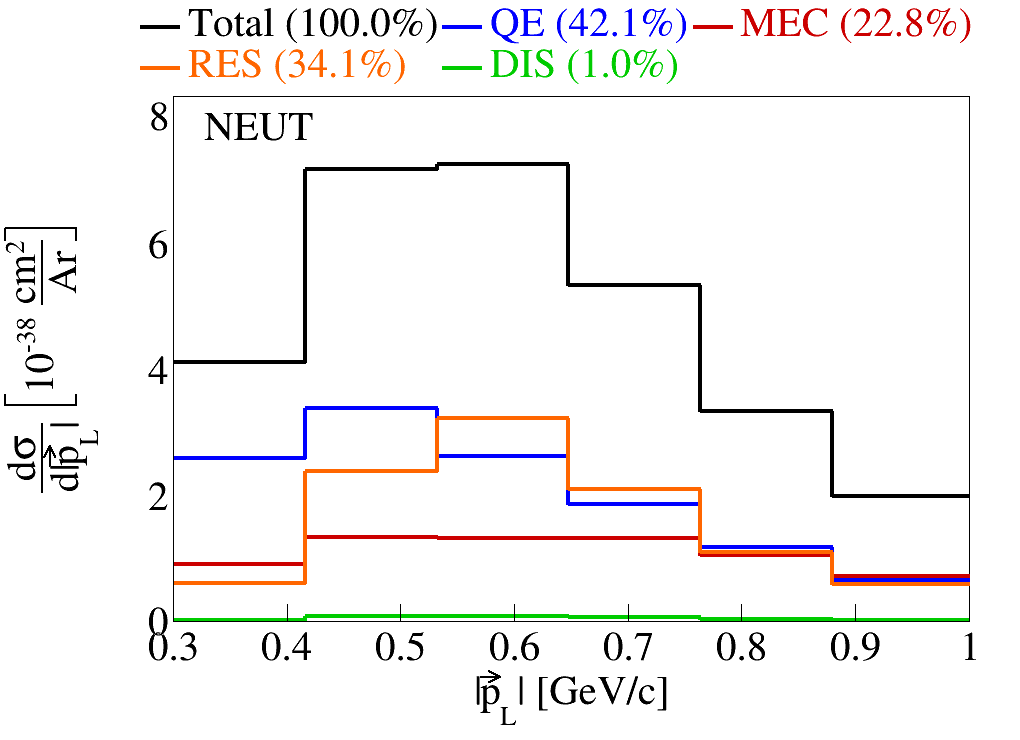
\includegraphics[width=3in]{../Figs/InteBreakDown/PostFSI/InteBreakDown_NEUT_TrueLeadingProtonMomentumPlot.png}} \\
    \subfloat{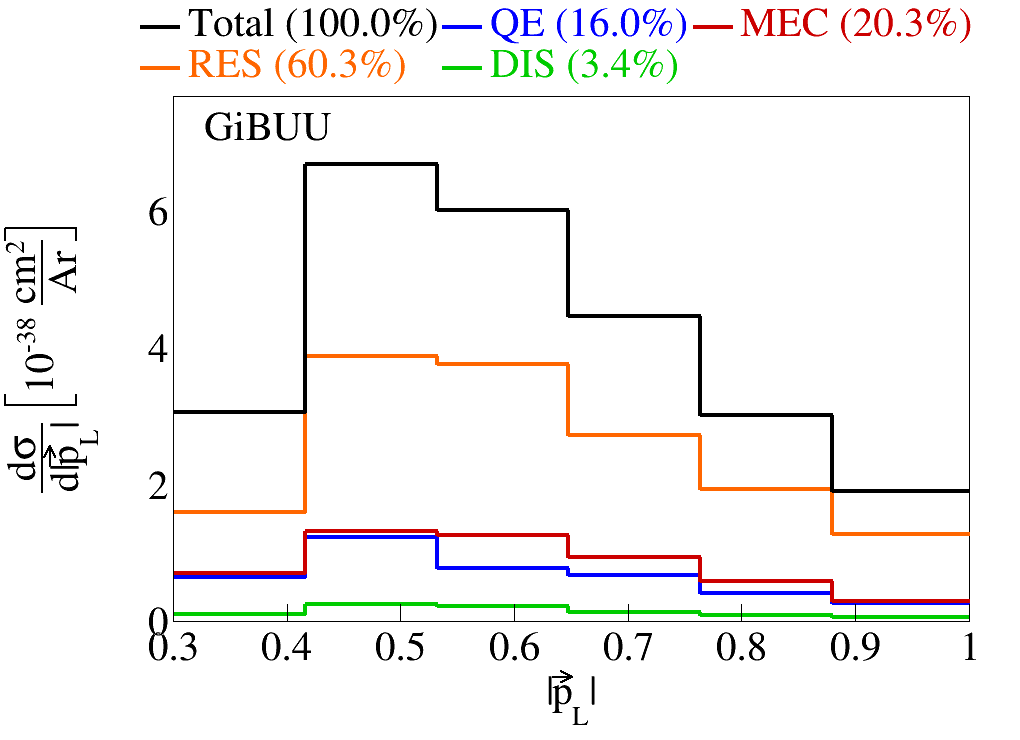
\includegraphics[width=3in]{../Figs/InteBreakDown/PostFSI/InteBreakDown_GiBUU_TrueLeadingProtonMomentumPlot.png}}
    \caption{Event interaction breakdown for $|\vlp|$.}
    \label{fig:inte-breakdown-lp-momentum}
\end{figure}

\begin{figure}
    \centering
    \subfloat{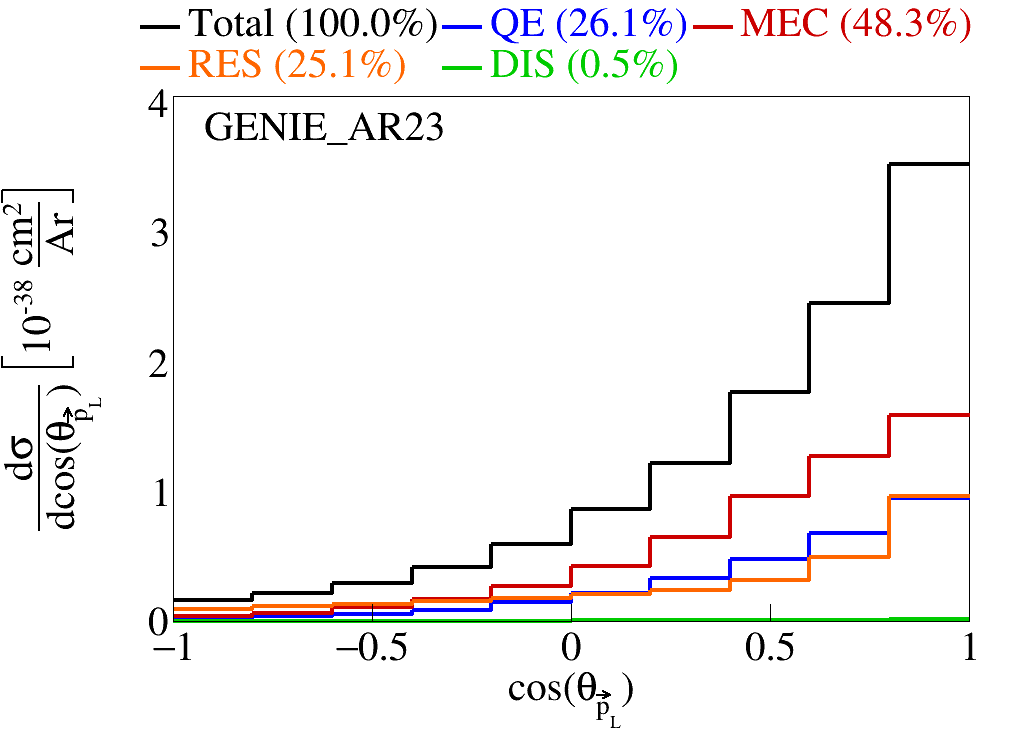
\includegraphics[width=3in]{../Figs/InteBreakDown/PostFSI/InteBreakDown_GENIE_AR23_TrueLeadingProtonCosThetaPlot.png}}
    \subfloat{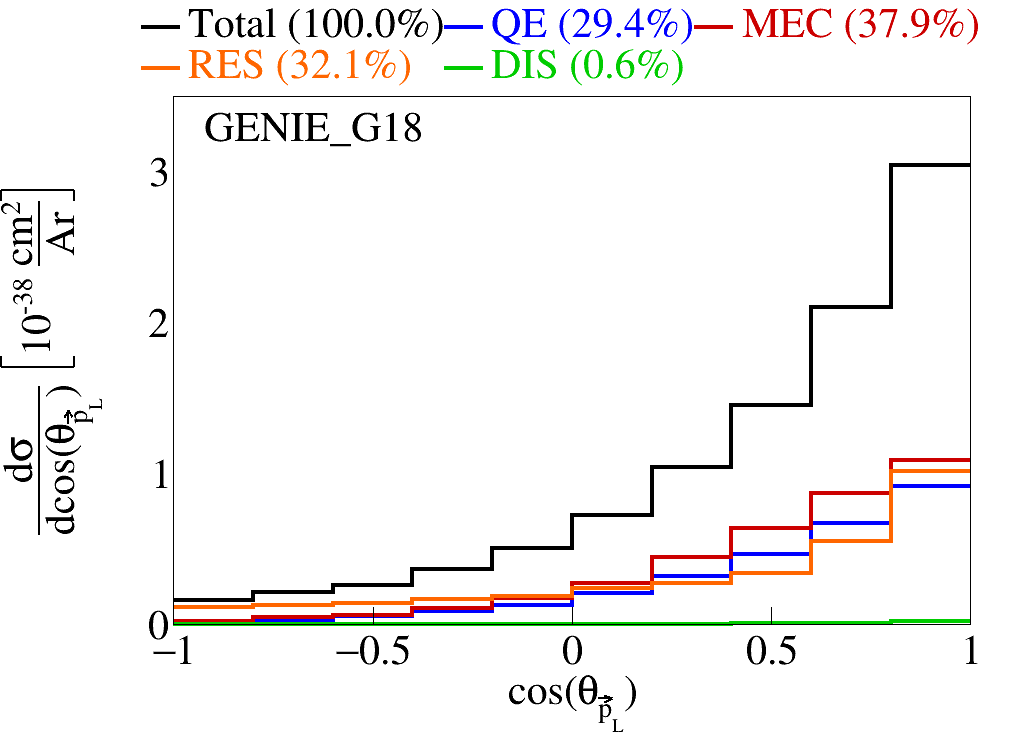
\includegraphics[width=3in]{../Figs/InteBreakDown/PostFSI/InteBreakDown_GENIE_G18_TrueLeadingProtonCosThetaPlot.png}} \\
    \subfloat{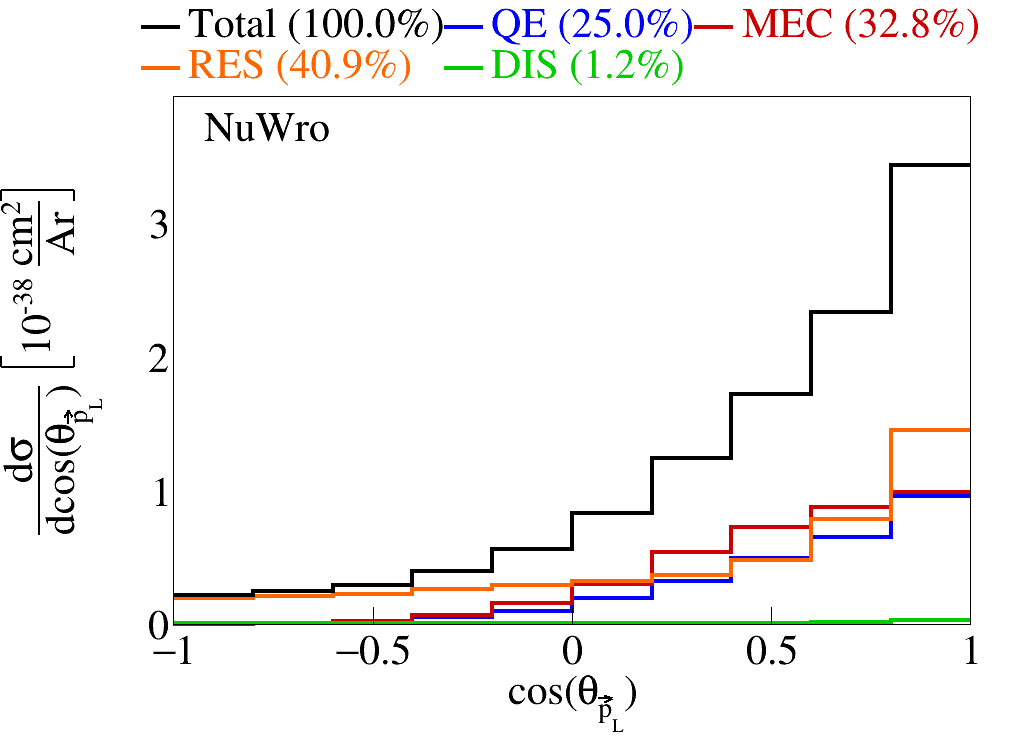
\includegraphics[width=3in]{../Figs/InteBreakDown/PostFSI/InteBreakDown_NuWro_TrueLeadingProtonCosThetaPlot.png}}
    \subfloat{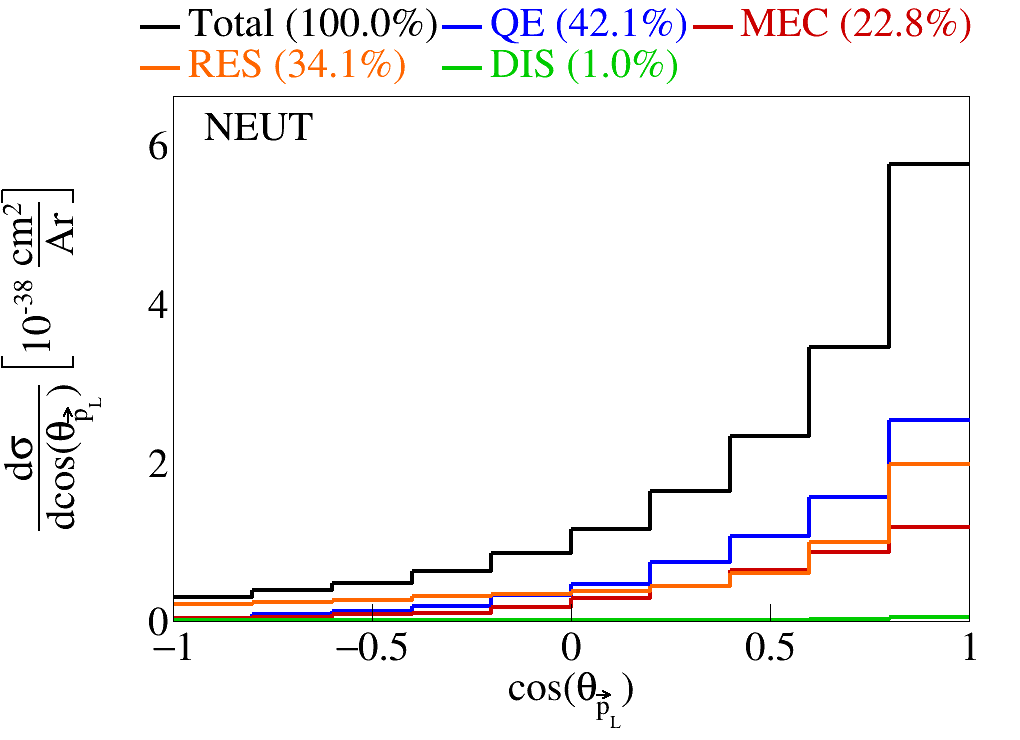
\includegraphics[width=3in]{../Figs/InteBreakDown/PostFSI/InteBreakDown_NEUT_TrueLeadingProtonCosThetaPlot.png}} \\
    \subfloat{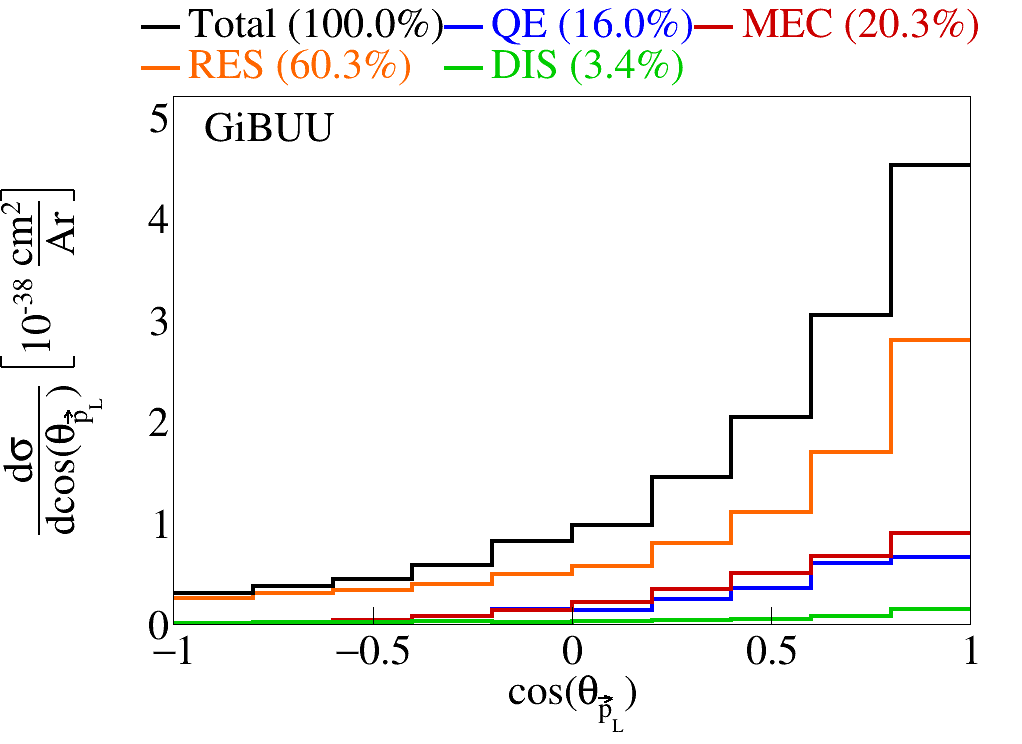
\includegraphics[width=3in]{../Figs/InteBreakDown/PostFSI/InteBreakDown_GiBUU_TrueLeadingProtonCosThetaPlot.png}}
    \caption{Event interaction breakdown for $\cos(\theta_{\vlp})$.}
    \label{fig:inte-breakdown-lp-cos-theta}
\end{figure}

\begin{figure}
    \centering
    \subfloat{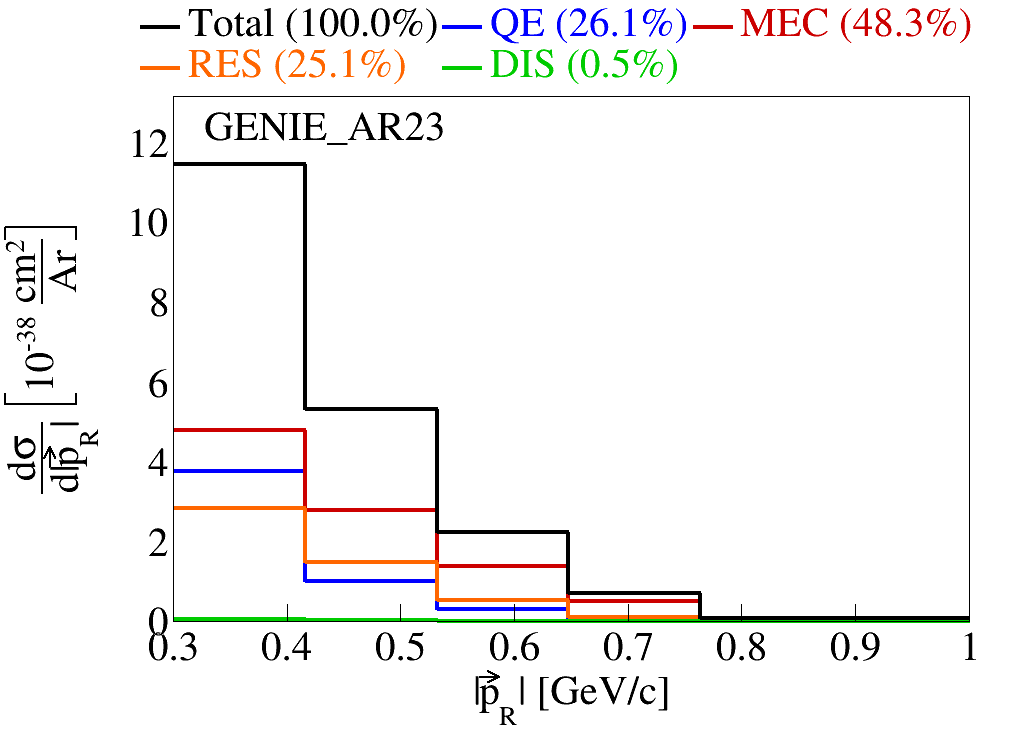
\includegraphics[width=3in]{../Figs/InteBreakDown/PostFSI/InteBreakDown_GENIE_AR23_TrueRecoilProtonMomentumPlot.png}}
    \subfloat{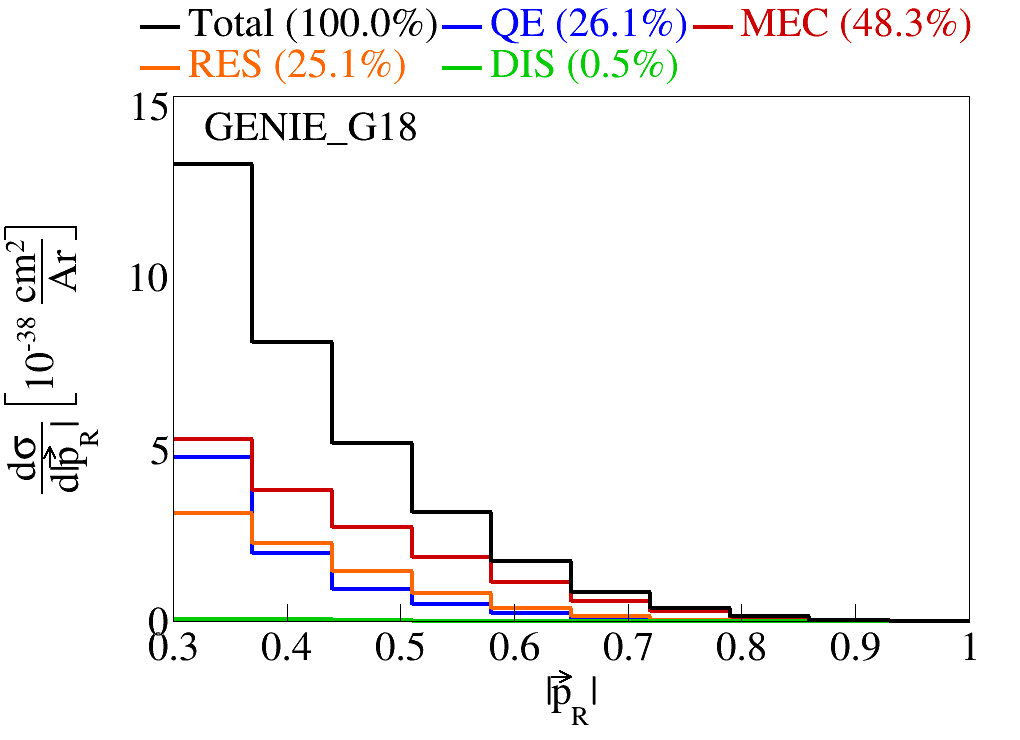
\includegraphics[width=3in]{../Figs/InteBreakDown/PostFSI/InteBreakDown_GENIE_G18_TrueRecoilProtonMomentumPlot.png}} \\
    \subfloat{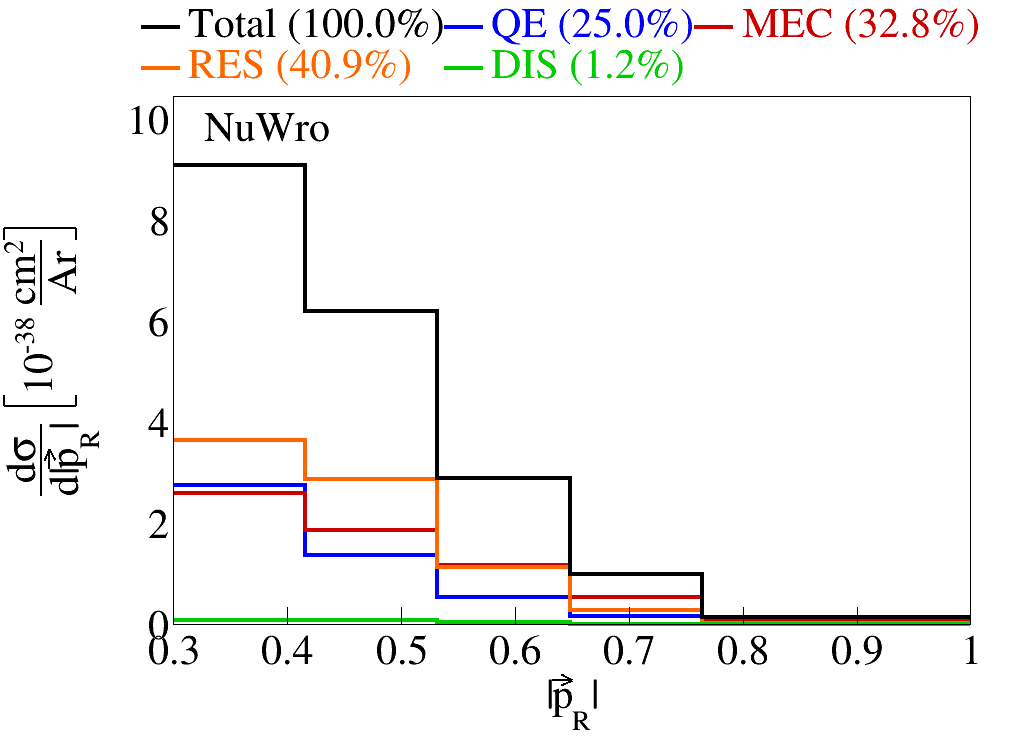
\includegraphics[width=3in]{../Figs/InteBreakDown/PostFSI/InteBreakDown_NuWro_TrueRecoilProtonMomentumPlot.png}}
    \subfloat{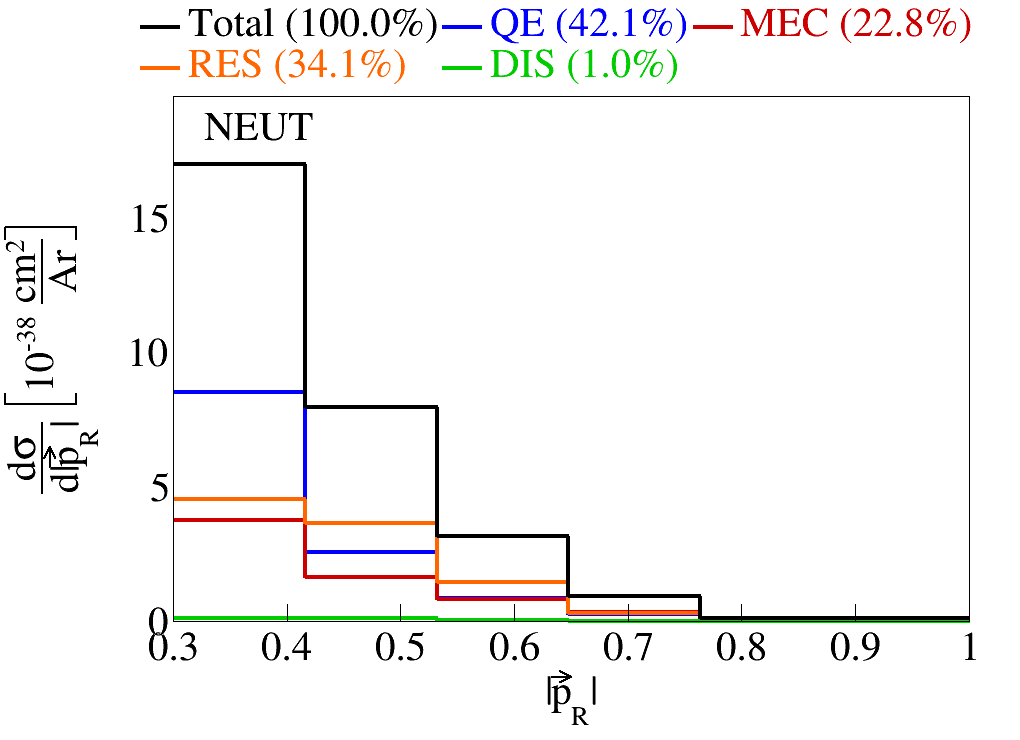
\includegraphics[width=3in]{../Figs/InteBreakDown/PostFSI/InteBreakDown_NEUT_TrueRecoilProtonMomentumPlot.png}} \\
    \subfloat{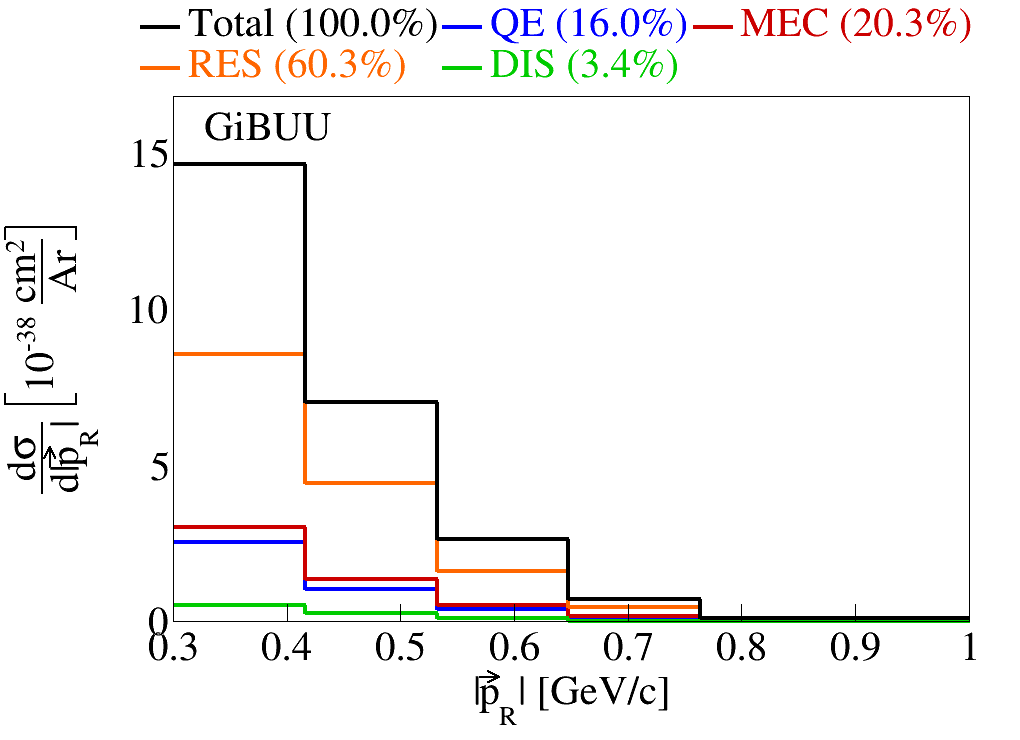
\includegraphics[width=3in]{../Figs/InteBreakDown/PostFSI/InteBreakDown_GiBUU_TrueRecoilProtonMomentumPlot.png}}
    \caption{Event interaction breakdown for $|\vrp|$.}
    \label{fig:inte-breakdown-rp-momentum}
\end{figure}

\begin{figure}
    \centering
    \subfloat{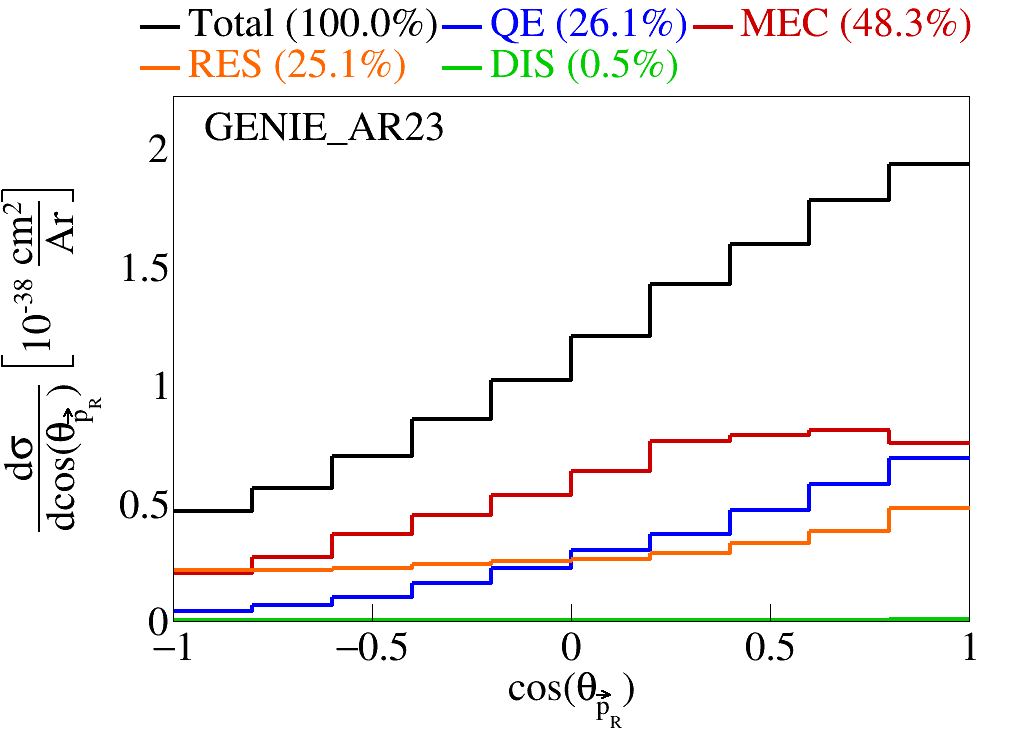
\includegraphics[width=3in]{../Figs/InteBreakDown/PostFSI/InteBreakDown_GENIE_AR23_TrueRecoilProtonCosThetaPlot.png}}
    \subfloat{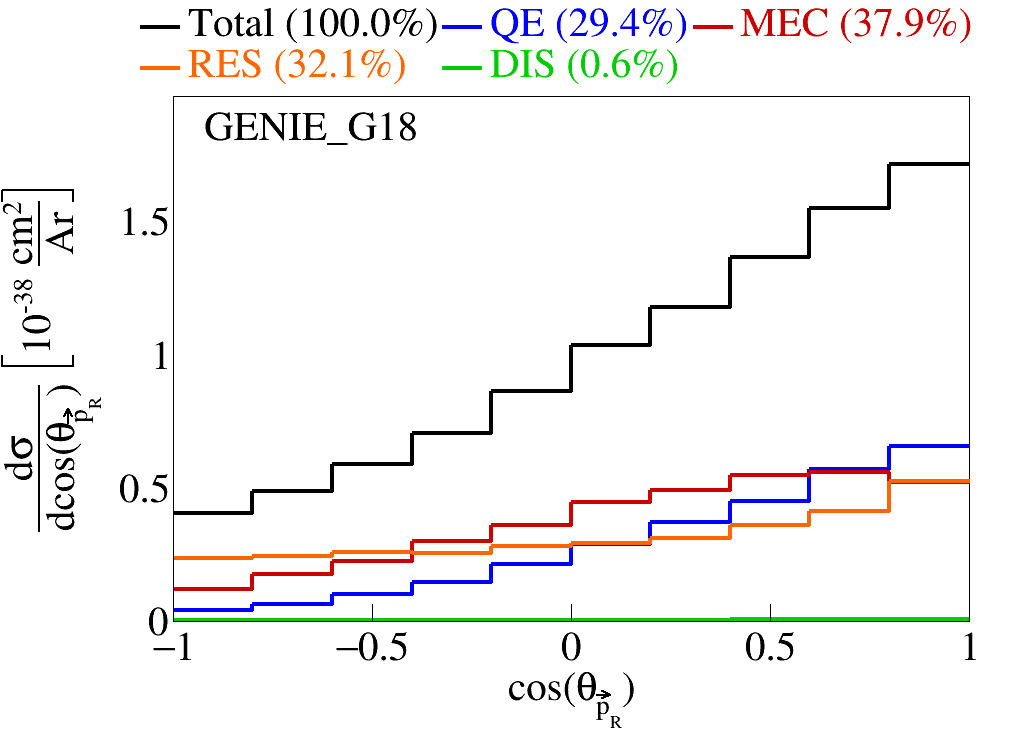
\includegraphics[width=3in]{../Figs/InteBreakDown/PostFSI/InteBreakDown_GENIE_G18_TrueRecoilProtonCosThetaPlot.png}} \\
    \subfloat{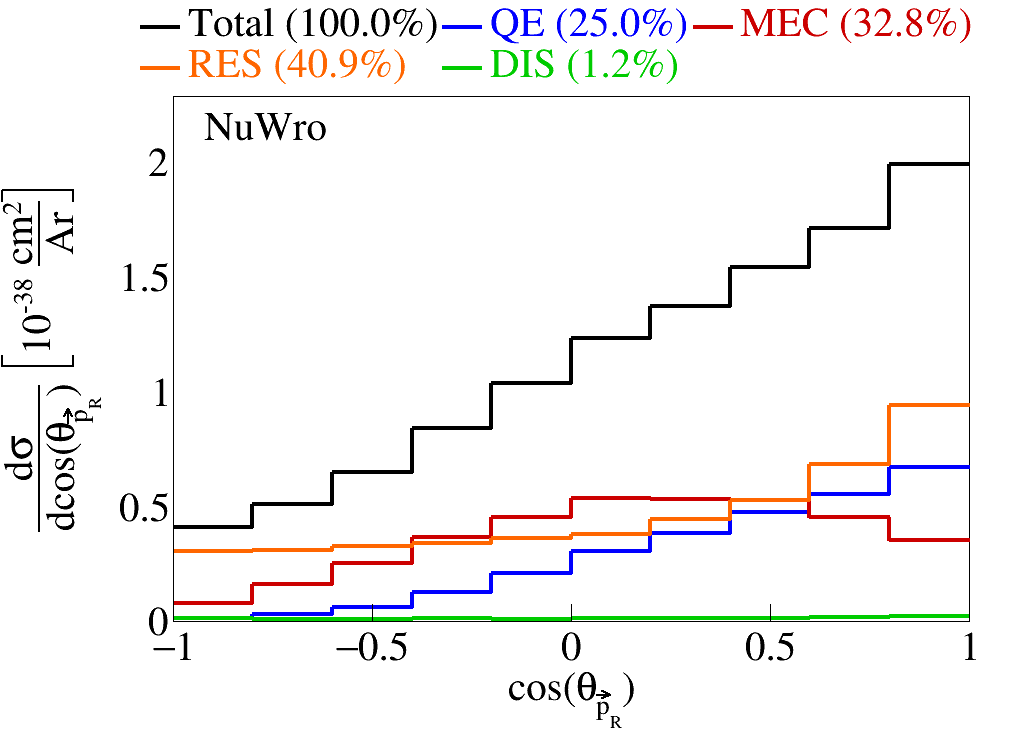
\includegraphics[width=3in]{../Figs/InteBreakDown/PostFSI/InteBreakDown_NuWro_TrueRecoilProtonCosThetaPlot.png}}
    \subfloat{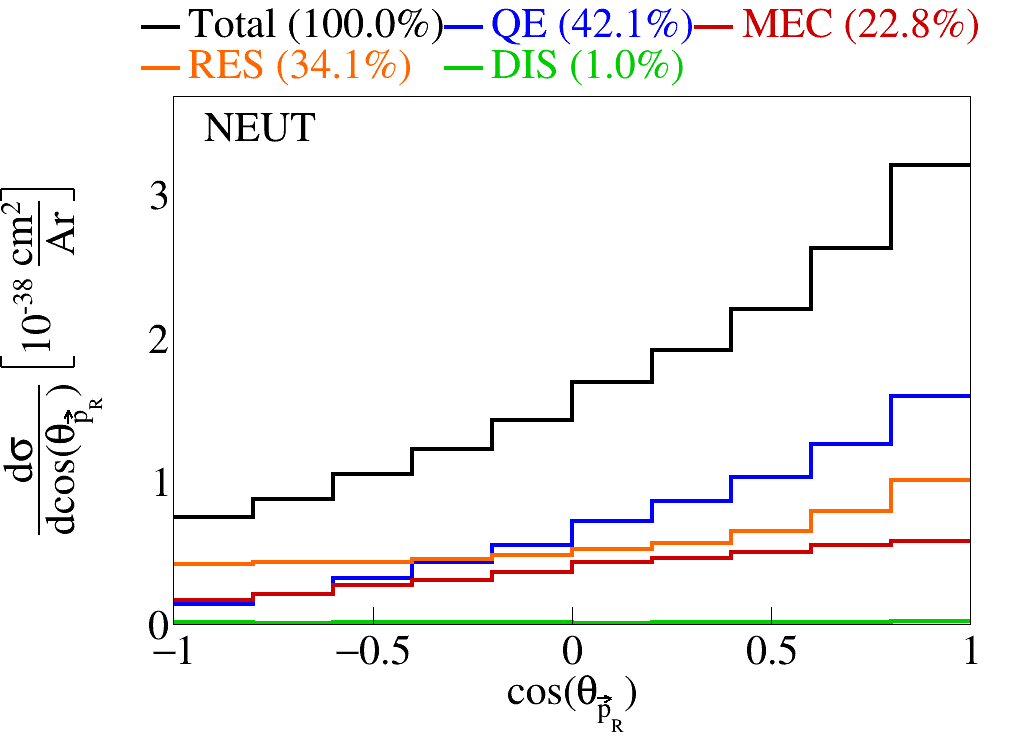
\includegraphics[width=3in]{../Figs/InteBreakDown/PostFSI/InteBreakDown_NEUT_TrueRecoilProtonCosThetaPlot.png}} \\
    \subfloat{\includegraphics[width=3in]{../Figs/InteBreakDown/PostFSI/InteBreakDown_GiBUU_TrueRecoilProtonCosThetaPlot.png}}
    \caption{Event interaction breakdown for $\cos(\theta_{\vrp})$.}
    \label{fig:inte-breakdown-rp-cos-theta}
\end{figure}

\begin{figure}
    \centering
    \subfloat{\includegraphics[width=3in]{../Figs/InteBreakDown/PostFSI/InteBreakDown_GENIE_AR23_TrueDeltaAlphaTPlot.png}}
    \subfloat{\includegraphics[width=3in]{../Figs/InteBreakDown/PostFSI/InteBreakDown_GENIE_G18_TrueDeltaAlphaTPlot.png}} \\
    \subfloat{\includegraphics[width=3in]{../Figs/InteBreakDown/PostFSI/InteBreakDown_NuWro_TrueDeltaAlphaTPlot.png}}
    \subfloat{\includegraphics[width=3in]{../Figs/InteBreakDown/PostFSI/InteBreakDown_NEUT_TrueDeltaAlphaTPlot.png}} \\
    \subfloat{\includegraphics[width=3in]{../Figs/InteBreakDown/PostFSI/InteBreakDown_GiBUU_TrueDeltaAlphaTPlot.png}}
    \caption{Event interaction breakdown for $\delta \alpha_T$.}
    \label{fig:inte-breakdown-delta-alpha-t}
\end{figure}

\begin{figure}
    \centering
    \subfloat{\includegraphics[width=3in]{../Figs/InteBreakDown/PostFSI/InteBreakDown_GENIE_AR23_TrueTransverseMomentumPlot.png}}
    \subfloat{\includegraphics[width=3in]{../Figs/InteBreakDown/PostFSI/InteBreakDown_GENIE_G18_TrueTransverseMomentumPlot.png}} \\
    \subfloat{\includegraphics[width=3in]{../Figs/InteBreakDown/PostFSI/InteBreakDown_NuWro_TrueTransverseMomentumPlot.png}}
    \subfloat{\includegraphics[width=3in]{../Figs/InteBreakDown/PostFSI/InteBreakDown_NEUT_TrueTransverseMomentumPlot.png}} \\
    \subfloat{\includegraphics[width=3in]{../Figs/InteBreakDown/PostFSI/InteBreakDown_GiBUU_TrueTransverseMomentumPlot.png}}
    \caption{Event interaction breakdown for $|\vdp|$.}
    \label{fig:inte-breakdown-dpt}
\end{figure}
\begin{figure}
    \centering
    \subfloat{\includegraphics[width=3in]{../Figs/InteBreakDown/PostFSI/InteBreakDown_GENIE_AR23_TrueCosOpeningAngleProtonsPlot.png}}
    \subfloat{\includegraphics[width=3in]{../Figs/InteBreakDown/PostFSI/InteBreakDown_GENIE_G18_TrueCosOpeningAngleProtonsPlot.png}} \\
    \subfloat{\includegraphics[width=3in]{../Figs/InteBreakDown/PostFSI/InteBreakDown_NuWro_TrueCosOpeningAngleProtonsPlot.png}}
    \subfloat{\includegraphics[width=3in]{../Figs/InteBreakDown/PostFSI/InteBreakDown_NEUT_TrueCosOpeningAngleProtonsPlot.png}} \\
    \subfloat{\includegraphics[width=3in]{../Figs/InteBreakDown/PostFSI/InteBreakDown_GiBUU_TrueCosOpeningAngleProtonsPlot.png}}
    \caption{Event interaction breakdown for $\cos(\theta_{\vlp,\vrp})$.}
    \label{fig:inte-breakdown-cos-opening-angle-protons}
\end{figure}

\begin{figure}
    \centering
    \subfloat{\includegraphics[width=3in]{../Figs/InteBreakDown/PostFSI/InteBreakDown_GENIE_AR23_TrueCosOpeningAngleMuonTotalProtonPlot.png}}
    \subfloat{\includegraphics[width=3in]{../Figs/InteBreakDown/PostFSI/InteBreakDown_GENIE_G18_TrueCosOpeningAngleMuonTotalProtonPlot.png}} \\
    \subfloat{\includegraphics[width=3in]{../Figs/InteBreakDown/PostFSI/InteBreakDown_NuWro_TrueCosOpeningAngleMuonTotalProtonPlot.png}}
    \subfloat{\includegraphics[width=3in]{../Figs/InteBreakDown/PostFSI/InteBreakDown_NEUT_TrueCosOpeningAngleMuonTotalProtonPlot.png}} \\
    \subfloat{\includegraphics[width=3in]{../Figs/InteBreakDown/PostFSI/InteBreakDown_GiBUU_TrueCosOpeningAngleMuonTotalProtonPlot.png}}
    \caption{Event interaction breakdown for $\cos(\theta_{\vm,\vtp})$.}
    \label{fig:inte-breakdown-cos-opening-angle-muon-total-proton}
\end{figure}

\clearpage

\subsection{Pre-FSI events}

To investigate why the percentage of MEC events for some generators is low, we performed event selection before any final state interactions took place and plotted the interaction breakdown. 
For both GENIE tunes, NEUT, and NuWro, we got 100\% MEC events pre-FSI. For GiBUU, only 4.1\% MEC versus 76.2\% RES and 16\% DIS events pre-FSI. 
The interaction breakdown for $|\vm|$ for all the generators are shown in Figure~\ref{fig:pre-fsi-inte-breakdown}. 
Since GiBUU is the outlier, we checked the specific interaction mode for the resonance events. We got that 10 has 39.3\%, 11 has 34.7\%, 12 has 0.0136\%, 13 has 26 \%, and 27, 22, and 23 all have zero percent of the resonance events. 
We also checked the event interaction breakdown for GiBUU samples generated without final state interactions, in which we found that 100\% of the events are MEC, shown in Figure~\ref{fig:gibuu-no-fsi}.

Note that the difference between these two GiBUU samples is that in the former, the samples were generated with final state interactions, and then we look at the state before the final state interactions reportedly took place, 
and in the latter the event generation was done without any final state interactions.

\begin{figure}
    \centering
    \subfloat{\includegraphics[width=3in]{../Figs/InteBreakDown/PreFSI/InteBreakDown_GENIE_AR23_TrueNoFSIMuonMomentumPlot.png}}
    \subfloat{\includegraphics[width=3in]{../Figs/InteBreakDown/PreFSI/InteBreakDown_GENIE_G18_TrueNoFSIMuonMomentumPlot.png}} \\
    \subfloat{\includegraphics[width=3in]{../Figs/InteBreakDown/PreFSI/InteBreakDown_NuWro_TrueNoFSIMuonMomentumPlot.png}}    
    \subfloat{\includegraphics[width=3in]{../Figs/InteBreakDown/PreFSI/InteBreakDown_NEUT_TrueNoFSIMuonMomentumPlot.png}} \\
    \subfloat{\includegraphics[width=3in]{../Figs/InteBreakDown/PreFSI/InteBreakDown_GiBUU_TrueNoFSIMuonMomentumPlot.png}}
    \caption{Event interaction breakdown of $|\vm|$ before final state interactions.}
    \label{fig:pre-fsi-inte-breakdown}
\end{figure}

\begin{figure}
    \centering
    \subfloat{\includegraphics[width=3in]{../Figs/InteBreakDown/PostFSI/InteBreakDown_GiBUU_NoFSI_TrueMuonMomentumPlot.png}}
    \subfloat{\includegraphics[width=3in]{../Figs/InteBreakDown/PostFSI/InteBreakDown_GiBUU_NoFSI_TrueMuonCosThetaPlot.png}} \\
    \subfloat{\includegraphics[width=3in]{../Figs/InteBreakDown/PostFSI/InteBreakDown_GiBUU_NoFSI_TrueLeadingProtonMomentumPlot.png}}
    \subfloat{\includegraphics[width=3in]{../Figs/InteBreakDown/PostFSI/InteBreakDown_GiBUU_NoFSI_TrueLeadingProtonCosThetaPlot.png}} \\
    \subfloat{\includegraphics[width=3in]{../Figs/InteBreakDown/PostFSI/InteBreakDown_GiBUU_NoFSI_TrueRecoilProtonMomentumPlot.png}}
    \subfloat{\includegraphics[width=3in]{../Figs/InteBreakDown/PostFSI/InteBreakDown_GiBUU_NoFSI_TrueRecoilProtonCosThetaPlot.png}} \\
    \caption{Event interaction breakdown for final events from GiBUU events with no FSI.}
    \label{fig:gibuu-no-fsi}
\end{figure}

\clearpage

\subsection{Double differential plots}

For our double differential variables, we look at $\delta P_T$, $\delta \alpha_T$, $\cos\left(\theta_{\vlp,\vrp}\right)$, 
and $\cos\left(\theta_{\vm,\vtp}\right)$ in $\cos(\theta_{\vec{p}_{\mu}})$. We have two bins for $\cos(\theta_{\vec{p}_{\mu}})$, the first one 
going from $-1$ to $0.5$ and the second from $0.5$ to $1$. Therefore, these are irregular bins, with the first 
holding a larger range than the first. These plots are shown in Figure~\ref{fig:double-differential-cos-mu}. Note that, 
in these plots, the horizontal axis is defined by bin number of the double differential measurement, not the value of the
variable. This is because we are representing two variables in a single axis, but we can slice the plots to get our usual 
horizontal axis.

\begin{figure}
    \centering
    \subfloat{\includegraphics[width=3in]{../Figs/Overlay/PostFSI/Overlay_TrueSerialDeltaAlphaT_InMuonCosThetaPlot.png}}
    \subfloat{\includegraphics[width=3in]{../Figs/Overlay/PostFSI/Overlay_TrueSerialTransverseMomentum_InMuonCosThetaPlot.png}} \\
    \subfloat{\includegraphics[width=3in]{../Figs/Overlay/PostFSI/Overlay_TrueSerialCosOpeningAngleProtons_InMuonCosThetaPlot.png}}
    \subfloat{\includegraphics[width=3in]{../Figs/Overlay/PostFSI/Overlay_TrueSerialCosOpeningAngleMuonTotalProton_InMuonCosThetaPlot.png}}
    \caption{Double differential serial plots, all in $\cos(\theta_{\vec{p}_{\mu}})$.}
    \label{fig:double-differential-cos-mu}
\end{figure}

We slice the double differential plots into two plots each, so that we have the variable of interest in the horizontal axis instead of bin numbers,
and each slice corresponds to one bin of $\cos(\theta_{\vec{p}_{\mu}})$.
These plots are shown in Figure~\ref{fig:sliced-double-differential-cos-mu}, and the plots broke down by interaction are in 
Figures~\labelcref{fig:inte-breakdown-double-alpha-t,fig:inte-breakdown-double-dpt,fig:inte-breakdown-double-cos-opening-angle-protons,fig:inte-breakdown-double-cos-opening-angle-muon-total-proton}.
In these plots, the bins contents have been reweighted 
appropriately, by dividing the content of each bin by the width of the bin for the variable in the axis
multiplied by the width of the $\cos(\theta_{\vec{p}_{\mu}})$ slice.
Note that the plots for the $0.5 < \cos(\theta_{\vec{p}_{\mu}}) < 1$ slice have more events in general, although they span a smaller phase space 
of $\cos(\theta_{\vec{p}_{\mu}})$, as it can be seen by the scale of the vertical axis. 
We performed the same double differential analysis for the events before final state interactions. 
These are shown in Figure~\ref{fig:sliced-double-differential-cos-mu-no-fsi}, and the corresponding interaction 
breakdown plots are in Figures~\labelcref{fig:inte-breakdown-double-delta-alpha-t-no-fsi,fig:inte-breakdown-double-dpt-no-fsi,fig:inte-breakdown-double-cos-opening-angle-muon-total-proton-no-fsi,fig:inte-breakdown-double-cos-opening-angle-protons-no-fsi}.

\begin{figure}
    \centering
    \subfloat{\includegraphics[width=3in]{../Figs/Overlay/Serial/TrueSerialDeltaAlphaT_InMuonCosThetaPlot_0.png}}
    \subfloat{\includegraphics[width=3in]{../Figs/Overlay/Serial/TrueSerialDeltaAlphaT_InMuonCosThetaPlot_1.png}} \\
    \subfloat{\includegraphics[width=3in]{../Figs/Overlay/Serial/TrueSerialTransverseMomentum_InMuonCosThetaPlot_0.png}}
    \subfloat{\includegraphics[width=3in]{../Figs/Overlay/Serial/TrueSerialTransverseMomentum_InMuonCosThetaPlot_1.png}} \\
    \subfloat{\includegraphics[width=3in]{../Figs/Overlay/Serial/TrueSerialCosOpeningAngleProtons_InMuonCosThetaPlot_0.png}}
    \subfloat{\includegraphics[width=3in]{../Figs/Overlay/Serial/TrueSerialCosOpeningAngleProtons_InMuonCosThetaPlot_1.png}} \\
    \subfloat{\includegraphics[width=3in]{../Figs/Overlay/Serial/TrueSerialCosOpeningAngleMuonTotalProton_InMuonCosThetaPlot_0.png}}
    \subfloat{\includegraphics[width=3in]{../Figs/Overlay/Serial/TrueSerialCosOpeningAngleMuonTotalProton_InMuonCosThetaPlot_1.png}} 
    \caption{Sliced double differential plots.}
    \label{fig:sliced-double-differential-cos-mu}
\end{figure}

\begin{figure}
    \centering
    \subfloat{\includegraphics[width=2.5in]{../Figs/InteBreakDown/PostFSI/InteBreakDown_GENIE_AR23_TrueSerialDeltaAlphaT_InMuonCosThetaPlot_0.png}}
    \subfloat{\includegraphics[width=2.5in]{../Figs/InteBreakDown/PostFSI/InteBreakDown_GENIE_AR23_TrueSerialDeltaAlphaT_InMuonCosThetaPlot_1.png}} \\
    \subfloat{\includegraphics[width=2.5in]{../Figs/InteBreakDown/PostFSI/InteBreakDown_GENIE_G18_TrueSerialDeltaAlphaT_InMuonCosThetaPlot_0.png}}
    \subfloat{\includegraphics[width=2.5in]{../Figs/InteBreakDown/PostFSI/InteBreakDown_GENIE_G18_TrueSerialDeltaAlphaT_InMuonCosThetaPlot_1.png}} \\
    \subfloat{\includegraphics[width=2.5in]{../Figs/InteBreakDown/PostFSI/InteBreakDown_NuWro_TrueSerialDeltaAlphaT_InMuonCosThetaPlot_0.png}}
    \subfloat{\includegraphics[width=2.5in]{../Figs/InteBreakDown/PostFSI/InteBreakDown_NuWro_TrueSerialDeltaAlphaT_InMuonCosThetaPlot_1.png}} \\
    \subfloat{\includegraphics[width=2.5in]{../Figs/InteBreakDown/PostFSI/InteBreakDown_NEUT_TrueSerialDeltaAlphaT_InMuonCosThetaPlot_0.png}}
    \subfloat{\includegraphics[width=2.5in]{../Figs/InteBreakDown/PostFSI/InteBreakDown_NEUT_TrueSerialDeltaAlphaT_InMuonCosThetaPlot_1.png}} \\
    \subfloat{\includegraphics[width=2.5in]{../Figs/InteBreakDown/PostFSI/InteBreakDown_GiBUU_TrueSerialDeltaAlphaT_InMuonCosThetaPlot_0.png}}
    \subfloat{\includegraphics[width=2.5in]{../Figs/InteBreakDown/PostFSI/InteBreakDown_GiBUU_TrueSerialDeltaAlphaT_InMuonCosThetaPlot_1.png}}
    \caption{Interaction breakdown for sliced double differential plots for $\delta\alpha_T$ in $\cos(\theta_{\vec{p}_{\mu}})$.}
    \label{fig:inte-breakdown-double-alpha-t}
\end{figure}

\begin{figure}
    \centering
    \subfloat{\includegraphics[width=2.5in]{../Figs/InteBreakDown/PostFSI/InteBreakDown_GENIE_AR23_TrueSerialTransverseMomentum_InMuonCosThetaPlot_0.png}}
    \subfloat{\includegraphics[width=2.5in]{../Figs/InteBreakDown/PostFSI/InteBreakDown_GENIE_AR23_TrueSerialTransverseMomentum_InMuonCosThetaPlot_1.png}} \\
    \subfloat{\includegraphics[width=2.5in]{../Figs/InteBreakDown/PostFSI/InteBreakDown_GENIE_G18_TrueSerialTransverseMomentum_InMuonCosThetaPlot_0.png}}
    \subfloat{\includegraphics[width=2.5in]{../Figs/InteBreakDown/PostFSI/InteBreakDown_GENIE_G18_TrueSerialTransverseMomentum_InMuonCosThetaPlot_1.png}} \\
    \subfloat{\includegraphics[width=2.5in]{../Figs/InteBreakDown/PostFSI/InteBreakDown_NuWro_TrueSerialTransverseMomentum_InMuonCosThetaPlot_0.png}}
    \subfloat{\includegraphics[width=2.5in]{../Figs/InteBreakDown/PostFSI/InteBreakDown_NuWro_TrueSerialTransverseMomentum_InMuonCosThetaPlot_1.png}} \\
    \subfloat{\includegraphics[width=2.5in]{../Figs/InteBreakDown/PostFSI/InteBreakDown_NEUT_TrueSerialTransverseMomentum_InMuonCosThetaPlot_0.png}}
    \subfloat{\includegraphics[width=2.5in]{../Figs/InteBreakDown/PostFSI/InteBreakDown_NEUT_TrueSerialTransverseMomentum_InMuonCosThetaPlot_1.png}} \\
    \subfloat{\includegraphics[width=2.5in]{../Figs/InteBreakDown/PostFSI/InteBreakDown_GiBUU_TrueSerialTransverseMomentum_InMuonCosThetaPlot_0.png}}
    \subfloat{\includegraphics[width=2.5in]{../Figs/InteBreakDown/PostFSI/InteBreakDown_GiBUU_TrueSerialTransverseMomentum_InMuonCosThetaPlot_1.png}}
    \caption{Interaction breakdown for sliced double differential plots for $|\vdp|$ in $\cos(\theta_{\vec{p}_{\mu}})$.}
    \label{fig:inte-breakdown-double-dpt}
\end{figure}

\begin{figure}
    \centering
    \subfloat{\includegraphics[width=2.5in]{../Figs/InteBreakDown/PostFSI/InteBreakDown_GENIE_AR23_TrueSerialCosOpeningAngleProtons_InMuonCosThetaPlot_0.png}}
    \subfloat{\includegraphics[width=2.5in]{../Figs/InteBreakDown/PostFSI/InteBreakDown_GENIE_AR23_TrueSerialCosOpeningAngleProtons_InMuonCosThetaPlot_1.png}} \\
    \subfloat{\includegraphics[width=2.5in]{../Figs/InteBreakDown/PostFSI/InteBreakDown_GENIE_G18_TrueSerialCosOpeningAngleProtons_InMuonCosThetaPlot_0.png}}
    \subfloat{\includegraphics[width=2.5in]{../Figs/InteBreakDown/PostFSI/InteBreakDown_GENIE_G18_TrueSerialCosOpeningAngleProtons_InMuonCosThetaPlot_1.png}} \\
    \subfloat{\includegraphics[width=2.5in]{../Figs/InteBreakDown/PostFSI/InteBreakDown_NuWro_TrueSerialCosOpeningAngleProtons_InMuonCosThetaPlot_0.png}}
    \subfloat{\includegraphics[width=2.5in]{../Figs/InteBreakDown/PostFSI/InteBreakDown_NuWro_TrueSerialCosOpeningAngleProtons_InMuonCosThetaPlot_1.png}} \\
    \subfloat{\includegraphics[width=2.5in]{../Figs/InteBreakDown/PostFSI/InteBreakDown_NEUT_TrueSerialCosOpeningAngleProtons_InMuonCosThetaPlot_0.png}}
    \subfloat{\includegraphics[width=2.5in]{../Figs/InteBreakDown/PostFSI/InteBreakDown_NEUT_TrueSerialCosOpeningAngleProtons_InMuonCosThetaPlot_1.png}} \\
    \subfloat{\includegraphics[width=2.5in]{../Figs/InteBreakDown/PostFSI/InteBreakDown_GiBUU_TrueSerialCosOpeningAngleProtons_InMuonCosThetaPlot_0.png}}
    \subfloat{\includegraphics[width=2.5in]{../Figs/InteBreakDown/PostFSI/InteBreakDown_GiBUU_TrueSerialCosOpeningAngleProtons_InMuonCosThetaPlot_1.png}}
    \caption{Interaction breakdown for sliced double differential plots for $\cos(\theta_{\vlp,\vrp})$ in $\cos(\theta_{\vec{p}_{\mu}})$.}
    \label{fig:inte-breakdown-double-cos-opening-angle-protons}
\end{figure}

\begin{figure}
    \centering
    \subfloat{\includegraphics[width=2.5in]{../Figs/InteBreakDown/PostFSI/InteBreakDown_GENIE_AR23_TrueSerialCosOpeningAngleMuonTotalProton_InMuonCosThetaPlot_0.png}}
    \subfloat{\includegraphics[width=2.5in]{../Figs/InteBreakDown/PostFSI/InteBreakDown_GENIE_AR23_TrueSerialCosOpeningAngleMuonTotalProton_InMuonCosThetaPlot_1.png}} \\
    \subfloat{\includegraphics[width=2.5in]{../Figs/InteBreakDown/PostFSI/InteBreakDown_GENIE_G18_TrueSerialCosOpeningAngleMuonTotalProton_InMuonCosThetaPlot_0.png}}
    \subfloat{\includegraphics[width=2.5in]{../Figs/InteBreakDown/PostFSI/InteBreakDown_GENIE_G18_TrueSerialCosOpeningAngleMuonTotalProton_InMuonCosThetaPlot_1.png}} \\
    \subfloat{\includegraphics[width=2.5in]{../Figs/InteBreakDown/PostFSI/InteBreakDown_NuWro_TrueSerialCosOpeningAngleMuonTotalProton_InMuonCosThetaPlot_0.png}}
    \subfloat{\includegraphics[width=2.5in]{../Figs/InteBreakDown/PostFSI/InteBreakDown_NuWro_TrueSerialCosOpeningAngleMuonTotalProton_InMuonCosThetaPlot_1.png}} \\
    \subfloat{\includegraphics[width=2.5in]{../Figs/InteBreakDown/PostFSI/InteBreakDown_NEUT_TrueSerialCosOpeningAngleMuonTotalProton_InMuonCosThetaPlot_0.png}}
    \subfloat{\includegraphics[width=2.5in]{../Figs/InteBreakDown/PostFSI/InteBreakDown_NEUT_TrueSerialCosOpeningAngleMuonTotalProton_InMuonCosThetaPlot_1.png}} \\
    \subfloat{\includegraphics[width=2.5in]{../Figs/InteBreakDown/PostFSI/InteBreakDown_GiBUU_TrueSerialCosOpeningAngleMuonTotalProton_InMuonCosThetaPlot_0.png}}
    \subfloat{\includegraphics[width=2.5in]{../Figs/InteBreakDown/PostFSI/InteBreakDown_GiBUU_TrueSerialCosOpeningAngleMuonTotalProton_InMuonCosThetaPlot_1.png}}
    \caption{Interaction breakdown for sliced double differential plots for $\cos(\theta_{\vm,\vtp})$ in $\cos(\theta_{\vec{p}_{\mu}})$.}
    \label{fig:inte-breakdown-double-cos-opening-angle-muon-total-proton}
\end{figure}


\begin{figure}
    \centering
    \subfloat{\includegraphics[width=3in]{../Figs/Overlay/Serial/TrueSerialNoFSIDeltaAlphaT_InMuonCosThetaPlot_0.png}}
    \subfloat{\includegraphics[width=3in]{../Figs/Overlay/Serial/TrueSerialNoFSIDeltaAlphaT_InMuonCosThetaPlot_1.png}} \\
    \subfloat{\includegraphics[width=3in]{../Figs/Overlay/Serial/TrueSerialNoFSITransverseMomentum_InMuonCosThetaPlot_0.png}}
    \subfloat{\includegraphics[width=3in]{../Figs/Overlay/Serial/TrueSerialNoFSITransverseMomentum_InMuonCosThetaPlot_1.png}} \\
    \subfloat{\includegraphics[width=3in]{../Figs/Overlay/Serial/TrueSerialNoFSICosOpeningAngleProtons_InMuonCosThetaPlot_0.png}}
    \subfloat{\includegraphics[width=3in]{../Figs/Overlay/Serial/TrueSerialNoFSICosOpeningAngleProtons_InMuonCosThetaPlot_1.png}} \\
    \subfloat{\includegraphics[width=3in]{../Figs/Overlay/Serial/TrueSerialNoFSICosOpeningAngleMuonTotalProton_InMuonCosThetaPlot_0.png}}
    \subfloat{\includegraphics[width=3in]{../Figs/Overlay/Serial/TrueSerialNoFSICosOpeningAngleMuonTotalProton_InMuonCosThetaPlot_1.png}} 
    \caption{Sliced double differential plots for pre-FSI events.}
    \label{fig:sliced-double-differential-cos-mu-no-fsi}
\end{figure}

\begin{figure}
    \centering
    \subfloat{\includegraphics[width=2.5in]{../Figs/InteBreakDown/PreFSI/InteBreakDown_GENIE_AR23_TrueSerialNoFSIDeltaAlphaT_InMuonCosThetaPlot_0.png}}
    \subfloat{\includegraphics[width=2.5in]{../Figs/InteBreakDown/PreFSI/InteBreakDown_GENIE_AR23_TrueSerialNoFSIDeltaAlphaT_InMuonCosThetaPlot_1.png}} \\
    \subfloat{\includegraphics[width=2.5in]{../Figs/InteBreakDown/PreFSI/InteBreakDown_GENIE_G18_TrueSerialNoFSIDeltaAlphaT_InMuonCosThetaPlot_0.png}}
    \subfloat{\includegraphics[width=2.5in]{../Figs/InteBreakDown/PreFSI/InteBreakDown_GENIE_G18_TrueSerialNoFSIDeltaAlphaT_InMuonCosThetaPlot_1.png}} \\
    \subfloat{\includegraphics[width=2.5in]{../Figs/InteBreakDown/PreFSI/InteBreakDown_NuWro_TrueSerialNoFSIDeltaAlphaT_InMuonCosThetaPlot_0.png}}
    \subfloat{\includegraphics[width=2.5in]{../Figs/InteBreakDown/PreFSI/InteBreakDown_NuWro_TrueSerialNoFSIDeltaAlphaT_InMuonCosThetaPlot_1.png}} \\
    \subfloat{\includegraphics[width=2.5in]{../Figs/InteBreakDown/PreFSI/InteBreakDown_NEUT_TrueSerialNoFSIDeltaAlphaT_InMuonCosThetaPlot_0.png}}
    \subfloat{\includegraphics[width=2.5in]{../Figs/InteBreakDown/PreFSI/InteBreakDown_NEUT_TrueSerialNoFSIDeltaAlphaT_InMuonCosThetaPlot_1.png}} \\
    \subfloat{\includegraphics[width=2.5in]{../Figs/InteBreakDown/PostFSI/InteBreakDown_GiBUU_NoFSI_TrueSerialDeltaAlphaT_InMuonCosThetaPlot_0.png}}
    \subfloat{\includegraphics[width=2.5in]{../Figs/InteBreakDown/PostFSI/InteBreakDown_GiBUU_NoFSI_TrueSerialDeltaAlphaT_InMuonCosThetaPlot_1.png}}
    \caption{Interaction breakdown for sliced double differential plots for pre-FSI $\delta\alpha_T$ in $\cos(\theta_{\vec{p}_{\mu}})$.}
    \label{fig:inte-breakdown-double-delta-alpha-t-no-fsi}
\end{figure}

\begin{figure}
    \centering
    \subfloat{\includegraphics[width=2.5in]{../Figs/InteBreakDown/PreFSI/InteBreakDown_GENIE_AR23_TrueSerialNoFSITransverseMomentum_InMuonCosThetaPlot_0.png}}
    \subfloat{\includegraphics[width=2.5in]{../Figs/InteBreakDown/PreFSI/InteBreakDown_GENIE_AR23_TrueSerialNoFSITransverseMomentum_InMuonCosThetaPlot_1.png}} \\
    \subfloat{\includegraphics[width=2.5in]{../Figs/InteBreakDown/PreFSI/InteBreakDown_GENIE_G18_TrueSerialNoFSITransverseMomentum_InMuonCosThetaPlot_0.png}}
    \subfloat{\includegraphics[width=2.5in]{../Figs/InteBreakDown/PreFSI/InteBreakDown_GENIE_G18_TrueSerialNoFSITransverseMomentum_InMuonCosThetaPlot_1.png}} \\
    \subfloat{\includegraphics[width=2.5in]{../Figs/InteBreakDown/PreFSI/InteBreakDown_NuWro_TrueSerialNoFSITransverseMomentum_InMuonCosThetaPlot_0.png}}
    \subfloat{\includegraphics[width=2.5in]{../Figs/InteBreakDown/PreFSI/InteBreakDown_NuWro_TrueSerialNoFSITransverseMomentum_InMuonCosThetaPlot_1.png}} \\
    \subfloat{\includegraphics[width=2.5in]{../Figs/InteBreakDown/PreFSI/InteBreakDown_NEUT_TrueSerialNoFSITransverseMomentum_InMuonCosThetaPlot_0.png}}
    \subfloat{\includegraphics[width=2.5in]{../Figs/InteBreakDown/PreFSI/InteBreakDown_NEUT_TrueSerialNoFSITransverseMomentum_InMuonCosThetaPlot_1.png}} \\
    \subfloat{\includegraphics[width=2.5in]{../Figs/InteBreakDown/PostFSI/InteBreakDown_GiBUU_NoFSI_TrueSerialTransverseMomentum_InMuonCosThetaPlot_0.png}}
    \subfloat{\includegraphics[width=2.5in]{../Figs/InteBreakDown/PostFSI/InteBreakDown_GiBUU_NoFSI_TrueSerialTransverseMomentum_InMuonCosThetaPlot_1.png}}
    \caption{Interaction breakdown for sliced double differential plots for pre-FSI $|\vdp|$ in $\cos(\theta_{\vec{p}_{\mu}})$.}
    \label{fig:inte-breakdown-double-dpt-no-fsi}
\end{figure}

\begin{figure}
    \centering
    \subfloat{\includegraphics[width=2.5in]{../Figs/InteBreakDown/PreFSI/InteBreakDown_GENIE_AR23_TrueSerialNoFSICosOpeningAngleProtons_InMuonCosThetaPlot_0.png}}
    \subfloat{\includegraphics[width=2.5in]{../Figs/InteBreakDown/PreFSI/InteBreakDown_GENIE_AR23_TrueSerialNoFSICosOpeningAngleProtons_InMuonCosThetaPlot_1.png}} \\
    \subfloat{\includegraphics[width=2.5in]{../Figs/InteBreakDown/PreFSI/InteBreakDown_GENIE_G18_TrueSerialNoFSICosOpeningAngleProtons_InMuonCosThetaPlot_0.png}}
    \subfloat{\includegraphics[width=2.5in]{../Figs/InteBreakDown/PreFSI/InteBreakDown_GENIE_G18_TrueSerialNoFSICosOpeningAngleProtons_InMuonCosThetaPlot_1.png}} \\
    \subfloat{\includegraphics[width=2.5in]{../Figs/InteBreakDown/PreFSI/InteBreakDown_NuWro_TrueSerialNoFSICosOpeningAngleProtons_InMuonCosThetaPlot_0.png}}
    \subfloat{\includegraphics[width=2.5in]{../Figs/InteBreakDown/PreFSI/InteBreakDown_NuWro_TrueSerialNoFSICosOpeningAngleProtons_InMuonCosThetaPlot_1.png}} \\
    \subfloat{\includegraphics[width=2.5in]{../Figs/InteBreakDown/PreFSI/InteBreakDown_NEUT_TrueSerialNoFSICosOpeningAngleProtons_InMuonCosThetaPlot_0.png}}
    \subfloat{\includegraphics[width=2.5in]{../Figs/InteBreakDown/PreFSI/InteBreakDown_NEUT_TrueSerialNoFSICosOpeningAngleProtons_InMuonCosThetaPlot_1.png}} \\
    \subfloat{\includegraphics[width=2.5in]{../Figs/InteBreakDown/PostFSI/InteBreakDown_GiBUU_NoFSI_TrueSerialCosOpeningAngleProtons_InMuonCosThetaPlot_0.png}}
    \subfloat{\includegraphics[width=2.5in]{../Figs/InteBreakDown/PostFSI/InteBreakDown_GiBUU_NoFSI_TrueSerialCosOpeningAngleProtons_InMuonCosThetaPlot_1.png}}
    \caption{Interaction breakdown for sliced double differential plots for pre-FSI $\cos(\theta_{\vlp,\vrp})$ in $\cos(\theta_{\vec{p}_{\mu}})$.}
    \label{fig:inte-breakdown-double-cos-opening-angle-protons-no-fsi}
\end{figure}

\begin{figure}
    \centering
    \subfloat{\includegraphics[width=2.5in]{../Figs/InteBreakDown/PreFSI/InteBreakDown_GENIE_AR23_TrueSerialNoFSICosOpeningAngleMuonTotalProton_InMuonCosThetaPlot_0.png}}
    \subfloat{\includegraphics[width=2.5in]{../Figs/InteBreakDown/PreFSI/InteBreakDown_GENIE_AR23_TrueSerialNoFSICosOpeningAngleMuonTotalProton_InMuonCosThetaPlot_1.png}} \\
    \subfloat{\includegraphics[width=2.5in]{../Figs/InteBreakDown/PreFSI/InteBreakDown_GENIE_G18_TrueSerialNoFSICosOpeningAngleMuonTotalProton_InMuonCosThetaPlot_0.png}}
    \subfloat{\includegraphics[width=2.5in]{../Figs/InteBreakDown/PreFSI/InteBreakDown_GENIE_G18_TrueSerialNoFSICosOpeningAngleMuonTotalProton_InMuonCosThetaPlot_1.png}} \\
    \subfloat{\includegraphics[width=2.5in]{../Figs/InteBreakDown/PreFSI/InteBreakDown_NuWro_TrueSerialNoFSICosOpeningAngleMuonTotalProton_InMuonCosThetaPlot_0.png}}
    \subfloat{\includegraphics[width=2.5in]{../Figs/InteBreakDown/PreFSI/InteBreakDown_NuWro_TrueSerialNoFSICosOpeningAngleMuonTotalProton_InMuonCosThetaPlot_1.png}} \\
    \subfloat{\includegraphics[width=2.5in]{../Figs/InteBreakDown/PreFSI/InteBreakDown_NEUT_TrueSerialNoFSICosOpeningAngleMuonTotalProton_InMuonCosThetaPlot_0.png}}
    \subfloat{\includegraphics[width=2.5in]{../Figs/InteBreakDown/PreFSI/InteBreakDown_NEUT_TrueSerialNoFSICosOpeningAngleMuonTotalProton_InMuonCosThetaPlot_1.png}} \\
    \subfloat{\includegraphics[width=2.5in]{../Figs/InteBreakDown/PostFSI/InteBreakDown_GiBUU_NoFSI_TrueSerialCosOpeningAngleMuonTotalProton_InMuonCosThetaPlot_0.png}}
    \subfloat{\includegraphics[width=2.5in]{../Figs/InteBreakDown/PostFSI/InteBreakDown_GiBUU_NoFSI_TrueSerialCosOpeningAngleMuonTotalProton_InMuonCosThetaPlot_1.png}}
    \caption{Interaction breakdown for sliced double differential plots for pre-FSI $\cos(\theta_{\vm,\vtp})$ in $\cos(\theta_{\vec{p}_{\mu}})$.}
    \label{fig:inte-breakdown-double-cos-opening-angle-muon-total-proton-no-fsi}
\end{figure}

\clearpage

\subsection{Pure MEC events}

We also generated pure meson exchange current events using different configurations to get the MEC splines. 
These were all generated using different tunes of GENIE: AR23, G18 with Empirical MEC model, and G18 with Nieves MEC model. 
The plots for the transverse kinematic variables are shown in Figure~\ref{fig:transverse-k-mec}. 
The sliced double differential plots are shown in Figure~\ref{fig:sliced-double-mec}.

\begin{figure}
    \centering
    \subfloat{\includegraphics[width=3in]{../Figs/Overlay/MEC/Overlay_TrueMuonMomentumPlot.png}}
    \subfloat{\includegraphics[width=3in]{../Figs/Overlay/MEC/Overlay_TrueMuonCosThetaPlot.png}} \\
    \subfloat{\includegraphics[width=3in]{../Figs/Overlay/MEC/Overlay_TrueLeadingProtonCosThetaPlot.png}}
    \subfloat{\includegraphics[width=3in]{../Figs/Overlay/MEC/Overlay_TrueRecoilProtonCosThetaPlot.png}} \\
    \subfloat{\includegraphics[width=3in]{../Figs/Overlay/MEC/Overlay_TrueDeltaAlphaTPlot.png}}
    \subfloat{\includegraphics[width=3in]{../Figs/Overlay/MEC/Overlay_TrueTransverseMomentumPlot.png}} \\
    \subfloat{\includegraphics[width=3in]{../Figs/Overlay/MEC/Overlay_TrueCosOpeningAngleProtonsPlot.png}}
    \subfloat{\includegraphics[width=3in]{../Figs/Overlay/MEC/Overlay_TrueCosOpeningAngleMuonTotalProtonPlot.png}}
    \caption{Variable plots for pure MEC events.}
    \label{fig:transverse-k-mec}
\end{figure}

\begin{figure}
    \centering
    \subfloat{\includegraphics[width=3in]{../Figs/Overlay/MEC/Serial/TrueSerialDeltaAlphaT_InMuonCosThetaPlot_0.png}}
    \subfloat{\includegraphics[width=3in]{../Figs/Overlay/MEC/Serial/TrueSerialDeltaAlphaT_InMuonCosThetaPlot_1.png}} \\
    \subfloat{\includegraphics[width=3in]{../Figs/Overlay/MEC/Serial/TrueSerialTransverseMomentum_InMuonCosThetaPlot_0.png}}
    \subfloat{\includegraphics[width=3in]{../Figs/Overlay/MEC/Serial/TrueSerialTransverseMomentum_InMuonCosThetaPlot_1.png}} \\
    \subfloat{\includegraphics[width=3in]{../Figs/Overlay/MEC/Serial/TrueSerialCosOpeningAngleProtons_InMuonCosThetaPlot_0.png}}
    \subfloat{\includegraphics[width=3in]{../Figs/Overlay/MEC/Serial/TrueSerialCosOpeningAngleProtons_InMuonCosThetaPlot_1.png}} \\
    \subfloat{\includegraphics[width=3in]{../Figs/Overlay/MEC/Serial/TrueSerialCosOpeningAngleMuonTotalProton_InMuonCosThetaPlot_0.png}}
    \subfloat{\includegraphics[width=3in]{../Figs/Overlay/MEC/Serial/TrueSerialCosOpeningAngleMuonTotalProton_InMuonCosThetaPlot_1.png}} 
    \caption{Sliced double differential plots for pure MEC events.}
    \label{fig:sliced-double-mec}
\end{figure}

\clearpage

\section{SBND analysis}

The CAF files used for this analysis are available in the Fermilab gpvms at the 
path 

\begin{center}
    \verb|/pnfs/sbnd/persistent/users/twester/sbnd/v09_78_04/cv/*.flat.caf.root|
\end{center}

\noindent where the asterisk means that all the files in the directory with the extension 
\verb|.flat.caf.root| will be used.

\subsection{Fiducial volume}

To perform the analysis of SBND data, we have to define the fiducial volume of the detector, which represents
a central part of the detector in which we will accept signals. The fiducial volume is given by the 
following ranges:
\begin{align}
    5 < |x| < 180 \qquad |y| < 180 \qquad 10 < z < 450
\end{align}
where $x$, $y$, and $z$ are the coordinates in the detector frame, all in centimeters.

\subsection{Signal definition}

To perform analysis on experiment data, we will be using the CAFAna framework. This allows us to perform cuts based on the reconstructed and Monte Carlo data (if available, i.e., only in the case of dealing with simulated events), to discriminate events. To discriminate events based on their Monte Carlo data, we perform a simple \verb|TruthCut| that checks the following:
\begin{enumerate}[label=(\roman*)]
    \item That the neutrino interaction takes place in the fiducial volume.
    \item That the neutrino is a muon neutrino.
    \item That the interaction is a charged current interaction.
    \item That the there is only one muon in our allowed momentum range.
    \item That there are only two protons in our allowed momentum range.
    \item That there are no charged/neutral pions in our defined momenta ranges.
\end{enumerate}

Using the reconstructed event data, the cut we have to use is not a simple as in the Monte Carlo data case. 
We now have to use a \verb|Cut| that looks at different variables of the reconstructed event to determine if 
it is a signal event. We perform the following cuts:
\begin{enumerate}[label=(\roman*)]
    \item Cosmic: that the event is not a cosmic event by Pandora's criteria, i.e., requiring \verb|nu_score| $> 0.4$ to 
    check how neutrino-like the event is, and \verb|fmatch.score| $< 7$ with $0 <$ \verb|fmatch.time| $< 1.8$ to check the event comes from the beam.
    \item Vertex in FV\@: that the reconstructed vertex for the neutrino interaction takes place in the fiducial volume defined above.
    \item One muon: that there is one muon track with $L_{\text{track}} > 50$ cm, starting point in the fiducial volume, $\chi^2_\mu < 30$, $\chi^2_p > 60$, with momentum in our allowed range; if
    there are multiple candidate tracks, the one with the longest track length is chosen.
    \item Two protons: that there are two proton tracks with $\chi^2_p < 100$, full track in the fiducial volume, and that these have momentum in our allowed range.
    \item No charged pions: that there are no other reconstructed tracks with momentum in the allowed range for charged pions inside the fiducial volume.
    \item No neutrial pions: that there are no reconstructed particles with a positive \verb|trackScore| less than 0.5 indicating a shower, so we don't allow any neutral pions.
\end{enumerate}
Using these two discriminators on simulated events, the reconstructed events that satisfy the signal definition, and distinguish between true signal events and background events.
To get a better sense of what values the variables chosen to do the cuts take on for each true particle, we plot
the flash matching score, time, and $\nu$ score in Figures~\ref{fig:cosmic-cut-variables}, and the $\chi^2$ values for muons and protons in Figure~\ref{fig:chi-2-variables}.

\begin{figure}
    \centering
    \subfloat{\includegraphics[width=3in]{../Figs/CAFAna/Cuts/NoCutNuScore.png}}
    \subfloat{\includegraphics[width=3in]{../Figs/CAFAna/Cuts/NoCutFMatchScore.png}} \\
    \subfloat{\includegraphics[width=3in]{../Figs/CAFAna/Cuts/NoCutFMatchTime.png}}
    \caption{Cosmic cut variables before rejecting cosmic events.}
    \label{fig:cosmic-cut-variables}
\end{figure}

\begin{figure}
    \centering
    \subfloat{\includegraphics[width=3in]{../Figs/CAFAna/Cuts/ParticleCutChi2Muon.png}} 
    \subfloat{\includegraphics[width=3in]{../Figs/CAFAna/Cuts/ParticleCutChi2Proton.png}} 
    \caption{Muon and proton $\chi^2$ values for all particles.}
    \label{fig:chi-2-variables}
\end{figure}

We use a one-bin histogram with lower bound $0$ and upper bound of $3$ in the true energy variable to get total counts of generated events, true signal events, all reconstructed events, and efficiency and purity data after each of the cuts described above is applied to the reconstructed events. 
These results are shown in Table~\ref{table:cut-efficiency-purity}. Counts are obtained using ROOT's command \verb|Histo->Integral()|. Global efficiency is defined as the ratio between events that pass the cut and reconstructed events, signal efficiency as the ratio between true events that pass the cut and all true signal events, and purity as the ratio between true signal events that pass the cut and all events that pass the cut.
The numbers reported in this table are POT normalized to $6.6 \times 10^{20}$.

\begin{table}
    \begin{center}
        \begin{tabular}{|l|cccc|}
        \hline
        \textbf{Cut}         & \textbf{Number of events} & \textbf{Global efficiency} & \textbf{Signal efficiency} & \textbf{Purity} \\ \hline
        All                  & $1.3938\cdot10^7$ & -       & -       & -      \\
        True signal events   & 272161 & -       & -       & -      \\
        All reco events      & $6.82359\cdot10^6$ & 100\%   & -       & -      \\
        Cosmic cut           & $5.88624\cdot10^6$ & 86.2632\% & 89.6205\% & 4.14377\% \\
        Vertex in FV cut     & $3.29309\cdot10^6$ & 48.2603\% & 88.2885\% & 7.29671\% \\
        One muon cut         & $2.23536\cdot10^6$ & 32.7593\% & 70.5202\% & 8.58603\% \\
        Two protons cut      & 146922 & 2.15315\%  & 17.517\% & 32.4488\% \\
        No charged pions cut & 67852.2 & 0.994377\%  & 12.6665\% & 50.8065\% \\
        No neutral pions cut & 54719.5 & 0.801917\%  & 11.3094\% & 56.25\% \\ \hline
        \end{tabular}
    \end{center}
    \caption{Global efficiency, selection efficiency, and purity for cuts made in signal definition.}
    \label{table:cut-efficiency-purity}
\end{table}

\clearpage

\subsection{Variable plots}

Using all the variable definitions as we did when studying the event generators, and the signal definition based on the cuts described in the previous section, we can generate plots for SBND data. The reconstructed single differential variables corresponding to vector opening angles and magnitudes are shown in Figure~\ref{fig:sbnd-vector-plots}. In these figures, three lines are shown, corresponding to: all reconstructed (all the reconstructed events that pass our signal definition), signal (reconstructed events that pass signal definition and are true signal events as determined by the \verb|TruthCut| from our previous section), and background (reconstructed events that pass signal definition but are not true signal events) events. Similarly, the variables relating multiple vectors are shown in Figure~\ref{fig:sbnd-opening-angles-transverse}, and double differential sliced variables are shown in Figure~\ref{fig:sbnd-double-diff-sliced}.

\begin{figure}
    \centering
    \subfloat{\includegraphics[width=3in]{../Figs/CAFAna/MuonMomentum.png}}
    \subfloat{\includegraphics[width=3in]{../Figs/CAFAna/MuonCosTheta.png}} \\
    \subfloat{\includegraphics[width=3in]{../Figs/CAFAna/LeadingProtonMomentum.png}}
    \subfloat{\includegraphics[width=3in]{../Figs/CAFAna/LeadingProtonCosTheta.png}} \\
    \subfloat{\includegraphics[width=3in]{../Figs/CAFAna/RecoilProtonMomentum.png}}
    \subfloat{\includegraphics[width=3in]{../Figs/CAFAna/RecoilProtonCosTheta.png}} 
    \caption{Vector directions and magnitudes for SBND data.}
    \label{fig:sbnd-vector-plots}
\end{figure}

\begin{figure}
    \centering
    \subfloat{\includegraphics[width=3in]{../Figs/CAFAna/DeltaAlphaT.png}}
    \subfloat{\includegraphics[width=3in]{../Figs/CAFAna/TransverseMomentum.png}} \\
    \subfloat{\includegraphics[width=3in]{../Figs/CAFAna/CosOpeningAngleProtons.png}}
    \subfloat{\includegraphics[width=3in]{../Figs/CAFAna/CosOpeningAngleMuonTotalProton.png}}
    \caption{Vector opening angles and transverse momentum for SBND data.}
    \label{fig:sbnd-opening-angles-transverse}
\end{figure}

\begin{figure}
    \centering
    \subfloat{\includegraphics[width=3in]{../Figs/CAFAna/Serial/SerialDeltaAlphaT_InMuonCosTheta_0.png}}
    \subfloat{\includegraphics[width=3in]{../Figs/CAFAna/Serial/SerialDeltaAlphaT_InMuonCosTheta_1.png}} \\
    \subfloat{\includegraphics[width=3in]{../Figs/CAFAna/Serial/SerialTransverseMomentum_InMuonCosTheta_0.png}}
    \subfloat{\includegraphics[width=3in]{../Figs/CAFAna/Serial/SerialTransverseMomentum_InMuonCosTheta_1.png}} \\
    \subfloat{\includegraphics[width=3in]{../Figs/CAFAna/Serial/SerialCosOpeningAngleProtons_InMuonCosTheta_0.png}}
    \subfloat{\includegraphics[width=3in]{../Figs/CAFAna/Serial/SerialCosOpeningAngleProtons_InMuonCosTheta_1.png}} \\
    \subfloat{\includegraphics[width=3in]{../Figs/CAFAna/Serial/SerialCosOpeningAngleMuonTotalProton_InMuonCosTheta_0.png}}
    \subfloat{\includegraphics[width=3in]{../Figs/CAFAna/Serial/SerialCosOpeningAngleMuonTotalProton_InMuonCosTheta_1.png}}
    \caption{Sliced double differential plots for SBND events.}
    \label{fig:sbnd-double-diff-sliced}
\end{figure}

\clearpage

\subsection{Interaction and topology breakdown}

We perform an interaction and topology breakdown for the SBND data. For these breakdowns, 
we look at the reconstructed events that pass our signal definitions cuts and see what 
percentage of these are generated from different interaction modes and topologies. 
This helps us get a better idea of what our background signal is composed of. For the
interaction breakdown, we look at quasielastic (QE), MEC (meson-exchange current),
RES (resonance), and DIS (deep inelastic scattering) events. For the topology breakdown,
we look at the number of protons, pions, and muons in the final state. The topologies 
we label are CC2p0$pi$ (our signal definition), CC1p0$pi$, CC($N>2$)p0$pi$, CC($N\geq0$)p1$pi$, and CC0p0$pi$.
Any other topology is labeled as ``Other''.
These breakdowns are shown in Figures~\labelcref{fig:inte-top-breakdown-vector,fig:inte-top-breakdown-opening-angles-transverse,fig:inte-top-breakdown-double-diff-transverse,fig:inte-top-breakdown-double-diff-opening-angles}.

\begin{figure}
    \centering
    \subfloat{\includegraphics[width=3in]{../Figs/CAFAna/InteBreakdown/MuonMomentum.png}}
    \subfloat{\includegraphics[width=3in]{../Figs/CAFAna/TopologyBreakdown/MuonMomentum.png}} \\
    \subfloat{\includegraphics[width=3in]{../Figs/CAFAna/InteBreakdown/MuonCosTheta.png}}
    \subfloat{\includegraphics[width=3in]{../Figs/CAFAna/TopologyBreakdown/MuonCosTheta.png}} \\
    \subfloat{\includegraphics[width=3in]{../Figs/CAFAna/InteBreakdown/LeadingProtonCosTheta.png}}
    \subfloat{\includegraphics[width=3in]{../Figs/CAFAna/TopologyBreakdown/LeadingProtonCosTheta.png}} \\
    \subfloat{\includegraphics[width=3in]{../Figs/CAFAna/InteBreakdown/RecoilProtonCosTheta.png}}
    \subfloat{\includegraphics[width=3in]{../Figs/CAFAna/TopologyBreakdown/RecoilProtonCosTheta.png}}
    \caption{Interaction and topology breakdown for vector directions and magnitudes.}
    \label{fig:inte-top-breakdown-vector}
\end{figure}

\begin{figure}
    \centering
    \subfloat{\includegraphics[width=3in]{../Figs/CAFAna/InteBreakdown/DeltaAlphaT.png}}
    \subfloat{\includegraphics[width=3in]{../Figs/CAFAna/TopologyBreakdown/DeltaAlphaT.png}} \\
    \subfloat{\includegraphics[width=3in]{../Figs/CAFAna/InteBreakdown/TransverseMomentum.png}}
    \subfloat{\includegraphics[width=3in]{../Figs/CAFAna/TopologyBreakdown/TransverseMomentum.png}} \\
    \subfloat{\includegraphics[width=3in]{../Figs/CAFAna/InteBreakdown/CosOpeningAngleProtons.png}}
    \subfloat{\includegraphics[width=3in]{../Figs/CAFAna/TopologyBreakdown/CosOpeningAngleProtons.png}} \\
    \subfloat{\includegraphics[width=3in]{../Figs/CAFAna/InteBreakdown/CosOpeningAngleMuonTotalProton.png}}
    \subfloat{\includegraphics[width=3in]{../Figs/CAFAna/TopologyBreakdown/CosOpeningAngleMuonTotalProton.png}}
    \caption{Interaction and topology breakdown for opening angles and transverse variables.}
    \label{fig:inte-top-breakdown-opening-angles-transverse}
\end{figure}

\begin{figure}
    \centering
    \subfloat{\includegraphics[width=3in]{../Figs/CAFAna/InteBreakdown/SerialDeltaAlphaT_InMuonCosTheta_0.png}}
    \subfloat{\includegraphics[width=3in]{../Figs/CAFAna/TopologyBreakdown/SerialDeltaAlphaT_InMuonCosTheta_0.png}} \\
    \subfloat{\includegraphics[width=3in]{../Figs/CAFAna/InteBreakdown/SerialDeltaAlphaT_InMuonCosTheta_1.png}}
    \subfloat{\includegraphics[width=3in]{../Figs/CAFAna/TopologyBreakdown/SerialDeltaAlphaT_InMuonCosTheta_1.png}} \\
    \subfloat{\includegraphics[width=3in]{../Figs/CAFAna/InteBreakdown/SerialTransverseMomentum_InMuonCosTheta_0.png}}
    \subfloat{\includegraphics[width=3in]{../Figs/CAFAna/TopologyBreakdown/SerialTransverseMomentum_InMuonCosTheta_0.png}} \\
    \subfloat{\includegraphics[width=3in]{../Figs/CAFAna/InteBreakdown/SerialTransverseMomentum_InMuonCosTheta_1.png}}
    \subfloat{\includegraphics[width=3in]{../Figs/CAFAna/TopologyBreakdown/SerialTransverseMomentum_InMuonCosTheta_1.png}}
    \caption{Interaction and topology breakdown for double differential transverse variables.}
    \label{fig:inte-top-breakdown-double-diff-transverse}
\end{figure}

\begin{figure}
    \centering
    \subfloat{\includegraphics[width=3in]{../Figs/CAFAna/InteBreakdown/SerialCosOpeningAngleProtons_InMuonCosTheta_0.png}}
    \subfloat{\includegraphics[width=3in]{../Figs/CAFAna/TopologyBreakdown/SerialCosOpeningAngleProtons_InMuonCosTheta_0.png}} \\
    \subfloat{\includegraphics[width=3in]{../Figs/CAFAna/InteBreakdown/SerialCosOpeningAngleProtons_InMuonCosTheta_1.png}}
    \subfloat{\includegraphics[width=3in]{../Figs/CAFAna/TopologyBreakdown/SerialCosOpeningAngleProtons_InMuonCosTheta_1.png}} \\
    \subfloat{\includegraphics[width=3in]{../Figs/CAFAna/InteBreakdown/SerialCosOpeningAngleMuonTotalProton_InMuonCosTheta_0.png}}
    \subfloat{\includegraphics[width=3in]{../Figs/CAFAna/TopologyBreakdown/SerialCosOpeningAngleMuonTotalProton_InMuonCosTheta_0.png}} \\
    \subfloat{\includegraphics[width=3in]{../Figs/CAFAna/InteBreakdown/SerialCosOpeningAngleMuonTotalProton_InMuonCosTheta_1.png}}
    \subfloat{\includegraphics[width=3in]{../Figs/CAFAna/TopologyBreakdown/SerialCosOpeningAngleMuonTotalProton_InMuonCosTheta_1.png}}
    \caption{Interaction and topology breakdown for double differential opening angles.}
    \label{fig:inte-top-breakdown-double-diff-opening-angles}
\end{figure}

\clearpage

\subsection{Signal efficiency}

Using the truth information about reconstructed events, we can also compute signal efficiency on a bin-by-bin basis. To be precise, signal definition on a bin \verb|i| is defined as the ratio between the number of events generated in bin \verb|i| and reconstructed in any bin over the number of events generated in bin \verb|i|. These plots are shown in Figure~\ref{fig:sbnd-signal-efficiency-vector-plots} and Figure~\ref{fig:sbnd-signal-efficiency-opening-angles-transverse} for single-differential variables and Figure~\ref{fig:sbnd-signal-efficiency-double-differential} for double differential variables.

\begin{figure}
    \centering
    \subfloat{\includegraphics[width=3in]{../Figs/CAFAna/Efficiency/TruthMuonMomentum.png}}
    \subfloat{\includegraphics[width=3in]{../Figs/CAFAna/Efficiency/TruthMuonCosTheta.png}} \\
    \subfloat{\includegraphics[width=3in]{../Figs/CAFAna/Efficiency/TruthLeadingProtonMomentum.png}}
    \subfloat{\includegraphics[width=3in]{../Figs/CAFAna/Efficiency/TruthLeadingProtonCosTheta.png}} \\
    \subfloat{\includegraphics[width=3in]{../Figs/CAFAna/Efficiency/TruthRecoilProtonMomentum.png}}
    \subfloat{\includegraphics[width=3in]{../Figs/CAFAna/Efficiency/TruthRecoilProtonCosTheta.png}} 
    \caption{Signal efficiency plots for single differential vector directions and magnitudes.}
    \label{fig:sbnd-signal-efficiency-vector-plots}
\end{figure}

\begin{figure}
    \centering
    \subfloat{\includegraphics[width=3in]{../Figs/CAFAna/Efficiency/TruthDeltaAlphaT.png}}
    \subfloat{\includegraphics[width=3in]{../Figs/CAFAna/Efficiency/TruthTransverseMomentum.png}} \\
    \subfloat{\includegraphics[width=3in]{../Figs/CAFAna/Efficiency/TruthCosOpeningAngleProtons.png}}
    \subfloat{\includegraphics[width=3in]{../Figs/CAFAna/Efficiency/TruthCosOpeningAngleMuonTotalProton.png}}
    \caption{Signal efficiency plots for single differential vector opening angles and transverse momentum.}
    \label{fig:sbnd-signal-efficiency-opening-angles-transverse}
\end{figure}

\begin{figure}
    \centering
    \subfloat{\includegraphics[width=3in]{../Figs/CAFAna/Efficiency/TrueSerialDeltaAlphaT_InMuonCosTheta_0.png}}
    \subfloat{\includegraphics[width=3in]{../Figs/CAFAna/Efficiency/TrueSerialDeltaAlphaT_InMuonCosTheta_1.png}} \\
    \subfloat{\includegraphics[width=3in]{../Figs/CAFAna/Efficiency/TrueSerialTransverseMomentum_InMuonCosTheta_0.png}}
    \subfloat{\includegraphics[width=3in]{../Figs/CAFAna/Efficiency/TrueSerialTransverseMomentum_InMuonCosTheta_1.png}} \\
    \subfloat{\includegraphics[width=3in]{../Figs/CAFAna/Efficiency/TrueSerialCosOpeningAngleProtons_InMuonCosTheta_0.png}}
    \subfloat{\includegraphics[width=3in]{../Figs/CAFAna/Efficiency/TrueSerialCosOpeningAngleProtons_InMuonCosTheta_1.png}} \\
    \subfloat{\includegraphics[width=3in]{../Figs/CAFAna/Efficiency/TrueSerialCosOpeningAngleMuonTotalProton_InMuonCosTheta_0.png}}
    \subfloat{\includegraphics[width=3in]{../Figs/CAFAna/Efficiency/TrueSerialCosOpeningAngleMuonTotalProton_InMuonCosTheta_1.png}}
    \caption{Signal efficiency plots for double differential variables.}
    \label{fig:sbnd-signal-efficiency-double-differential}
\end{figure}

\clearpage

\subsection{Migration and response matrices}

Further, we compute migration matrices which give us a measure of how reliable our reconstructed variables are. A given column in this matrix represents a bin of the truth variable, i.e., the value with which the event was generated. Then, each row corresponds to a reconstructed bin of the same variable, and each cell corresponds to the probability that an event generated with the truth value corresponding to the column gets reconstructed with the value corresponding to the row. For the migration matrix, we consider true signal events that were reconstructed and satisfy our signal definition in the denominator. Therefore, the values in each column must add up to $1$. The migration matrices for the single differential variables are presented in Figure~\ref{fig:migration-vector-plots} and Figure~\ref{fig:migration-opening-angles-transverse}. The migration matrices for the double differential variables (given in terms of the bin number) are presented in Figure~\ref{fig:migration-double-differential}.

Response matrices are computed in a similar manner, but using the total number of generated events in the denominator when computing the ratios, i.e., without requiring the events to be successfully reconstructed. Therefore, for these matrices, the columns of the response matrices do not have to add up to $1$. The response matrices for single differential variables are presented in Figure~\ref{fig:response-vector-plots} and Figure~\ref{fig:response-opening-angles-transverse}, and the double differential response matrices are given in Figure~\ref{fig:response-double-differential}.
A mathematical definition of the response matrix is given in Equation~\eqref{eq:response-matrix}.

\begin{figure}
    \centering
    \subfloat{\includegraphics[width=3.25in]{../Figs/CAFAna/Matrices/MigrationMuonMomentum.png}}
    \subfloat{\includegraphics[width=3.25in]{../Figs/CAFAna/Matrices/MigrationMuonCosTheta.png}} \\
    \subfloat{\includegraphics[width=3.25in]{../Figs/CAFAna/Matrices/MigrationLeadingProtonMomentum.png}}
    \subfloat{\includegraphics[width=3.25in]{../Figs/CAFAna/Matrices/MigrationLeadingProtonCosTheta.png}} \\
    \subfloat{\includegraphics[width=3.25in]{../Figs/CAFAna/Matrices/MigrationRecoilProtonMomentum.png}}
    \subfloat{\includegraphics[width=3.25in]{../Figs/CAFAna/Matrices/MigrationRecoilProtonCosTheta.png}}
    \caption{Migration matrices for signal differential vector directions and magnitudes.}
    \label{fig:migration-vector-plots}
\end{figure}

\begin{figure}
    \centering
    \subfloat{\includegraphics[width=3.25in]{../Figs/CAFAna/Matrices/MigrationDeltaAlphaT.png}}
    \subfloat{\includegraphics[width=3.25in]{../Figs/CAFAna/Matrices/MigrationTransverseMomentum.png}} \\
    \subfloat{\includegraphics[width=3.25in]{../Figs/CAFAna/Matrices/MigrationCosOpeningAngleProtons.png}}
    \subfloat{\includegraphics[width=3.25in]{../Figs/CAFAna/Matrices/MigrationCosOpeningAngleMuonTotalProton.png}}
    \caption{Migration matrices for signal differential vector opening angles and transverse momentum.}
    \label{fig:migration-opening-angles-transverse}
\end{figure}

\begin{figure}
    \centering
    \subfloat{\includegraphics[width=3.25in]{../Figs/CAFAna/Matrices/MigrationSerialDeltaAlphaT_InMuonCosTheta.png}}
    \subfloat{\includegraphics[width=3.25in]{../Figs/CAFAna/Matrices/MigrationSerialTransverseMomentum_InMuonCosTheta.png}} \\
    \subfloat{\includegraphics[width=3.25in]{../Figs/CAFAna/Matrices/MigrationSerialCosOpeningAngleProtons_InMuonCosTheta.png}}
    \subfloat{\includegraphics[width=3.25in]{../Figs/CAFAna/Matrices/MigrationSerialCosOpeningAngleMuonTotalProton_InMuonCosTheta.png}}
    \caption{Migration matrices for double differential variables.}
    \label{fig:migration-double-differential}
\end{figure}

\begin{figure}
    \centering
    \subfloat{\includegraphics[width=3.25in]{../Figs/CAFAna/Matrices/ResponseMuonMomentum.png}}
    \subfloat{\includegraphics[width=3.25in]{../Figs/CAFAna/Matrices/ResponseMuonCosTheta.png}} \\
    \subfloat{\includegraphics[width=3.25in]{../Figs/CAFAna/Matrices/ResponseLeadingProtonMomentum.png}}
    \subfloat{\includegraphics[width=3.25in]{../Figs/CAFAna/Matrices/ResponseLeadingProtonCosTheta.png}} \\
    \subfloat{\includegraphics[width=3.25in]{../Figs/CAFAna/Matrices/ResponseRecoilProtonMomentum.png}}
    \subfloat{\includegraphics[width=3.25in]{../Figs/CAFAna/Matrices/ResponseRecoilProtonCosTheta.png}}
    \caption{Response matrices for signal differential vector directions and magnitudes.}
    \label{fig:response-vector-plots}
\end{figure}

\begin{figure}
    \centering
    \subfloat{\includegraphics[width=3.25in]{../Figs/CAFAna/Matrices/ResponseDeltaAlphaT.png}}
    \subfloat{\includegraphics[width=3.25in]{../Figs/CAFAna/Matrices/ResponseTransverseMomentum.png}} \\
    \subfloat{\includegraphics[width=3.25in]{../Figs/CAFAna/Matrices/ResponseCosOpeningAngleProtons.png}}
    \subfloat{\includegraphics[width=3.25in]{../Figs/CAFAna/Matrices/ResponseCosOpeningAngleMuonTotalProton.png}}
    \caption{Response matrices for signal differential vector opening angles and transverse momentum.}
    \label{fig:response-opening-angles-transverse}
\end{figure}

\begin{figure}
    \centering
    \subfloat{\includegraphics[width=3.25in]{../Figs/CAFAna/Matrices/ResponseSerialDeltaAlphaT_InMuonCosTheta.png}}
    \subfloat{\includegraphics[width=3.25in]{../Figs/CAFAna/Matrices/ResponseSerialTransverseMomentum_InMuonCosTheta.png}} \\
    \subfloat{\includegraphics[width=3.25in]{../Figs/CAFAna/Matrices/ResponseSerialCosOpeningAngleProtons_InMuonCosTheta.png}}
    \subfloat{\includegraphics[width=3.25in]{../Figs/CAFAna/Matrices/ResponseSerialCosOpeningAngleMuonTotalProton_InMuonCosTheta.png}}
    \caption{Response matrices for double differential variables.}
    \label{fig:response-double-differential}
\end{figure}

\clearpage

\subsection{Systematics}

To include systematic uncertainties in our study, we first consider cross sectional systematics.
These are variations in the cross section models used to generate the events. They can be of two types:
multisigma and multisim. For the former, we consider a $1\sigma$ variation of the affected parameters, 
and in the latter we consider some number of universes, each with a random variation picked from a 
Gaussian distribution between $0\sigma$ and $1\sigma$. From these variations, we compute the covariance matrix 
as 
\begin{align}
    E_{i,j} = \frac{1}{N_{\text{Univ}}} \sum_{s = 1}^{N_{\text{Univ}}} (\tilde{\sigma}_i^{\text{Var}, s} - \tilde{\sigma}_i^\text{CV})(\tilde{\sigma}_j^{\text{Var}, s} - \tilde{\sigma}_j^\text{CV})
\end{align}
where $\tilde{\sigma}_i^{\text{Var}, s}$ represents the variaton flux-integrated event rate of the variable in the $i$-th 
bin in the $s$-th universe, and $\tilde{\sigma}_i^\text{CV}$ is the central value (without any variation) 
of the flux-integrated event rate in the $i$-th bin. More formally,
\begin{align}
    \tilde{\sigma}_i = \frac{N^\text{reco i}}{\Phi_\nu^\text{CV} \times N_{\text{targets}}},
\end{align}
where $N^\text{reco i}$ is the number of reconstructed events in bin \verb|i|, 
$\Phi_\nu^\text{CV}$ is the central value of the neutrino flux (which remains the same for each variation),
and $N_{\text{targets}}$ is the number of target Argon nuclei. Further, we have that 
$N^\text{reco i} = M_{i,j} \times S^{\text{true j}} + B^{\text{reco i}}$, 
where $M_{i,j}$ is the response matrix corresponding to the true bin \verb|j| and reco 
bin \verb|i|, $S^{\text{true j}}$ is the number of true signal events in bin \verb|j|, and
$B^{\text{reco i}}$ is the number of reconstructed background events in bin \verb|i|. Therefore, we 
have that 
\begin{align}
    \tilde{\sigma}_i = \frac{M^{\text{univ}}_{i,j} \times S^{\text{true j CV}} + B^{\text{reco i univ}}}{\Phi_\nu^\text{CV} \times N_{\text{targets}}},
\end{align}
where 
\begin{align}\label{eq:response-matrix}
    M_{i,j}^{\text{univ}} = \frac{RS^{\text{true j, reco i univ}}}{S^{\text{true j CV}}},
\end{align}
with $RS^{\text{true j, reco i univ}}$ being the number of signal events generated in bin \verb|j| and reconstructed in bin \verb|i|,
and $S^{\text{true j}}$ being the number of signal events generated in bin \verb|j|. For each variation, 
terms labeled with \verb|univ| are modified according to the variation, and terms labeled with \verb|CV| remain the same.
When considering the cross-section variations, the response matrix is modified via the normalization to the true signal 
in a given universe as 
\begin{align}
    M_{i,j}^{\text{univ}} = \frac{RS^{\text{true j, reco i univ}}}{S^{\text{true j univ}}}.
\end{align}

Then, the fractional covariance matrix is defined as 
\begin{align}
    F_{i,j} = \frac{E_{i,j}}{\tilde{\sigma}_i^\text{CV} \tilde{\sigma}_j^\text{CV}}.
\end{align}
And the correlation matrix is defined as
\begin{align}
    \rho_{i,j} = \frac{E_{i,j}}{\sqrt{E_{i,i} E_{j,j}}}.
\end{align}
In the case of a multisigma systematic, $N_{\text{Univ}} = 1$, and for a multisim systematic, this number varies but is usually 
100 or 1000.

The plots for all the individual cross sectional systematics are shown in Appendix~\ref{sec:xsec-systematics}. 
Flux systematics are computed in the same way, but each universe varies a flux parameter.
The corresponding plots for the individual flux systematics are shown in Appendix~\ref{sec:flux-systematics}.
We also consider statistical systematics. This are straightforward to compute, as the covariance matrix 
is given by the square root of the number of elements in the corresponding bin in the histogram. These statistical
covariance matrices are shown in Appendix~\ref{sec:stat-systematics}.
For POT systematics, we consider a $2\%$ variation in the number of protons on target and treat it as a 
$1\sigma$ variation. The corresponding plots are shown in Appendix~\ref{sec:pot-systematics}.
For number of target systematics, we likewise consider a $1\%$ variation in the number of target nuclei and treat it as a
$1\sigma$ variation. The corresponding plots are shown in Appendix~\ref{sec:number-of-targets-systematics}.
We consider detector variations of $15\%$ flat for the moment, and these are shown in Appendix~\ref{sec:detector-systematics}.
We consider reinteraction systematics as a $2\%$ flat variation, and these are shown in Appendix~\ref{sec:reinteraction-systematics}.
The total covariance matrices for each variable are shown in Figures~\labelcref{fig:total-cov-single-diff,fig:total-cov-double-diff}.

% There are a few systematics that are currently crashing when trying to produce all plots. This are:
% \begin{itemize}
%     \item MINERvAq0q3Weighting\_SBND\_v1\_Mnv2p2hGaussEnhancement
%     \item MiscInteractionSysts\_SBND\_v1\_nuenuebar\_xsec\_ratio
%     \item MiscInteractionSysts\_SBND\_v1\_nuenumu\_xsec\_ratio
%     \item NOvAStyleNonResPionNorm\_SBND\_v1\_NR\_nu\_np\_CC\_1Pi
% \end{itemize}
\begin{figure}
    \centering
    \subfloat{\includegraphics[width=3in]{../Figs/CAFAna/Uncertainties/TotalCovMuonMomentum.png}}
    \subfloat{\includegraphics[width=3in]{../Figs/CAFAna/Uncertainties/TotalCovMuonCosTheta.png}} \\
    \subfloat{\includegraphics[width=3in]{../Figs/CAFAna/Uncertainties/TotalCovLeadingProtonCosTheta.png}}
    \subfloat{\includegraphics[width=3in]{../Figs/CAFAna/Uncertainties/TotalCovRecoilProtonCosTheta.png}} \\
    \subfloat{\includegraphics[width=3in]{../Figs/CAFAna/Uncertainties/TotalCovDeltaAlphaT.png}}
    \subfloat{\includegraphics[width=3in]{../Figs/CAFAna/Uncertainties/TotalCovTransverseMomentum.png}} \\ 
    \subfloat{\includegraphics[width=3in]{../Figs/CAFAna/Uncertainties/TotalCovCosOpeningAngleProtons.png}}
    \subfloat{\includegraphics[width=3in]{../Figs/CAFAna/Uncertainties/TotalCovCosOpeningAngleMuonTotalProton.png}}
    \caption{Total covariance matrices for single differential variables.}
    \label{fig:total-cov-single-diff}
\end{figure}

\begin{figure}
    \centering
    \subfloat{\includegraphics[width=3in]{../Figs/CAFAna/Uncertainties/TotalCovSerialDeltaAlphaT_InMuonCosTheta.png}}
    \subfloat{\includegraphics[width=3in]{../Figs/CAFAna/Uncertainties/TotalCovSerialTransverseMomentum_InMuonCosTheta.png}} \\
    \subfloat{\includegraphics[width=3in]{../Figs/CAFAna/Uncertainties/TotalCovSerialCosOpeningAngleProtons_InMuonCosTheta.png}}
    \subfloat{\includegraphics[width=3in]{../Figs/CAFAna/Uncertainties/TotalCovSerialCosOpeningAngleMuonTotalProton_InMuonCosTheta.png}}
    \caption{Total covariance matrices for double differential variables.}
    \label{fig:total-cov-double-diff}
\end{figure}

\clearpage

\subsection{Wiener-SVD unfolding}

We use the total covariance matrices obtained from all the systematics and shown in the previous section
to unfold our data. We perform this unfolding following the Wiener-SVD method~\cite{Tang_2017}, which
for a given variable takes as input a response matrix, true signal histogram, a reconstructed signal histogram, and the 
covariance matrix. 

The output is the unfolded spectrum, a smearing matrix that can be used to smear 
true signal histograms, and a covariance rotation matrix to consider uncertainties in the regularized space as 
opposed to the true space. The additional smearing matrices obtained from the Wiener-SVD unfolding 
are shown in Figures~\labelcref{fig:smear-single-diff,fig:smear-double-diff}.

\begin{figure}
    \centering
    \subfloat{\includegraphics[width=3in]{../Figs/CAFAna/Smear/MuonMomentum.png}}
    \subfloat{\includegraphics[width=3in]{../Figs/CAFAna/Smear/MuonCosTheta.png}} \\
    \subfloat{\includegraphics[width=3in]{../Figs/CAFAna/Smear/LeadingProtonCosTheta.png}}
    \subfloat{\includegraphics[width=3in]{../Figs/CAFAna/Smear/RecoilProtonCosTheta.png}} \\
    \subfloat{\includegraphics[width=3in]{../Figs/CAFAna/Smear/DeltaAlphaT.png}}
    \subfloat{\includegraphics[width=3in]{../Figs/CAFAna/Smear/TransverseMomentum.png}} \\ 
    \subfloat{\includegraphics[width=3in]{../Figs/CAFAna/Smear/CosOpeningAngleProtons.png}}
    \subfloat{\includegraphics[width=3in]{../Figs/CAFAna/Smear/CosOpeningAngleMuonTotalProton.png}}
    \caption{Additional smearing matrices for single differential variables.}
    \label{fig:smear-single-diff}
\end{figure}

\begin{figure}
    \centering
    \subfloat{\includegraphics[width=3in]{../Figs/CAFAna/Smear/SerialDeltaAlphaT_InMuonCosTheta.png}}
    \subfloat{\includegraphics[width=3in]{../Figs/CAFAna/Smear/SerialTransverseMomentum_InMuonCosTheta.png}} \\
    \subfloat{\includegraphics[width=3in]{../Figs/CAFAna/Smear/SerialCosOpeningAngleProtons_InMuonCosTheta.png}}
    \subfloat{\includegraphics[width=3in]{../Figs/CAFAna/Smear/SerialCosOpeningAngleMuonTotalProton_InMuonCosTheta.png}}
    \caption{Additional smearing matrices for double differential variables.}
    \label{fig:smear-double-diff}
\end{figure}

\clearpage

\subsection{Closure test}

To ensure that the unfolding techniques implemented work correctly, we use the true signal part of our Monte-Carlo data  
as our signal, and compare it to the truth level signal prediction to see that they are identical.
The plots showing they are identical are in Figure~\ref{fig:closure-test-single-diff} and Figure~\ref{fig:closure-test-double-diff}. 
We also note that the overall shape and magnitude of our histograms match previously reported MicroBooNE analyses. 

The error bands for the unfolded spectra are given by the cross-section uncertainties, which are shown in a
bin-by-bin basis in the Section~\ref{sec:cross-section-uncertainties}. For the sliced double 
differential measurements, we make sure to divide by the slice and bin widths to obtain the correct error bands.
In the single differential measurements, we only have to divide by the bin width. 

\begin{figure}
    \centering
    \subfloat{\includegraphics[width=3in]{../Figs/CAFAna/Unfolded/MuonMomentum.png}}
    \subfloat{\includegraphics[width=3in]{../Figs/CAFAna/Unfolded/MuonCosTheta.png}} \\
    \subfloat{\includegraphics[width=3in]{../Figs/CAFAna/Unfolded/LeadingProtonCosTheta.png}}
    \subfloat{\includegraphics[width=3in]{../Figs/CAFAna/Unfolded/RecoilProtonCosTheta.png}} \\
    \subfloat{\includegraphics[width=3in]{../Figs/CAFAna/Unfolded/CosOpeningAngleProtons.png}}
    \subfloat{\includegraphics[width=3in]{../Figs/CAFAna/Unfolded/CosOpeningAngleMuonTotalProton.png}} \\
    \subfloat{\includegraphics[width=3in]{../Figs/CAFAna/Unfolded/DeltaAlphaT.png}}
    \subfloat{\includegraphics[width=3in]{../Figs/CAFAna/Unfolded/TransverseMomentum.png}}
    \caption{Closure test for single differential plots.}
    \label{fig:closure-test-single-diff}
\end{figure}

\begin{figure}
    \centering
    \subfloat{\includegraphics[width=3in]{../Figs/CAFAna/Unfolded/SerialDeltaAlphaT_InMuonCosTheta_0.png}}
    \subfloat{\includegraphics[width=3in]{../Figs/CAFAna/Unfolded/SerialDeltaAlphaT_InMuonCosTheta_1.png}} \\
    \subfloat{\includegraphics[width=3in]{../Figs/CAFAna/Unfolded/SerialTransverseMomentum_InMuonCosTheta_0.png}}
    \subfloat{\includegraphics[width=3in]{../Figs/CAFAna/Unfolded/SerialTransverseMomentum_InMuonCosTheta_1.png}} \\
    \subfloat{\includegraphics[width=3in]{../Figs/CAFAna/Unfolded/SerialCosOpeningAngleProtons_InMuonCosTheta_0.png}}
    \subfloat{\includegraphics[width=3in]{../Figs/CAFAna/Unfolded/SerialCosOpeningAngleProtons_InMuonCosTheta_1.png}} \\
    \subfloat{\includegraphics[width=3in]{../Figs/CAFAna/Unfolded/SerialCosOpeningAngleMuonTotalProton_InMuonCosTheta_0.png}}
    \subfloat{\includegraphics[width=3in]{../Figs/CAFAna/Unfolded/SerialCosOpeningAngleMuonTotalProton_InMuonCosTheta_1.png}}
    \caption{Closure test for double differential plots.}
    \label{fig:closure-test-double-diff}
\end{figure}

\clearpage 

\subsection{Event rate uncertainties}

Figure~\ref{fig:single-bin-uncertainties-event-rates} shows the single bin uncertainty breakdown 
using the event rates. We used the square root of the relevant fractional covariance matrix for 
each of the outlined sources of uncertainty to obtain the figure.
The bin by bin event rate uncertainties for all our variables are shown in 
Figures~\labelcref{fig:bin-uncertainties-rates-vector,fig:bin-uncertainties-rates-opening-angles-transverse,fig:bin-uncertainties-rates-double-differential}.

\begin{figure}[H]
    \centering 
    \includegraphics[width=4in]{../Figs/CAFAna/BinUncertainties/EventCount.png}
    \caption{Fractional contribution for the sources of uncertainty using the event rates.}
    \label{fig:single-bin-uncertainties-event-rates}
\end{figure}

\begin{figure}
    \centering
    \subfloat{\includegraphics[width=3in]{../Figs/CAFAna/BinUncertainties/MuonMomentum.png}}
    \subfloat{\includegraphics[width=3in]{../Figs/CAFAna/BinUncertainties/MuonCosTheta.png}} \\
    \subfloat{\includegraphics[width=3in]{../Figs/CAFAna/BinUncertainties/LeadingProtonMomentum.png}}
    \subfloat{\includegraphics[width=3in]{../Figs/CAFAna/BinUncertainties/LeadingProtonCosTheta.png}} \\
    \subfloat{\includegraphics[width=3in]{../Figs/CAFAna/BinUncertainties/RecoilProtonMomentum.png}}
    \subfloat{\includegraphics[width=3in]{../Figs/CAFAna/BinUncertainties/RecoilProtonCosTheta.png}} 
    \caption{Bin by bin event rate uncertainties for single differential vector directions and magnitudes.}
    \label{fig:bin-uncertainties-rates-vector}
\end{figure}

\begin{figure}
    \centering
    \subfloat{\includegraphics[width=3in]{../Figs/CAFAna/BinUncertainties/DeltaAlphaT.png}}
    \subfloat{\includegraphics[width=3in]{../Figs/CAFAna/BinUncertainties/TransverseMomentum.png}} \\
    \subfloat{\includegraphics[width=3in]{../Figs/CAFAna/BinUncertainties/CosOpeningAngleProtons.png}}
    \subfloat{\includegraphics[width=3in]{../Figs/CAFAna/BinUncertainties/CosOpeningAngleMuonTotalProton.png}}
    \caption{Bin by bin event rate uncertainties for single differential vector opening angles and transverse momentum.}
    \label{fig:bin-uncertainties-rates-opening-angles-transverse}
\end{figure}

\begin{figure}
    \centering
    \subfloat{\includegraphics[width=3in]{../Figs/CAFAna/BinUncertainties/SerialDeltaAlphaT_InMuonCosTheta.png}}
    \subfloat{\includegraphics[width=3in]{../Figs/CAFAna/BinUncertainties/SerialTransverseMomentum_InMuonCosTheta.png}} \\
    \subfloat{\includegraphics[width=3in]{../Figs/CAFAna/BinUncertainties/SerialCosOpeningAngleProtons_InMuonCosTheta.png}}
    \subfloat{\includegraphics[width=3in]{../Figs/CAFAna/BinUncertainties/SerialCosOpeningAngleMuonTotalProton_InMuonCosTheta.png}}
    \caption{Bin by bin event rate uncertainties for double differential variables.}
    \label{fig:bin-uncertainties-rates-double-differential}
\end{figure}

\clearpage

\section{Cross-section results}
Placeholder.

\subsection{Cross-section uncertainties}\label{sec:cross-section-uncertainties}

Figure~\ref{fig:single-bin-uncertainties-cross-sections} shows the single bin uncertainty breakdown 
using the cross sections. We used the unfolded covariances obtained with the Wiener-SVD filter 
for each of the sources of uncertainty. The square root of the corresponding fractional covariance 
matrix is normalized to teh CV cross-section value for the uncertainties to be obtained.
The bin by bin cross section uncertainties for all our variables are shown in
Figures~\labelcref{fig:bin-uncertainties-xsec-vector,fig:bin-uncertainties-xsec-opening-angles-transverse,fig:bin-uncertainties-xsec-double-differential}.

\begin{figure}[H]
    \centering 
    \includegraphics[width=4in]{../Figs/CAFAna/UnfBinUncertainties/EventCount.png}
    \caption{Fractional contribution for the sources of uncertainty using the cross sections.}
    \label{fig:single-bin-uncertainties-cross-sections}
\end{figure}

\begin{figure}
    \centering
    \subfloat{\includegraphics[width=3in]{../Figs/CAFAna/UnfBinUncertainties/MuonMomentum.png}}
    \subfloat{\includegraphics[width=3in]{../Figs/CAFAna/UnfBinUncertainties/MuonCosTheta.png}} \\
    \subfloat{\includegraphics[width=3in]{../Figs/CAFAna/UnfBinUncertainties/LeadingProtonMomentum.png}}
    \subfloat{\includegraphics[width=3in]{../Figs/CAFAna/UnfBinUncertainties/LeadingProtonCosTheta.png}} \\
    \subfloat{\includegraphics[width=3in]{../Figs/CAFAna/UnfBinUncertainties/RecoilProtonMomentum.png}}
    \subfloat{\includegraphics[width=3in]{../Figs/CAFAna/UnfBinUncertainties/RecoilProtonCosTheta.png}} 
    \caption{Bin by bin event cross-section uncertainties for single differential vector directions and magnitudes.}
    \label{fig:bin-uncertainties-xsec-vector}
\end{figure}

\begin{figure}
    \centering
    \subfloat{\includegraphics[width=3in]{../Figs/CAFAna/UnfBinUncertainties/DeltaAlphaT.png}}
    \subfloat{\includegraphics[width=3in]{../Figs/CAFAna/UnfBinUncertainties/TransverseMomentum.png}} \\
    \subfloat{\includegraphics[width=3in]{../Figs/CAFAna/UnfBinUncertainties/CosOpeningAngleProtons.png}}
    \subfloat{\includegraphics[width=3in]{../Figs/CAFAna/UnfBinUncertainties/CosOpeningAngleMuonTotalProton.png}}
    \caption{Bin by bin cross-section uncertainties for single differential vector opening angles and transverse momentum.}
    \label{fig:bin-uncertainties-xsec-opening-angles-transverse}
\end{figure}

\begin{figure}
    \centering
    \subfloat{\includegraphics[width=3in]{../Figs/CAFAna/UnfBinUncertainties/SerialDeltaAlphaT_InMuonCosTheta.png}}
    \subfloat{\includegraphics[width=3in]{../Figs/CAFAna/UnfBinUncertainties/SerialTransverseMomentum_InMuonCosTheta.png}} \\
    \subfloat{\includegraphics[width=3in]{../Figs/CAFAna/UnfBinUncertainties/SerialCosOpeningAngleProtons_InMuonCosTheta.png}}
    \subfloat{\includegraphics[width=3in]{../Figs/CAFAna/UnfBinUncertainties/SerialCosOpeningAngleMuonTotalProton_InMuonCosTheta.png}}
    \caption{Bin by bin cross-section uncertainties for double differential variables.}
    \label{fig:bin-uncertainties-xsec-double-differential}
\end{figure}


\clearpage
\section{Appendices}

\subsection{Cross section systematics}\label{sec:xsec-systematics}
In this appendix, the variations, covariance matrices, fractional covariance matrices, 
and correlation matrices are plotted for all of the cross section systematics and variables.

\PrintAllSystsPlots{\XSecSystList}
\clearpage

\subsection{Flux systematics}\label{sec:flux-systematics}

In this appendix, the variations, covariance matrices, fractional covariance matrices,
and correlation matrices are plotted for all of the flux systematics and variables.

\PrintAllSystsPlots{\FluxSystList}
\clearpage

\subsection{Statistical systematics}\label{sec:stat-systematics}

In this appendix, the covariance, fractional covariance, and 
correlation matrices for the statistical systematics are plotted.

\PrintAllStatSystsPlots
\clearpage

\subsection{POT}\label{sec:pot-systematics}

In this appendix, the covariance, fractional covariance, and 
correlation matrices for the POT systematics are plotted.

\PrintAllSystsPlotsSimple{POT}
\clearpage

\subsection{Number of targets}\label{sec:number-of-targets-systematics}

In this appendix, the covariance, fractional covariance, and 
correlation matrices for the number of targets systematics are plotted.

\PrintAllSystsPlotsSimple{NTargets}
\clearpage

\subsection{Detector}\label{sec:detector-systematics}

In this appendix, the covariance, fractional covariance, and 
correlation matrices for the detector systematics are plotted.

\PrintAllSystsPlotsSimple{Detector}
\clearpage

\subsection{Reinteraction}\label{sec:reinteraction-systematics}

In this appendix, the covariance, fractional covariance, and 
correlation matrices for the reinteraction systematics are plotted.

\PrintAllSystsPlotsSimple{Reinteraction}
\clearpage

\bibliographystyle{plain}
\bibliography{references}

\end{document}
